\documentclass[
	12pt,		% Tamanho da fonte
	openright,	% capítulos começam em pág ímpar (insere página vazia caso preciso)
	twoside,	% para impressão em verso e anverso. Oposto a oneside
	a4paper,	% Tamanho do papel
	english,	% Idioma adicional para hifenização
	brazil		% O último idioma é o principal do documento
]{abntex2}

% Pacotes
% Pacotes básicos
\usepackage{lmodern}			% Fonte Latin Modern			
\usepackage[T1]{fontenc}		% Seleção de códigos de fonte.
\usepackage[utf8]{inputenc}		% Codificação do documento (conversão automática dos acentos)
\usepackage{indentfirst}		% Indenta o primeiro parágrafo de cada seção
\usepackage{color}				% Controle das cores
\usepackage{graphicx}			% Inclusão de gráficos
\usepackage{microtype} 			% Melhorias de justificação

% Pacotes adicionais

\usepackage{pdfpages}			% Incluir PDFs	
\usepackage[table]{xcolor}		% Incluir cores em hexadecimal
\usepackage{lipsum}				% Dummy text
\usepackage{array}				% Opções adicionais para tabelas
\usepackage{tabularx}			% Gerenciador de tabelas
\usepackage{tabulary}			% Gerenciador de tabelas

% Pacotes de citações
\usepackage[brazilian,hyperpageref]{backref}	% Páginas com as citações na bibl
\usepackage[alf]{abntex2cite}					% Citações padrão ABNT



% ---

% Diretório de imagens
\graphicspath{{imagens/}} 

% Configurações do pacote backref
\renewcommand{\backrefpagesname}{Citado na(s) página(s):~}	% Usado sem a opção hyperpageref de backref
\renewcommand{\backref}{}	% Texto padrão antes do número das páginas
\renewcommand*{\backrefalt}[4]{	% Define os textos da citação
	\ifcase #1
	Nenhuma citação no texto.
	\or
	Citado na página #2.
	\else
	Citado #1 vezes nas páginas #2.
	\fi
}


% Personalizações de capa e folha de rosto específicos para a Poli-USP
% Customizacões feitas por Bruno Fernandes
% Dicas:
% -> Não se esqueçam de colocar o \caption{} das tabelas e das figuras no início, antes da inserção do objeto.
% -> Para adicionar as fontes embaixo das figuras use o comando \legend{}.
%     Ex.: \legend{Fonte: Autor.}
% -> A área de concentração pode ser inserida com o comando \areaconcentracao{}.
%    Ex.: \areaconcentracao{Engenharia Elétrica - Sistemas Eletrônicos}
% -> O tipo de trabalho pode ser definido pelo comando \tipotrabalho{}.
%    Ex.: \tipotrabalho{Dissertação}
% -> A falsa folha de rosto, se necessária, deve ser inserida entre a capa e a folha de rosto.
%    Ex.: \imprimircapa \imprimirfalsafolhaderosto \imprimirfolhaderosto
%
% Outras dicas: https://github.com/brunocfp/capa-epusp-abntex2

% Última modificação: 13/10/17
% - Inclusão do comando "\imprimirfalsafolhaderosto" para impressão da falsa folha de rosto;
% - Remoção de "warnings".
% - Correção para traduzir o comando "\areaconcentracao{}" de acordo com o idioma em uso (créditos: Vitor Finotti Ferreira).

% ---
% INICIO DAS CUSTOMIZACOES PARA A ESCOLA POLITECNICA DA USP
% ---

% Comandos de dados - Area de Concentracao
\newcommand{\areaname}{%
	\iflanguage{brazil}{Área de Concentração:}{%
		\iflanguage{spanish}{Área de Concentración:}{%
			\iflanguage{english}{Area of Concentration:}{Area of Concentration:}
		}%
	}%
}%

\providecommand{\imprimirAreaConcentracaoRotulo}{}
\providecommand{\imprimirAreaConcentracao}{}
\newcommand{\areaconcentracao}[2][\areaname]%
{\renewcommand{\imprimirAreaConcentracaoRotulo}{#1}%
	\renewcommand{\imprimirAreaConcentracao}{#2}}

% alterando a capa
\renewcommand{\imprimircapa}{%
	\begin{capa}%
		\center
		
		{\ABNTEXchapterfont\imprimirautor}
		\vspace*{\dimexpr 9cm - 12pt\relax}
		
		%\vfill
		{\ABNTEXchapterfont\bfseries\Large\imprimirtitulo}
		\vfill
		
		\imprimirlocal
		\par
		\imprimirdata
		
	\end{capa}
}

% folha de rosto 

\makeatletter

\renewcommand{\folhaderostocontent}{
	\begin{center}
		\center
		
		{\ABNTEXchapterfont\imprimirautor}
		\vspace*{\dimexpr 9cm - 12pt\relax}
		
		{\ABNTEXchapterfont\bfseries\Large\imprimirtitulo}
		\vfill
		
		\abntex@ifnotempty{\imprimirpreambulo}{%
			\hspace{.45\textwidth}
			\begin{minipage}{.5\textwidth}
				\SingleSpacing
				
				\imprimirpreambulo
				\par
				\vspace*{2\baselineskip}
				{\imprimirAreaConcentracaoRotulo \par \imprimirAreaConcentracao}
				\par
				\vspace{2\baselineskip}
				{\imprimirorientadorRotulo~\imprimirorientador}
				
				\abntex@ifnotempty{\imprimircoorientador}{%
					{\imprimircoorientadorRotulo~\imprimircoorientador}%
				}%
			\end{minipage}%
			\vspace*{\fill}
		}%
		
		\imprimirlocal
		\par
		\imprimirdata
		
	\end{center}
}

\makeatother

% falsa folha de rosto 

\makeatletter

\newcommand{\falsafolhaderostocontent}{
	\begin{center}
		\center
		
		{\ABNTEXchapterfont\imprimirautor}
		\vspace*{\dimexpr 9cm - 12pt\relax}
		
		{\ABNTEXchapterfont\bfseries\Large\imprimirtitulo}
		\vfill
		
		\abntex@ifnotempty{\imprimirpreambulo}{%
			\hspace{.45\textwidth}
			\begin{minipage}{.5\textwidth}
				\SingleSpacing
				
				\imprimirpreambulo
				\par
				\vspace*{2\baselineskip}
				{\phantom{\imprimirAreaConcentracaoRotulo} \par \phantom{\imprimirAreaConcentracao}}
				\par
				\vspace{2\baselineskip}
				{\phantom{\imprimirorientadorRotulo}~\phantom{\imprimirorientador}}
				
				\abntex@ifnotempty{\imprimircoorientador}{%
					{\phantom{\imprimircoorientadorRotulo}~\phantom{\imprimircoorientador}}%
				}%
			\end{minipage}%
			\vspace*{\fill}
		}%
		
		\imprimirlocal
		\par
		\imprimirdata
		
	\end{center}
}

\newcommand{\falsafolhaderostoname}{Falsa folha de rosto}
\newenvironment{falsafolhaderosto}[1][\falsafolhaderostoname]{\clearpage\PRIVATEbookmarkthis{#1}}{\cleardoublepage}
\newcommand{\imprimirfalsafolhaderosto}[1][\falsafolhaderostoname]{%
	\begin{falsafolhaderosto}
		\falsafolhaderostocontent
	\end{falsafolhaderosto}
}

\makeatother

% ---
% FIM DAS CUSTOMIZACOES PARA A ESCOLA POLITECNICA DA USP
% ---


% Metadados
\titulo{Arquitetura orientada a serviços baseada no RAMI4.0 para o compartilhamento da memória digital do produto ao longo da cadeia de suprimentos}
\autor{Henrique Abrantes Vitoi}
\local{São Paulo}
\data{2020}
\orientador{Prof. Dr. Fabrício Junqueira}
\coorientador{Prof. Dr. Paulo Eigi Miyagi}
\instituicao{
	Universidade de São Paulo -- USP
	\par
	Escola Politécnica
	\par
	Programa de Pós-Graduação em Engenharia Mecânica
}
\tipotrabalho{Dissertação de Mestrado}
\preambulo{Dissertação apresentada à Escola Politécnica da Universidade de São Paulo para obtenção do título de Mestre em Ciências.}
\areaconcentracao{Engenharia de Controle e Automação Mecânica}

% Formatação
% Altera o aspecto da cor azul
\definecolor{blue}{RGB}{41,5,195}

% Informações do PDF
\makeatletter
\hypersetup{
	%pagebackref=true,
	pdftitle={\@title}, 
	pdfauthor={\@author},
	pdfsubject={\imprimirpreambulo},
	pdfcreator={LaTeX with abnTeX2},
	pdfkeywords={industria4}{rami}{ciclo-de-vida-produto}, 
	colorlinks=true,	% false: boxed links; true: colored links
	linkcolor=blue,	% Color of internal links
	citecolor=blue,	% Color of links to bibliography
	filecolor=magenta,	% Color of file links
	urlcolor=blue,
	bookmarksdepth=4
}
\makeatother


% Posiciona figuras e tabelas no topo da página quando adicionadas sozinhas em um página em branco
\makeatletter
\setlength{\@fptop}{5pt}	% Set distance from top of page to first float
\makeatother

% Tamanho do parágrafo
\setlength{\parindent}{1.3cm}

% Espaçamento entre parágrafos
%\setlength{\parskip}{0.2cm}  % Tente também \onelineskip

% Compila o índice
\makeindex	

% Seleciona o idioma do documento (conforme pacotes do babel)
\selectlanguage{brazil}

% Retira espaço extra obsoleto entre as frases.
\frenchspacing


% Compila somente determinados capítulos
%\includeonly{capitulos/1-introducao, capitulos/2-metodologia}

%\includeonly{capitulos/0-pre-textual}
%\includeonly{capitulos/1-introducao}
%\includeonly{capitulos/2-metodologia}
\includeonly{capitulos/3-fundamentos}
%\includeonly{capitulos/4-arquitetura}
%\includeonly{capitulos/5-ciclo-de-vida}
%\includeonly{capitulos/6-prova-de-conceito}
%\includeonly{capitulos/7-publicacoes}
%\includeonly{capitulos/8-cronograma}
%\includeonly{capitulos/9-conclusao}
%\includeonly{capitulos/10-referencias}

\begin{document}

% Elementos pré-textuais
\imprimircapa	% Capa
\imprimirfolhaderosto*	% Folha de rosto. * indica que haverá a ficha bibliográfica

\begin{fichacatalografica}
	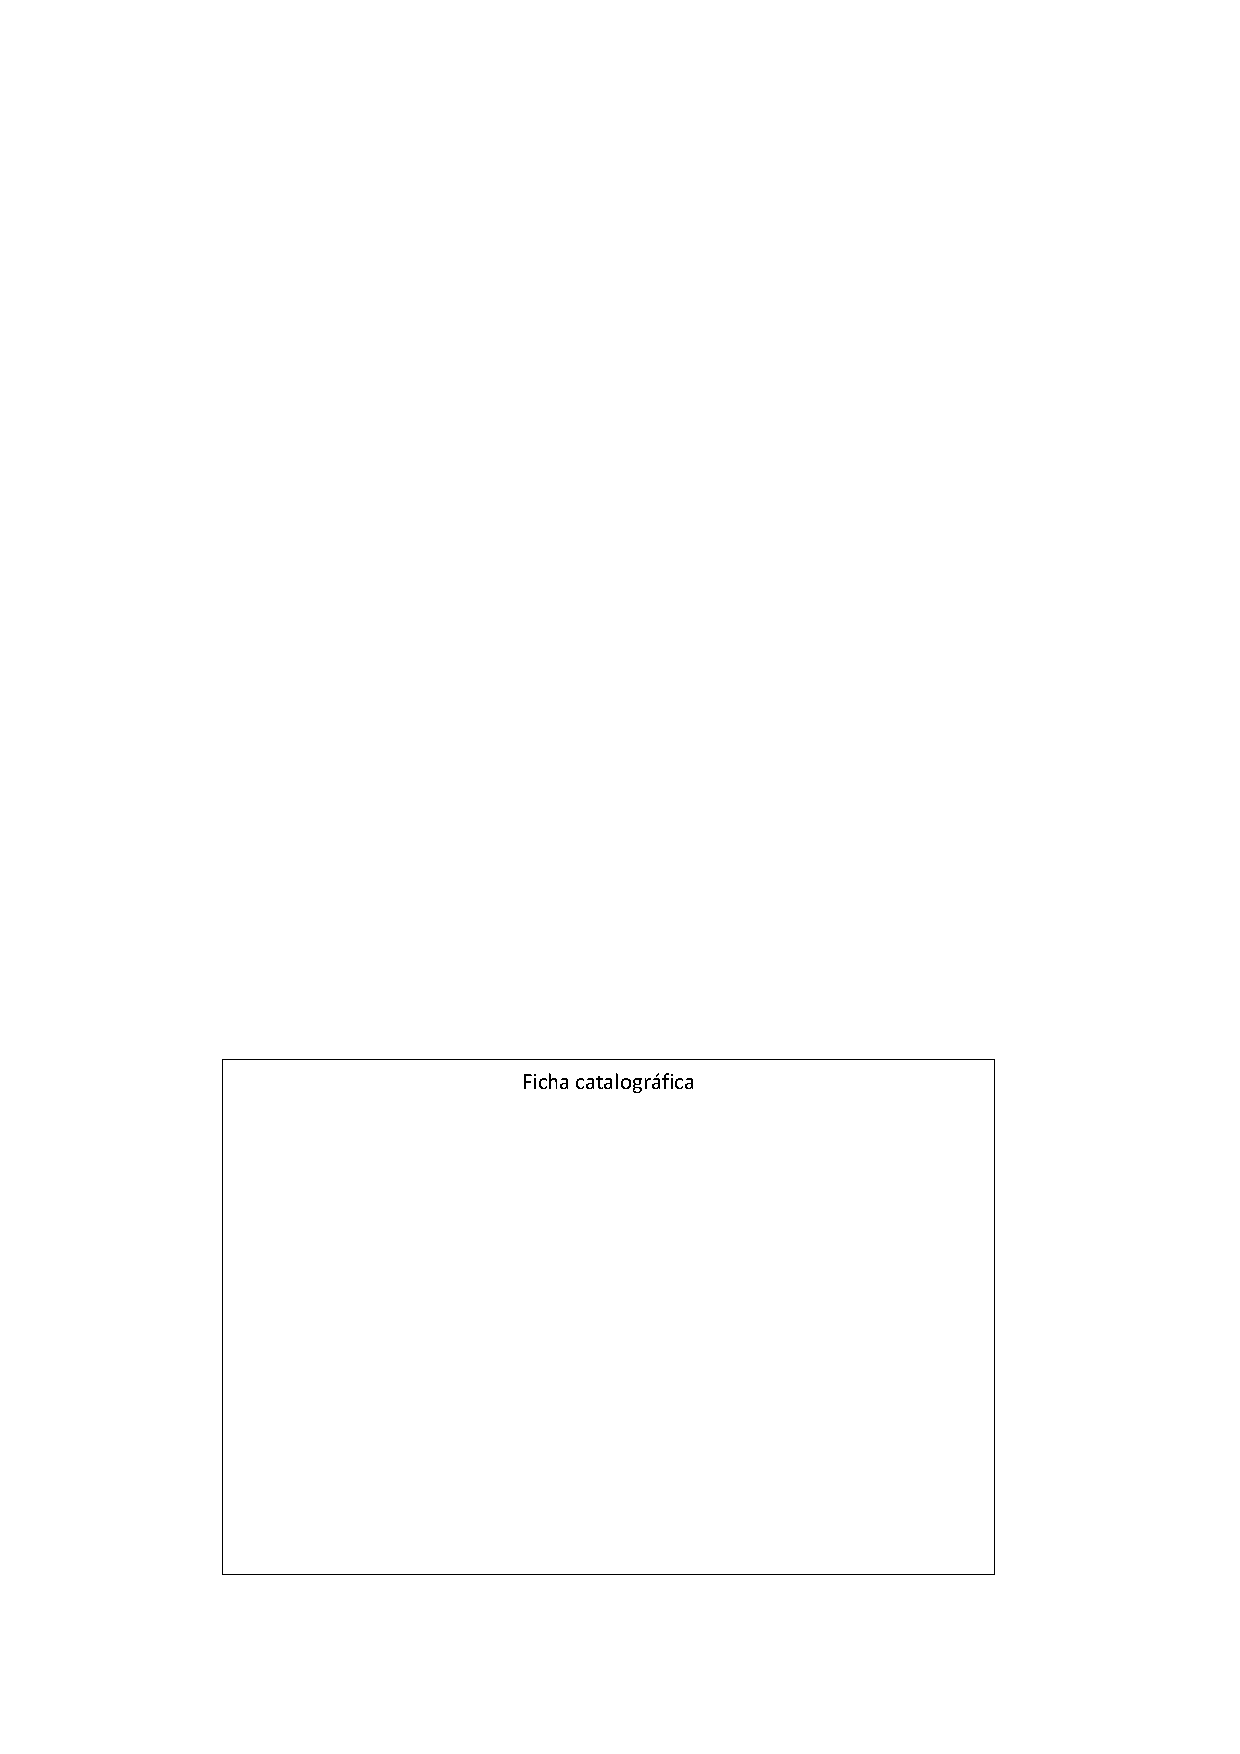
\includepdf{ficha_catalografica.pdf}
\end{fichacatalografica}

\begin{folhadeaprovacao}
	
	\begin{center}
		{\ABNTEXchapterfont\large\imprimirautor}
		
		\vspace*{\fill}\vspace*{\fill}
		\begin{center}
			\ABNTEXchapterfont\bfseries\Large\imprimirtitulo
		\end{center}
		\vspace*{\fill}
		
		\hspace{.45\textwidth}
		\begin{minipage}{.5\textwidth}
			\imprimirpreambulo
		\end{minipage}%
		\vspace*{\fill}
	\end{center}
	
	Trabalho aprovado. \imprimirlocal, 31 de dezembro de 2020:
	
	\assinatura{\textbf{\imprimirorientador} \\ Orientador} 
	\assinatura{\textbf{\imprimircoorientador} \\ Coorientador} 
	\assinatura{\textbf{Professor} \\ Convidado 1}
	\assinatura{\textbf{Professor} \\ Convidado 2}
	
	\begin{center}
		\vspace*{0.5cm}
		{\large\imprimirlocal}
		\par
		{\large\imprimirdata}
		\vspace*{1cm}
	\end{center}
	
\end{folhadeaprovacao}

% Resumo em português
\setlength{\absparsep}{18pt} % Ajusta o espaçamento dos parágrafos do resumo
\begin{resumo}
	A mudança de paradigma na indústria referente às recentes modificações em relação às tecnologias de manufatura é chamada de Indústria 4.0 (I4.0). Nesse novo conceito, redes inteligentes de máquinas e processos para indústria com o respaldo de Tecnologias da Informação e Comunicação (TIC) passam a proporcionar um alto nível de automação e intercâmbio de informações entre equipamentos, produtos e demais atores em um ambiente de manufatura.
	Este trabalho aborda uma proposta de desenvolvimento dos detalhes do Modelo de Arquitetura de Referência para a Indústria 4.0 (RAMI4.0), especificamente por meio da introdução do conceito de Memória Digital do Produto (MDP) ao eixo horizontal ``Ciclo de Vida e Cadeia de Valor'', de forma a se aperfeiçoar a elaboração dessa arquitetura, proporcionando mais robustez ao modelo para uma futura adoção generalizada por parte de empresas por todo o mundo.
	O estudo aborda uma nova estrutura de compartilhamento da MDP do ativo por meio de \textit{Web Services} composta por quatro elos: O Componente I4.0, o Repositório, a MDP e o Cliente. A proposta de estrutura é tratada com base no RAMI4.0 e visa propiciar o surgimento de novos cenários de criação de valor no contexto da I4.0 e incentivar a geração de novos modelos de negócio baseado em dados.
	
	\textbf{Palavras-chave}: Indústria 4.0. RAMI4.0. Memória digital do produto. Arquitetura Orientada a Serviços (SOA). Cadeia de Suprimentos.
\end{resumo}

% Resumo em inglês
\begin{resumo}[Abstract]
	\begin{otherlanguage*}{english}
		This is the english abstract.
		
		\vspace{\onelineskip}
		
		\noindent 
		\textbf{Keywords}: Industry 4.0. RAMI4.0. Digital product memory. Value Chain. Product life cycle. 
	\end{otherlanguage*}
\end{resumo}

% Lista de ilustrações
\pdfbookmark[0]{\listfigurename}{lof}
\listoffigures*
\cleardoublepage

% Lista de tabelas
% ---
\pdfbookmark[0]{\listtablename}{lot}
\listoftables*
\cleardoublepage

% Lista de abreviaturas e siglas
\begin{siglas}
	\item[AAS] \textit{Asset Administration Shell} (Camada Administrativa do Ativo)
	\item[API] \textit{Application Programming Interface} (Interface de Programação de Aplicação)
	\item[BI] \textit{Business Intelligence} (Inteligência Empresarial)
	\item[CS] Cadeia de Suprimentos
	\item[CV] Cadeia de Valor
	\item[CVP] Ciclo de Vida do Produto
	\item[GCVP] Gestão do Ciclo de Vida do Produto
	\item[GI] Gestão da Informação
	\item[I4.0] Indústria 4.0
	\item[IIoT] \textit{Industrial Internet of Things} (Internet das Coisas Industrial)
	\item[IoT] \textit{Internet of Things} (Internet das Coisas)
	\item[MDP] Memória Digital do Produto
	\item[OSI] \textit{Open System Interconnection} (Interconexão aberta de sistemas)
	\item[RAMI4.0] \textit{Reference Architectural Model Industrie 4.0} (Modelo de Arquitetura de Referência para a Indústria 4.0)
	\item[REST] \textit{Representational State Transfer} (Transferência Representacional de Estado)
	\item[RFID] (\textit{Radio-Frequency IDentification}) (Identificação por Radiofrequência)
	\item[SOA] \textit{Service Oriented Architecture} (Arquitetura Orientada a Serviços)
  	\item[TIC] Tecnologia da Informação e Comunicação
  	\item[UUID] \textit{Universal Unique IDentifier} (Identificador Único Universal)
  	\item[WS] \textit{Web Service} (Serviço Web)
  	\item[WSD] \textit{Web Services Description} (Descrição do Serviço Web)
  	\item[WSDL] \textit{Web Services Description Language} (Linguagem de Descrição de Serviços Web)
\end{siglas}

% Sumário
\pdfbookmark[0]{\contentsname}{toc}
\tableofcontents*
\cleardoublepage


% Elementos textuais
\textual
\chapter{Introdução}

	O cenário atual de comércio em um mundo intrinsecamente globalizado requer eficiência em troca de informações, serviços e mercadorias; ou seja, eficiência logística. A logística é a essência do comércio \cite{ballou2006cadeiasuprimentos}, ela contribui para que pessoas não mais sejam obrigadas a viver perto das fontes de produção e possam trocar mercadorias com outras regiões de forma efetiva, contribuindo decisivamente para melhorar o padrão econômico de vida geral. 
	
	A logística é o processo de planejamento, implantação e controle do fluxo eficiente e eficaz de mercadorias, serviços e das informações relativas desde o ponto de origem até o ponto de consumo com o propósito de atender as exigências dos clientes \cite{cscmp2013supplychainglossary}. Essa definição sugere a logística como um processo, o que significa que inclui todas as atividades importantes para a disponibilização de bens e serviços aos consumidores quando e onde estes quiserem adquiri-los \cite{ballou2006cadeiasuprimentos}.
	
	A cadeia de suprimentos (CS), por outro lado, é um conceito mais amplo. A CS é onde a logística é exercida. São as partes necessárias para se dar suporte ao pedido de um cliente, desde o produtor até o consumidor final. A gestão da cadeia de suprimentos tem como alvo a orquestração de todas as partes envolvidas por meio de uma logística integrada de forma a se otimizar ao máximo o processo de fornecimento de um produto, serviço ou informação.
	
	A ideia de uma CS simples envolve fornecedor, produtor e cliente \cite{hugos2018supplychain}, porém conceitos modernos ampliam a noção de CS para uma cadeia de suprimentos estendida, que inclui diversos outros fornecedores de serviços em áreas como logística, finanças, \textit{marketing} e desenvolvimento; que, mediante coordenação e colaboração, criam oportunidades para melhoria dos custos ou serviços ao consumidor. A \autoref{fig:cadeia-de-suprimentos} exemplifica a inter-relação das partes em uma cadeia de suprimentos estendida.
		
	\begin{figure}[htb]
		\centering
		\label{fig:cadeia-de-suprimentos}
		\caption{Exemplo de cadeia de suprimentos estendida.}
		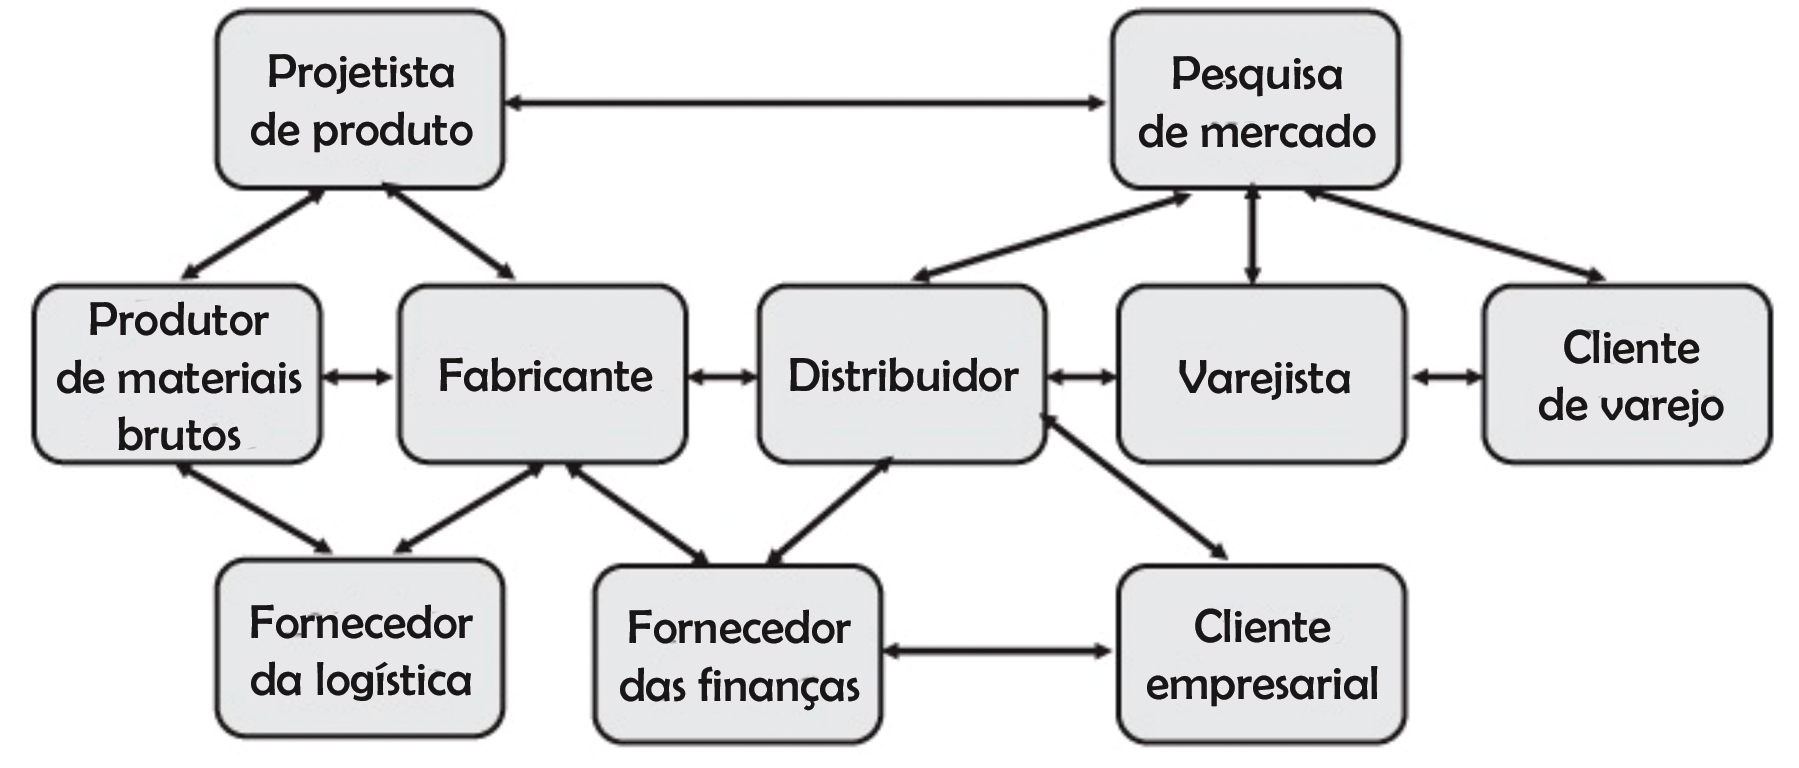
\includegraphics[width=1\textwidth]{cadeia-de-suprimentos.png}
		\fonte{\citeonline{hugos2018supplychain} (adaptado).}
	\end{figure}
	
	Além do eficiente fluxo de materiais e produtos dentro da CS, é imprescindível a manutenção de um canal para troca de informações entre as partes em uma CS, pois sem uma adequada comunicação, gerentes podem acidentalmente tomar decisões supostamente racionais, porém que afetam negativamente outros líderes da cadeia, como o efeito chicote \cite{lee1997bullwhip}, que é a distorção da percepção da procura de um produto que vai se ampliando ao longo da cadeia de suprimentos. Erros de comunicação desse tipo podem acarretar problemas como o aumento do custo de transporte, o elevado tempo de aprovisionamento ao cliente e o desgaste no relacionamento com os fornecedores.
	
	Ao longo da cadeia de suprimentos pode-se observar processos que agregam valor ao produto em desenvolvimento. As etapas de transformação do produto com adição de valor ao longo da CS também podem ser definidas como cadeia de valor.
	
	Uma cadeia de valor (CV) é um conjunto de atividades que empresas de um setor específico desempenham a fim de entregar um produto ou serviço que tenha algum valor perceptível para o mercado \cite{porter1985competitiveadvantage}. A ideia da CV é baseada na agregação de valor ao produto a cada processo de transformação ocorrido, processo esse que envolve a aquisição e consumo de recursos (mão de obra, materiais, equipamentos, instalações, administração, etc). \citeonline{porter1985competitiveadvantage} classifica a CV em duas categorias de atividades que agregam valor ao produto: as atividades primárias e as atividades de apoio (vide \autoref{fig:porter-cadeia-de-valor}).
		
	\begin{figure}[htb]
		\centering
		\caption{Cadeia de valor de Porter.}
		\label{fig:porter-cadeia-de-valor}
		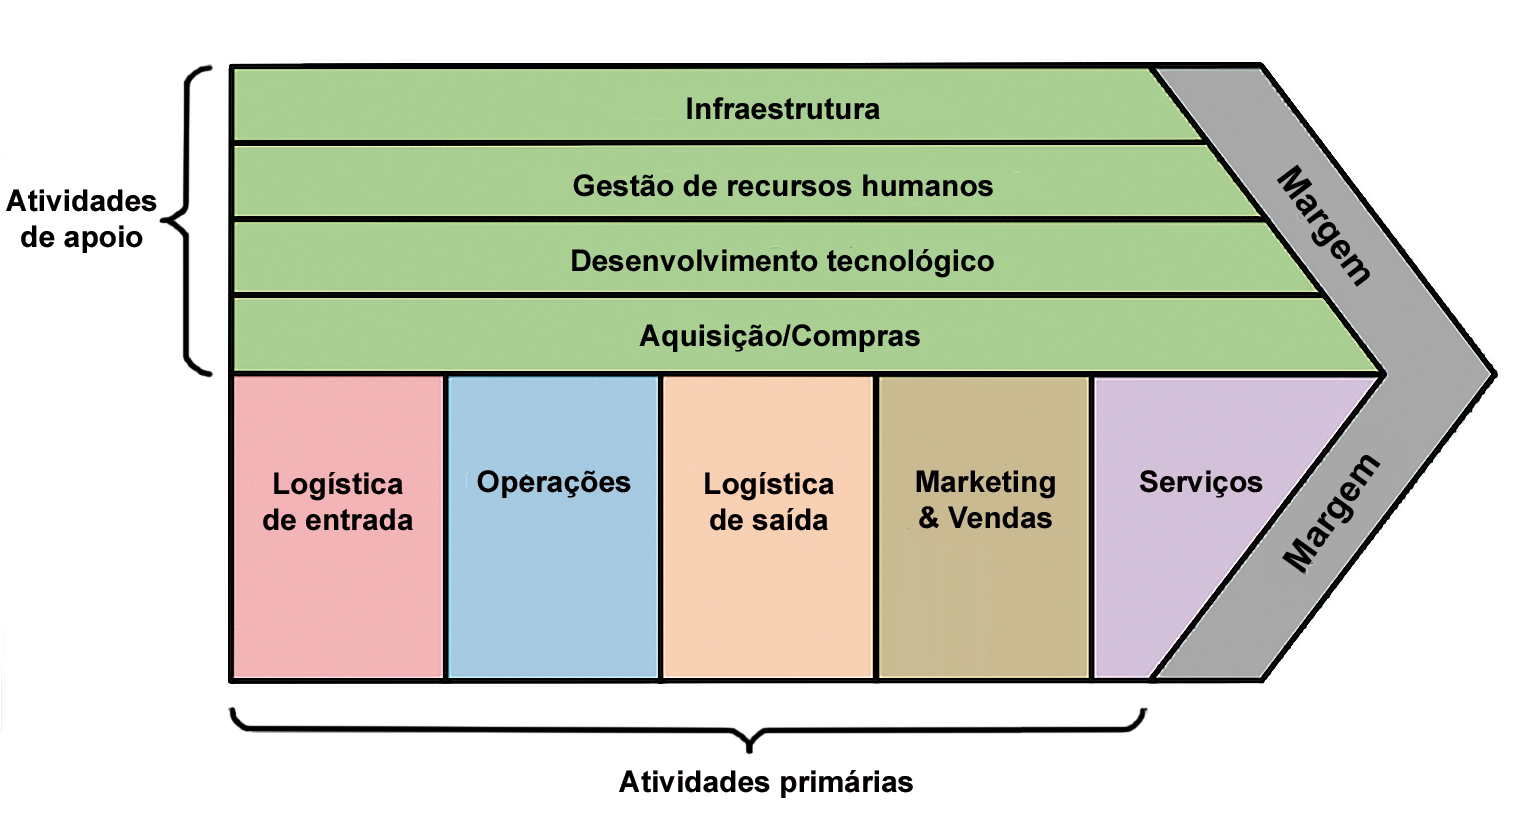
\includegraphics[width=1\textwidth]{porter-cadeia-de-valor.png}
		\fonte{\citeonline{porter1985competitiveadvantage} (adaptado).}
	\end{figure}
	
	As CVs estão focadas em fornecer o máximo valor ao cliente (valor perceptível) com o menor custo e, portanto, é um indicador para a competitividade da empresa. Com o crescente acirramento da competição entre as empresas, essas devem procurar novas formas de agregar mais valor perceptível aos seus produtos, sendo isto em forma de redução de preço, aumento de qualidade, suporte ou qualquer outra nova funcionalidade.
	
	Outra forma de agregação de valor está no princípio de valor compartilhado, que envolve a geração de valor econômico de forma a criar também valor para a sociedade como um todo \cite{porter2011valorcompartilhado} com o enfrentamento de suas necessidades e desafios. Esta necessidade de valor compartilhado parte da percepção generalizada de que empresas prosperam às custas da depreciação da comunidade que as cercam. Soluções que visem o aumento das condições de trabalho, a maior racionalidade e eficiência no tratamento dos recursos naturais necessários para sua atividade e outras formas de balancear o \textit{trade-off} entre eficiência econômica e progresso social são estratégias para se recuperar a legitimidade e a percepção de valor pela sociedade da atividade empresarial.
	
	Atrelado à cadeia de suprimentos e à cadeia de valor existe o conceito de ciclo de vida do produto, que foi um conceito elaborado em meados da década de 1960 com o propósito de criar um modelo que fosse capaz de explicar o sucesso ou fracasso de um produto introduzido ao mercado, sendo capaz também de identificar momentos certos para modificar estratégias de preço, fabricação e quando o produto deve ser descontinuado \cite{cao2012lifecycle}. O modelo inicialmente desenvolvido por \citeonline{levitt1965lifecycle} mostra o padrão de produtos na história passando por quatro estágios bem definidos: desenvolvimento de mercado, crescimento, maturidade e declínio, conforme observado na \autoref{fig:product-life-cycle}.
	
	\begin{figure}[htb]
		\centering
		\caption{Estágios do ciclo de vida do produto.}
		\label{fig:product-life-cycle}
		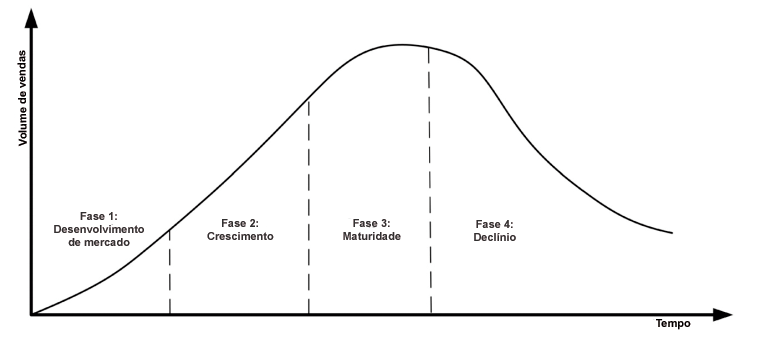
\includegraphics[width=1\textwidth]{product-life-cycle.png}
		\fonte{\citeonline{levitt1965lifecycle} (adaptado).}
	\end{figure}

	Vista a tendência global de redução do ciclo de vida do produto devida a rápida taxa de introdução de novas tecnologias para satisfazer a demanda dos clientes, especialmente no mercado de produtos eletrônicos \cite{trappey2008lifecycle}, novas versões de modelos de ciclo de vida do produto vêm sendo elaboradas considerando outros aspectos de mercado e não somente sob a visão da área de \textit{Marketing}. Por vezes, estudos recentes envolvendo ciclo de vida são denominados ``engenharia do ciclo de vida do produto'' (E-CVP) \cite{cao2012lifecycle} e levam em consideração fatores não abordados nos modelos originais como, por exemplo, a fase de pesquisa e desenvolvimento, a retroalimentação de dados, assim como o descarte e reciclagem do produto. Sempre tendo como objetivo auxiliar na tomada de decisões para o sucesso de um produto no mercado.
	
	A \autoref{fig:life-cycle-extension} mostra um modelo de ciclo de vida do produto com elementos que incluem a fase de desenvolvimento e a renovação do produto. A renovação do produto e a decorrente extensão de sua vida é essencial, pois mantém o produto no mercado na forma de novas versões e, assim, amplia as receitas mediante ações estratégicas para agregação de valor. O modelo do ciclo de vida e os elementos presentes sempre irão variar conforme a natureza do produto e tipo de mercado consumidor onde o mesmo está inserido.
	
	\begin{figure}[htb]
		\centering
		\caption{Modelo de ciclo de vida do produto com renovação do produto.}
		\label{fig:life-cycle-extension}
		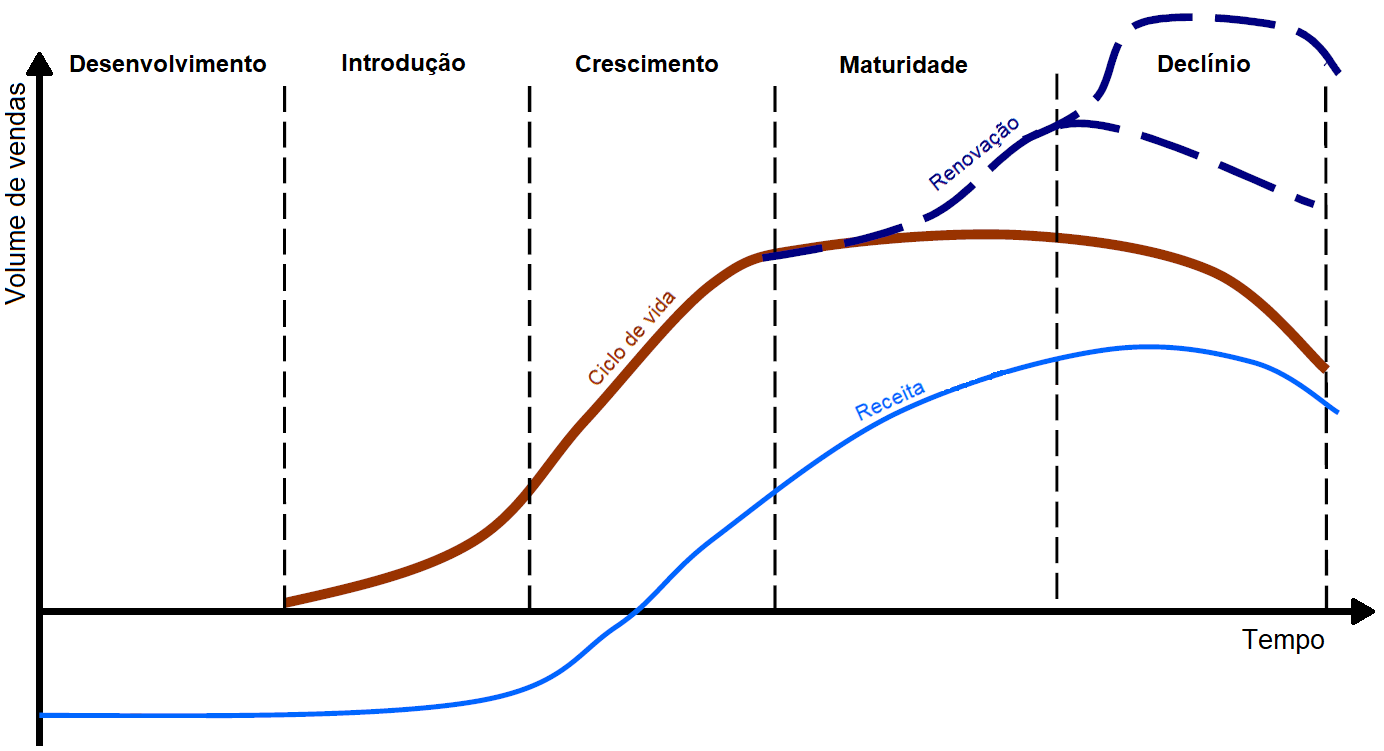
\includegraphics[width=1\textwidth]{life-cycle-extension.png}
		\fonte{\citeonline{liu2010marketingrisk} (adaptado).}
	\end{figure}
	
	Novas propostas de modificações de processos industriais aparecem como formas de se agregar mais valor ao produto/serviço considerando os ciclos de vida do produto cada vez mais curtos. Duas linhas de pesquisas criadas recentemente buscam trazer soluções para os problemas contemporâneos da indústria, como os listados anteriormente, que são os conceitos de Indústria 4.0 (I4.0) e Memória Digital do Produto (MDP).
	
	I4.0 e a MDP são conceitos altamente correlacionados, porém ainda não amplamente abordados em conjunto na literatura, criando assim uma oportunidade de pesquisa a partir de uma lacuna existente.
	
	
\section{Indústria 4.0}

	A crescente integração das Tecnologias da Informação e Comunicação (TIC) às cadeias de valor industriais criou as bases para a próxima revolução industrial chamada Indústria 4.0 \cite{hermann2016design}. Essa mudança de paradigma na indústria se refere às recentes modificações em relação às tecnologias de manufatura, que passam a proporcionar um alto nível de automação e intercâmbio de informações entre equipamentos, produtos e demais atores em um ambiente de manufatura \cite{lasi2014industryfour}. 
	
	O nome Indústria 4.0 (I4.0) se dá ao fato de ser considerada a quarta maior revolução com relação à tecnologia de produção industrial, sendo as ``revoluções industriais'' consideradas evoluções tecnológicas que levaram a grandes mudanças no paradigma de produção, tal histórico de revoluções no campo da indústria é ilustrado na \autoref{fig:i4}.

	\begin{figure}[htb]
		\centering
		\caption{As revoluções industriais.}
		\label{fig:i4}
		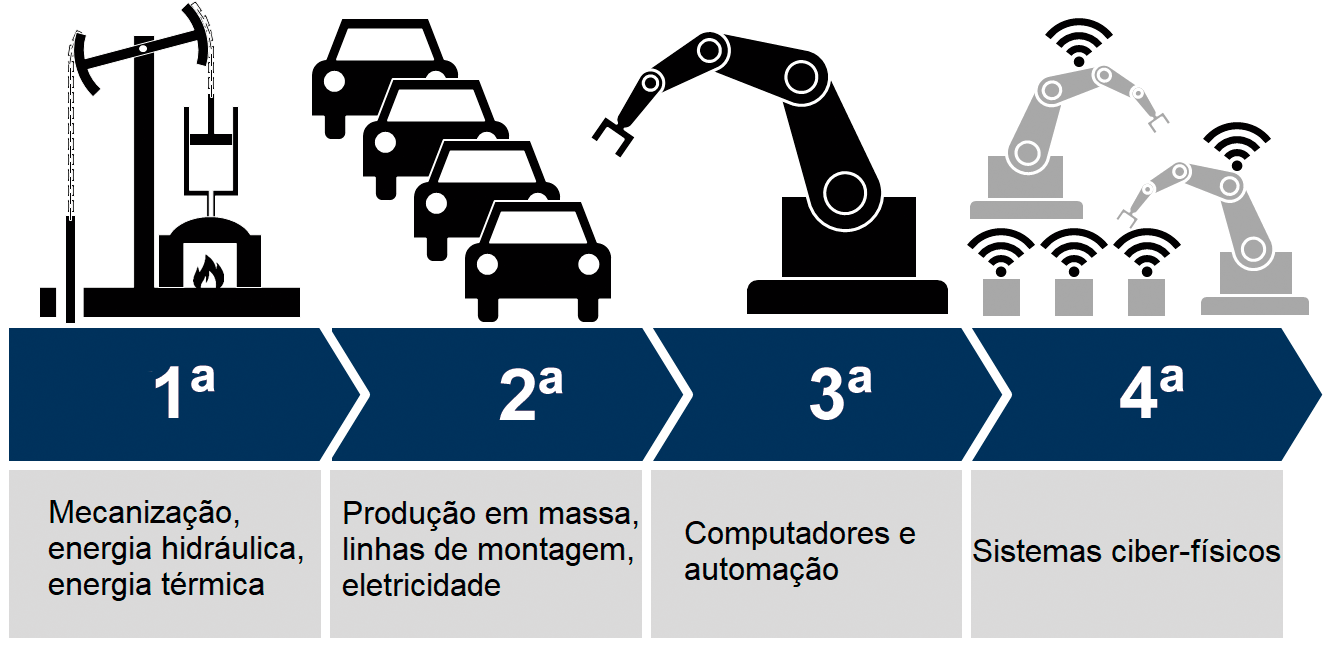
\includegraphics[width=1\textwidth]{i4.png}
		\fonte{\citeonline{lasi2014industryfour} (adaptado).}
	\end{figure}

	Tais modificações na indústria são essenciais devido às novas necessidades da própria indústria e de mudança de padrões de consumo do mercado. Isto acarreta mudanças no cenário operacional destas indústrias. Algumas das causas dessas mudanças operacionais são \cite{lasi2014industryfour}:
	
	\begin{itemize}

		\item Períodos de desenvolvimento curtos: Os períodos de desenvolvimento e inovação de produtos estão sendo reduzidos. A alta capacidade de inovação está se tornando um fator de sucesso para muitas empresas (\textit{Time to market});
		
		\item Individualização sob demanda: Os compradores passam a definir as condições de compra. Essa tendência leva a uma crescente individualização de produtos com características altamente personalizadas e, em casos extremos, a produtos individuais;
		
		\item Flexibilidade: Devido à individualização sob demanda, novas estruturas e organizações na indústria são essenciais para a fabricação de produtos com alto grau de personalização. É necessária uma maior flexibilidade no desenvolvimento do produto, especialmente na produção;
		
		\item Descentralização: Para lidar com condições específicas de cada produto, são necessários procedimentos mais rápidos de tomada de decisão. Para isso, as hierarquias organizacionais precisam ser reduzidas, dando ao produto maior independência sobre seu próprio processo de fabricação;
		
		\item Eficiência de recursos: A maior eficiência sobre o uso dos recursos sempre é algo desejável, porém sua importância se intensifica com as tendências de aumento dos preços dos recursos, bem como a mudança social no contexto de aspectos ecológicos. Isto exige um foco mais intensivo em sustentabilidade, o que decorre em uma maior racionalidade (ou eficiência) na utilização dos recursos.

	\end{itemize}

	Embora o termo I4.0 seja bastante comum na discussão tecnológica atual, muitas empresas, centros de pesquisa e universidades não mantém uma definição comum sobre o assunto. Segundo \citeonline{hermann2016design} e com base em uma revisão de literatura feita pelo mesmo autor, a I4.0 é identificada por quatro princípios de projeto para sua implementação, conforme listados na \autoref{tab:principios-i4}.


	\begin{table}[htb]
		\centering
		\footnotesize
		\caption{Princípios para implantação da I4.0 baseados em \citeonline{hermann2016design}}
		\label{tab:principios-i4}
		\begin{tabular}{p{3cm}p{12cm}}
			\hline
			\textbf{Princípio} & \textbf{Descrição} \\
			
			\hline
			Interoperabilidade &
			Capacidade das coisas (máquinas, dispositivos, sensores, pessoas, etc) de comunicarem entre si dentro de um sistema por meio de padrões definidos. \\
			
			\hline
			Transparência de informação &
			Tornar acessíveis informações úteis para os demais dispositivos conectados à rede. Informações do mundo virtual como documentos eletrônicos, desenhos, modelos de simulação; e informações sobre o mundo real, como posição, dados de sensores de temperatura, vibração, etc. \\
			
			\hline
			Descentralização de decisões &
			Tomada de decisões baseadas nas informações coletados pelo próprio dispositivo da ao dispositivo autonomia para decidir qual será sua próxima função/operação. Desta forma, um planejamento ou controle central de processos produtivos não se faz essencial e o sistema de produção se torna menos hierarquizado. \\
			
			\hline
			Assistência técnica &
			Devido à complexidade da produção, com redes complexas e tomada decisões descentralizadas, os seres humanos precisam ser auxiliados por sistemas de assistência, de forma a dar compreensibilidade ao processo e às tomadas de decisão necessárias. Os sistemas de assistência devem agregar e tornar visualizável as informações de maneira compreensível. \\
			
			\hline
		\end{tabular}
		\fonte{O autor.}
	\end{table}

	Os princípios elencados na \autoref{tab:principios-i4} são diretrizes para o desenvolvimento de arquiteturas para a I4.0. As arquiteturas surgem com a necessidade de se definir padrões para a implantação de um sistema. Por ser um assunto novo, as arquiteturas de sistemas produtivos voltadas para a quarta revolução industrial também se encontram em estágio inicial \cite{pisching2018arquitetura}. Hoje, o mais consolidado modelo de arquitetura para a Indústria 4.0 é o RAMI4.0 (Modelo de Arquitetura de Referência para a Indústria 4.0). Esse modelo de arquitetura foi apresentado na feira industrial de Hanôver na Alemanha em abril de 2015.
	
	O RAMI4.0 requer uma representação tridimensional, conforme a \autoref{fig:rami4}. Nos três eixos do RAMI4.0 são descritos os níveis hierárquicos de uma fábrica ligada em rede através da Internet (Eixo Níveis Hierárquicos), a representação de arquitetura dos componentes I4.0 (Eixo Camadas) e o ciclo de vida de instalações e de produtos (Eixo Ciclo de Vida e Cadeia de Valor).
	
	\begin{figure}[htb]
		\centering
		\caption{Representação do RAMI4.0.}
		\label{fig:rami4}
		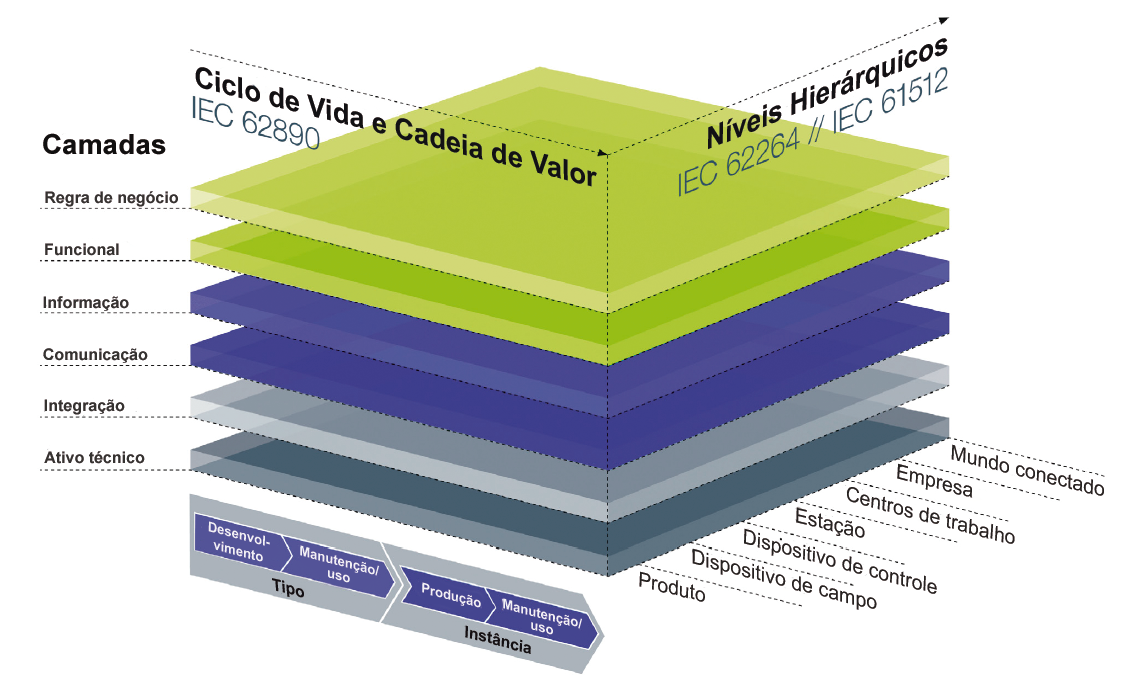
\includegraphics[width=1\textwidth]{rami4.png}
		\fonte{\citeonline{adolphs2015rami} (adaptado).}
	\end{figure}

	O RAMI4.0, como um modelo de referência, é um elemento para padronização do projeto e implantação de aplicações em I4.0. O RAMI4.0 é uma padronização de linguagem e deve ser aceito e usados por todos os participantes para protótipo, desenvolvimento e validação.

\section{Memória Digital do Produto}

	O termo ``Memória Digital do Produto'' (MDP) surgiu pela primeira vez em 2007 por meio de um boletim de notícias de tecnologia de uma empresa alemã fabricante de conectores elétricos e eletrônicos \cite{wahlster2007digitalmemory}. À época, o termo foi tratado com analogia a um diário, que mantinha todas as informações do produto ao longo de seu ciclo de vida.

	Hoje, o conceito na literatura se refere a sistemas que permitem a coleta de dados em todas as fases do ciclo de vida do produto para a distribuição e/ou análise. Os dados de interesse do produto podem ser relativos a qualquer fase do produto ao longo de sua cadeia de valor, o que abrange dados de produção individual, de montagem, de distribuição, de uso por parte do consumidor, etc. A \autoref{fig:MDP-ideia} ilustra o conceito de MDP.
	 
	\begin{figure}[htb]
		\centering
		\caption{Coleta de dados do produto ao longo da cadeia de valores.}
		\label{fig:MDP-ideia}
		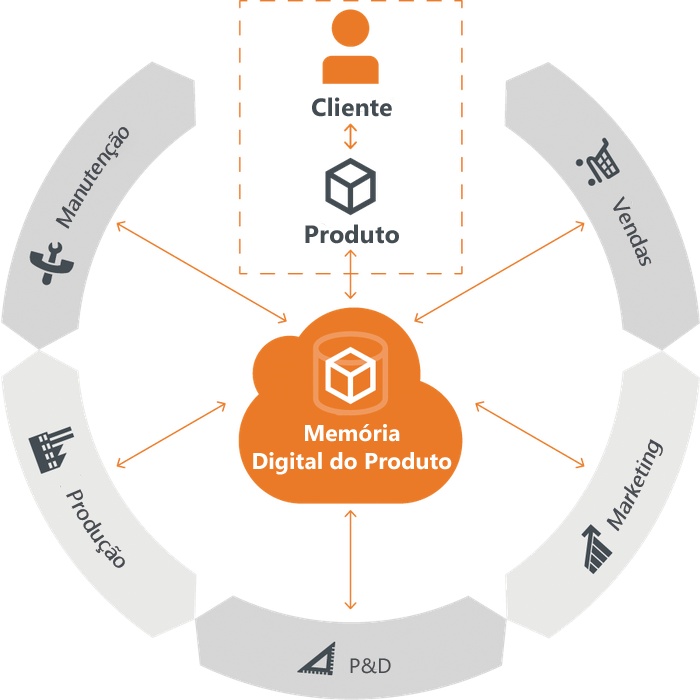
\includegraphics[width=0.6\textwidth]{MDP-ideia.png}
		\fonte{\citeonline{zuhlke2020digitalmemory} (adaptado).}
	\end{figure}

	Sua relevância está no fato da tendência de produtos novos apresentarem ciclos de vida cada vez mais curtos e devido ao fato das cadeias de suprimentos apresentarem redes cada vez mais complexas, com múltiplos fornecedores e clientes. Com isso, a MDP manteria registros digitais do ciclo de vida dos produtos, faria o monitoramento constante do seu estado atual e realizaria o rastreamento de sua posição. Segundo \citeonline{wahlster2007digitalmemory}, o acesso a essas informações pelas partes interessadas seria de vital importância na competitividade de empresa produtoras e de comércio, além de abrir novas proteções em relação à pirataria.
	
	A implementação de uma memória com informações sobre produto ao longo de sua cadeia de valores é importante, pois torna possível acessar e utilizar informações do mundo real providenciada por diferentes fontes ao longo da cadeia de suprimentos para o potencial benefício das partes interessadas naquele produto \cite{brandherm2011productmemory}, como, por exemplo, fabricantes, transportadores, varejistas e consumidores. 
	
\section{Interrelação entre I4.0 e MDP}

 	Ambos os conceitos de I4.0 e MDP são conceitos recentes, surgidos em 2011 \cite{kagermann2011industrie} e 2007 \cite{wahlster2007digitalmemory}, respectivamente . A área multidisciplinar de estudo envolvendo MDP e I4.0 surgira em 2013 com o projeto SemProM \cite{wahlster2013semprom}, porém ainda quando I4.0 era um conceito abrangente e sem diretrizes concretas para sua implementação, que ocorreria em 2013 por meio do documento de recomendações para implementação da iniciativa estratégia Industrie 4.0 \cite{kagermann2013recommendations}; e sem a criação do modelo de arquitetura de referência para Indústria 4.0 (RAMI4.0), que seria divulgada em 2015 por meio do documento entitulado ``RAMI4.0'', divulgado por um periódico alemão \cite{hankel2015rami}.
 	
 	 Alguns outros estudos como \citeonline{lasi2014industryfour} citam MDP como oportunidade de estudo e aplicação dentro da I4.0, outros como \citeonline{weyer2015standardization} e \citeonline{paelke2014augmented} implementam sistemas práticos envolvendo ambos os conceitos, porém sem considerações sobre cadeia de valor.
 	
	Há estudos na área multidisciplinar de I4.0 e MDP, principalmente no meio acadêmico, empresarial e governamental alemão pelo fato de esses conceitos terem surgido na Alemanha. Porém nenhum trabalho até o presente momento relaciona o modelo de arquitetura de referência para a I4.0 (RAMI4.0) com a MDP, o que aponta uma lacuna de conhecimento dentro de I4.0 a ser explorada.
	
	Estudos sobre o RAMI4.0 são importantes no sentido de padronizar a implementação da I4.0 em empresas de diferentes negócios, garantindo assim a interoperabilidade dos serviços. O eixo ``Ciclo de Vida e Cadeia de Valor'' apresenta diretrizes para o correto planejamento da vida de um produto e sugere cenários para criação de valor perceptível ao produto/serviço. Integrar o conceito de MDP ao RAMI4.0, especificamente ao eixo de ``Ciclo de Vida e Cadeia de Valor'', enriquece o nível de discussão sobre essa arquitetura de referência e dá mais robustez ao modelo para uma futura adoção generalizada por parte de empresas por todo o mundo.
	
	A ``Plattform Industrie 4.0'' é uma das principais redes mundiais de discussão sobre I4.0 \cite{kagermann2013recommendations, acatech2014plattform, germany2019plattform}. O Conselho de Pesquisa da Plattform Industrie 4.0 é o comitê consultivo estratégico da Plattform Industrie 4.0 e identifica necessidades de pesquisa e ações em torno da I4.0. O comitê identificou e definiu quatro temas-chave de abordagens no setor tecnológico, econômico, metodológico e social/legal para se implementar com sucesso a I4.0 \cite{hirsch-kreinsen2019keythemes}, conforme mostrado na \autoref{fig:keythemes-i4}. Isso significa que os tópicos elencados são temas com alto potencial para a otimização de rotinas e processos de produção existentes no cenário de I4.0.
	
	\begin{figure}[htb]
		\centering
		\caption{Temas-chave de pesquisa e desenvolvimento em I4.0.}
		\label{fig:keythemes-i4}
		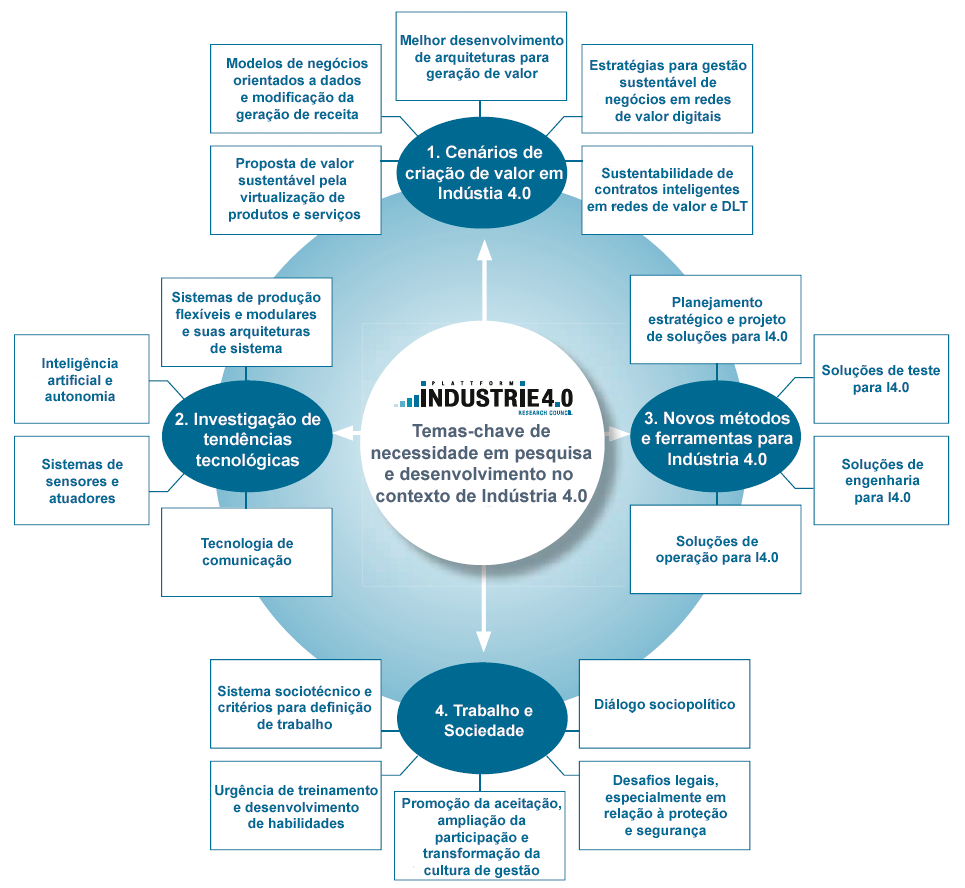
\includegraphics[width=1\textwidth]{keythemes-i4.png}
		\fonte{\citeonline{hirsch-kreinsen2019keythemes} (adaptado).}
	\end{figure}

	Dentre os temas elencados na \autoref{fig:keythemes-i4}, destacam-se os subitens relacionados ao tópico ``Cenários de criação de valor em Indústria 4.0'' por estarem altamente relacionados ao RAMI4.0 e ao conceito de geração de valor por meio da MDP. O desenvolvimento de arquiteturas para geração de valor e a criação de negócios orientados a dados são temas de grande oportunidade dentro do cenário de I4.0, especialmente se considerando os métodos quantitativos de \textit{Business Intelligence} e de análise de dados já estabelecidos.
	

\section{Objetivos da pesquisa}

	O objetivo do trabalho de pesquisa é a investigação da integração do conceito de MDP ao RAMI4.0, especificamente ao eixo de ``Ciclo de Vida e Cadeia de Valor'', de forma a se aperfeiçoar a elaboração dessa arquitetura a fim de proporcionar mais robustez ao modelo para uma futura adoção generalizada por parte de empresas por todo o mundo.
	
	Todo o estudo é feito com a proposta de aperfeiçoar o RAMI4.0 no sentido de propiciar o surgimento de novos cenários de criação de valor no contexto de I4.0 e incentivar geração de novos modelos de negócio baseado em dados.
	
	Este plano de pesquisa envolve o estudo de diversos temas relacionados à Indústria 4.0. Os principais itens estão explicitados a seguir. Diversos novos itens são adicionados ao foco de pesquisa à medida que há aprofundamento nos itens abaixo.
	
	\begin{itemize}
		\item Indústria 4.0;
		\item RAMI4.0;
		\item Cadeia de valor;
		\item Ciclo de vida do produto;
		\item Memória digital do produto;
		\item Internet das coisas.
	\end{itemize}
	
	Tais temas são estudados a fim de se analisar o estado da arte atual em I4.0 e a partir disso propor alterações sobre o RAMI4.0 incluindo o conceito de MDP.
	
\chapter{Metodologia}
\label{cha:metodologia}

	O trabalho é executado a partir de revisão bibliográfica de textos acadêmicos, como dissertações e teses, artigos publicados em revistas acadêmicas, livros teóricos e notas de estudos técnicos. A revisão bibliográfica tem o objetivo de se inteirar do estado da arte das tecnologias envolvidas na Indústria 4.0.
	
	As disciplinas obrigatórias do programa de pós-graduação cursadas durante o período do mestrado foram selecionadas com base na relevância e relacionamento com a natureza da pesquisa em Indústria 4.0 e incluem disciplinas também de outros programas de pós-graduação, como o de Engenharia Elétrica, Engenharia de Transportes e Engenharia de Produção.
	
	A metodologia adotada neste projeto é baseada na proposta por \citeonline{jensen1997petrinet}, onde as etapas de pesquisa são compostas por um ciclo repetitivo de três aspectos, sendo elas: as teorias, as ferramentas e as aplicações; conforme ilustrado na \autoref{fig:metodologia-jensen}.
	
	O próprio conhecimento adquirido nas disciplinas por meio da aprendizagem de novas ``ferramentas'' pode modificar parte das ``aplicações'' e com isso realimentar as ``teorias'' iniciais. Mediante a evolução do projeto ao longo do tempo, novas propostas surgem, e com isso a necessidade do aprendizado de novos conceitos/teorias.

	\begin{figure}[htb]
		\centering
		\caption{Metodologia de pesquisa utilizada.}
		\label{fig:metodologia-jensen}
		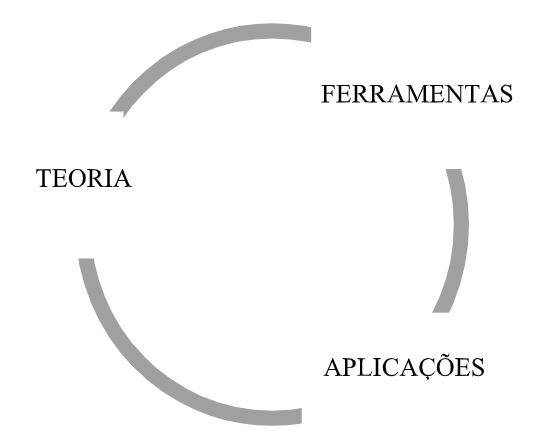
\includegraphics[width=0.7\textwidth]{metodologia-jensen.png}
		\fonte{\citeonline{jensen1997petrinet} (adaptado).}
	\end{figure}

	Aplicando-se a metodologia proposta por \citeonline{jensen1997petrinet} para o caso específico da pesquisa em questão, pode-se listar teorias, ferramentas e aplicações individuais do projeto apresentadas em diferentes fases do projeto de pesquisa.
	
	A \autoref{fig:metodologia-jensen-projeto} mostra os elementos da metodologia de \citeonline{jensen1997petrinet} reformulados em diferentes fases do projeto: (a) na proposta inicial do projeto de pesquisa, (b) no relatório anual após um ano de pesquisa e (c) no texto para a qualificação do programa de mestrado.
	
	\begin{figure}[htb]
		\centering
		\caption{Teorias, ferramentas e aplicações apontadas em diferentes fases do projeto de pesquisa.}
		\label{fig:metodologia-jensen-projeto}
		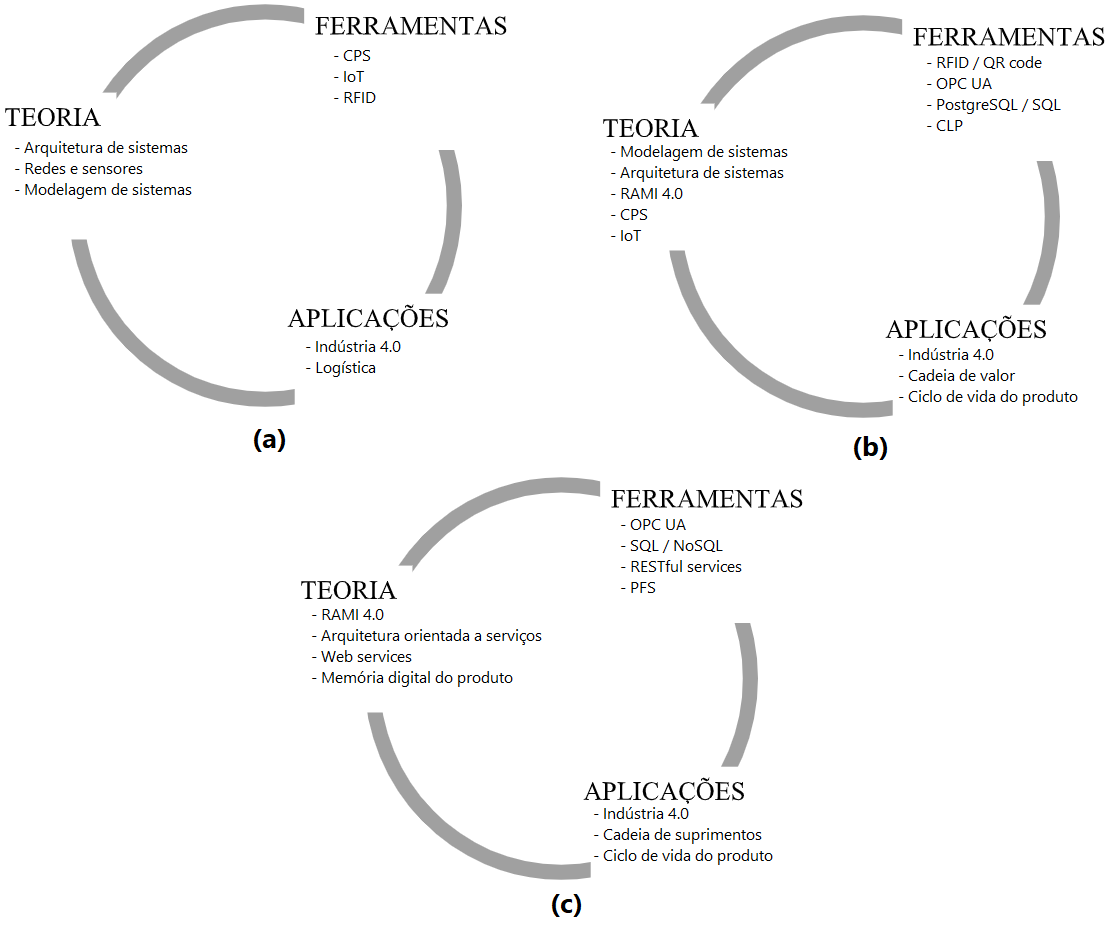
\includegraphics[width=1\textwidth]{metodologia-jensen-projeto.png}
		\fonte{O autor.}
	\end{figure}
	
	 Os ciclos mostrado na \autoref{fig:metodologia-jensen-projeto} se modificam constantemente à medida que o projeto de pesquisa evolui. Portanto, os três aspectos identificados no ciclo devem evoluir simultaneamente, recondicionando-se mutuamente.


\chapter{Fundamentos}
\label{cha:fundamentos}
	
	Nesse capítulo é apresentada a revisão bibliográfica necessária para a fundamentação dos capítulos subsequentes.
	
	Cinco conceitos básicos são apresentados: ``Indústria 4.0'', ``Logística \& Cadeia de Suprimentos'', ``Ciclo de vida do produto'', ``Memória digital do produto'' e ``Arquitetura orientada a serviços''.
	
	A inter-relação entre esses conceitos é a base para o entendimento e criação da arquitetura para o compartilhamento de informações sobre o ativo ao longo da cadeia de suprimentos e para a elaboração de considerações sobre implicações do massivo compartilhamento de informações no ciclo de vida do produto no contexto da Indústria 4.0.

\section{Indústria 4.0}

	Indústria 4.0 (I4.0) é o nome dado às recentes modificações em relação às tecnologias utilizadas em processos industriais e à forma de organização dos sistemas industriais. Tais tecnologias são inseridas com o propósito de se oferecer um alto nível de automação e intercâmbio de informações entre equipamentos e produtos \cite{lasi2014industryfour}.

	O nome I4.0 se dá pelo fato de ser considerada a quarta grande revolução com relação às tecnologias de produção industrial, sendo as ``revoluções industriais'' consideradas evoluções tecnológicas que levaram a grandes mudanças no paradigma de produção. As outras transições dentro da indústria ao longo da história aconteceram: no campo da mecanização da produção (1ª revolução industrial), com a produção em massa e intenso uso de energia elétrica (2ª revolução industrial) e com a expansão da automação e eletrônica (3ª revolução industrial) \cite{lasi2014industryfour}. Tal histórico de revoluções no campo da indústria é ilustrado na \autoref{fig:i4-2}.

	\begin{figure}[htb]
		\centering
		\caption{Evolução da indústria por por meio das revoluções industriais.}
		\label{fig:i4-2}
		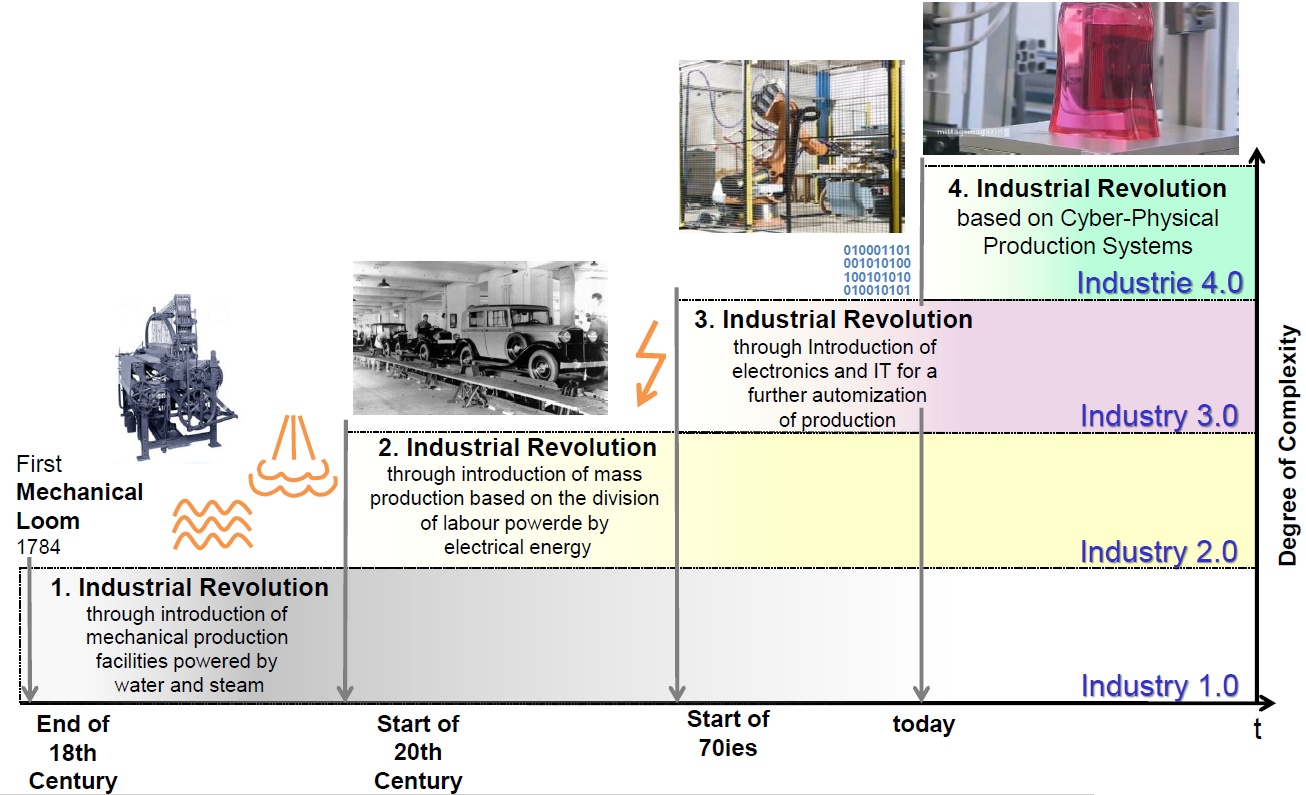
\includegraphics[width=1\textwidth]{i4-2.png}
		\fonte{\citeonline{wahlster2013industrie} (adaptado). }
	\end{figure}

	O termo I4.0 foi trazido a público pela primeira vez em 2011 na feira industrial de Hanôver (\textit{Hannover-Messe}) \cite{kagermann2011industrie}, que é uma feira tecnológica de grande relevância internacional e tem o costume de apresentar grandes inovações relacionadas ao setor industrial.

	Por vezes, a I4.0 é tratada também como a convergência da produção industrial com as novas Tecnologias de Informação e Comunicação (TIC) \cite{hermann2016design}.
	
	Embora o termo I4.0 seja bastante comum na discussão tecnológica atual, muitas empresas, centros de pesquisa e universidades não mantém uma definição comum sobre o assunto. Segundo \citeonline{hermann2016design} e com base em uma revisão de literatura feita pelo mesmo autor, a I4.0 é composta por quatro princípios de projeto para sua implementação, conforme listados na \autoref{tab:principios-i4}.
	
	\begin{table}[htb]
		\centering
		\footnotesize
		\caption{Princípios para implantação da I4.0 baseados em \citeonline{hermann2016design}}
		\label{tab:principios-i4}
		\begin{tabular}{p{3cm}p{12cm}}
			\hline
			\textbf{Princípio} & \textbf{Descrição} \\
			
			\hline
			Interoperabilidade &
			Capacidade das coisas (máquinas, dispositivos, sensores, pessoas, etc) de comunicarem entre si dentro de um sistema por meio de padrões definidos. \\
			
			\hline
			Transparência de informação &
			Tornar acessíveis informações úteis para os demais dispositivos conectados à rede. Informações do mundo virtual como documentos eletrônicos, desenhos, modelos de simulação; e informações sobre o mundo real, como posição, dados de sensores de temperatura, vibração, etc. \\
			
			\hline
			Descentralização de decisões &
			Tomada de decisões baseadas nas informações coletados pelo próprio dispositivo da ao dispositivo autonomia para decidir qual será sua próxima função/operação. Desta forma, um planejamento ou controle central de processos produtivos não se faz essencial e o sistema de produção se torna menos hierarquizado. \\
			
			\hline
			Assistência técnica &
			Devido à complexidade da produção, com redes complexas e tomada decisões descentralizadas, os seres humanos precisam ser auxiliados por sistemas de assistência, de forma a dar compreensibilidade ao processo e às tomadas de decisão necessárias. Os sistemas de assistência devem agregar e tornar visualizável as informações de maneira compreensível. \\
			
			\hline
		\end{tabular}
		\fonte{O autor.}
	\end{table}

	A quarta revolução industrial já está em curso segundo o Fórum Econômico Mundial \cite{schwab2016fourth} em seu encontro anual realizado em Davos no ano de 2016 e as razões para o surgimento desse novo paradigma de produção incluem: a competição acirrada entre empresas, alta complexidade de manufatura dos produtos e seus altos níveis de personalização por parte dos clientes \cite{bordeleau2018bi, vaidya2018industryfour}.

	Uma das bases para esse novo paradigma de produção é a interligação de objetos no ambiente de produção por meio de identificadores individuais usando conceitos de Internet das Coisas (\textit{Internet of Things} - IoT) e de Internet das Coisas Industrial (\textit{Industrial Internet of Things} - IIoT). Tais ``coisas'' se referem a equipamentos, produtos, máquinas, peças, pessoas e quaisquer outros elementos envolvidos no ambiente industrial, por vezes também são denominados ``ativos''.
	
	Esses ativos são inseridos no meio digital, onde podem trocar informações entre si e executarem funções sobre seu respectivo correspondente real de forma mais autônoma e com menor intervenção humana por meio do uso extensivo de recursos avançados de tecnologias da informação e comunicação \cite{adolph2018roadmap}. Devido a essa maior relação entre elementos do sistema de fabricação, extingui-se a relação essencialmente hierarquizada da indústria tradicional e os ativos passam a deter a capacidade de se comunicarem diretamente com outros elementos de diferentes níveis, conforme ilustrado na \autoref{fig:i3-to-i4}.
	
	\begin{figure}[htb]
		\centering
		\caption{Transição do (a) modelo hierárquico tradicional para o (b) modelo flexível de comunicação entre dispositivos na Indústria 4.0.}
		\label{fig:i3-to-i4}
		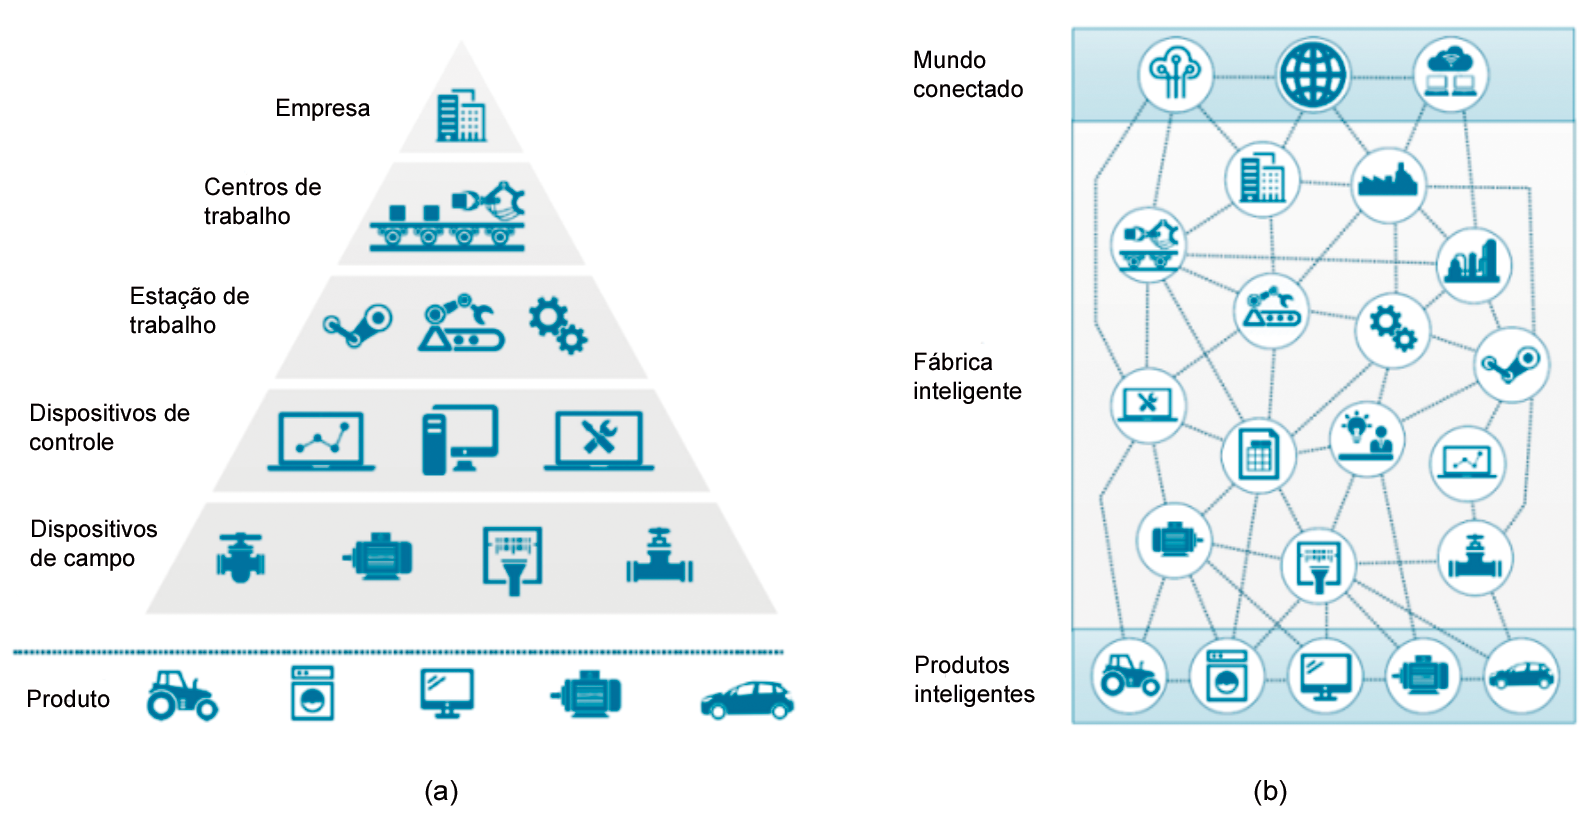
\includegraphics[width=1\textwidth]{i3-to-i4.png}
		\fonte{\citeonline{schmittner2017mtom} (adaptado).}
	\end{figure}

	Essa automatização e a troca de informações entre os ativos tem grande potencial de dar mais eficiência aos processos industriais, pois desta forma o sistema pode tomar decisões ótimas com base nas informações que lhe foram fornecidas por meio de sensores e identificadores. A visão para o futuro da produção baseado na I4.0 envolve sistemas de manufatura modulares e eficientes em cenários nos quais os produtos controlam seus próprios processos de fabricação \cite{lasi2014industryfour}.
	
	Há uma tendência global de redução do ciclo de vida do produto devido à rápida introdução de novas tecnologias para satisfazer a demanda dos clientes, especialmente em produtos eletrônicos \cite{trappey2008lifecycle}. A I4.0 beneficia a chegada de produtos com curto ciclo de vida uma vez que o produto controla seu próprio processo de fabricação, facilitando, assim, ajustes e personalizações por parte do cliente, enquanto preserva os custos, a qualidade e o tempo de aprovisionamento (\textit{lead time}) da produção em massa.
	
	Indústria 4.0 é um conceito. Isto significa que são princípios a serem seguidos e implementados, porém o caminho para a implementação, assim como as tecnologias a serem adotadas podem ser diversos. As peculiaridades de cada indústria e de cada mercado estabelecem diferentes regras de negócios e, portanto, cada setor da indústria pode necessitar de diferentes formas e tecnologias para se implementar a I4.0 e se tornar uma fábrica inteligente. Alguns avanços tecnológicos, entretanto, são muito importantes ou essenciais para a implementação da I4.0 em qualquer sistema de manufatura, alguns deles são mostrados na \autoref{fig:tecnologias-i4}.
	
	\begin{figure}[htb]
		\centering
		\caption{Avanços tecnológicos que moldam a I4.0.}
		\label{fig:tecnologias-i4}
		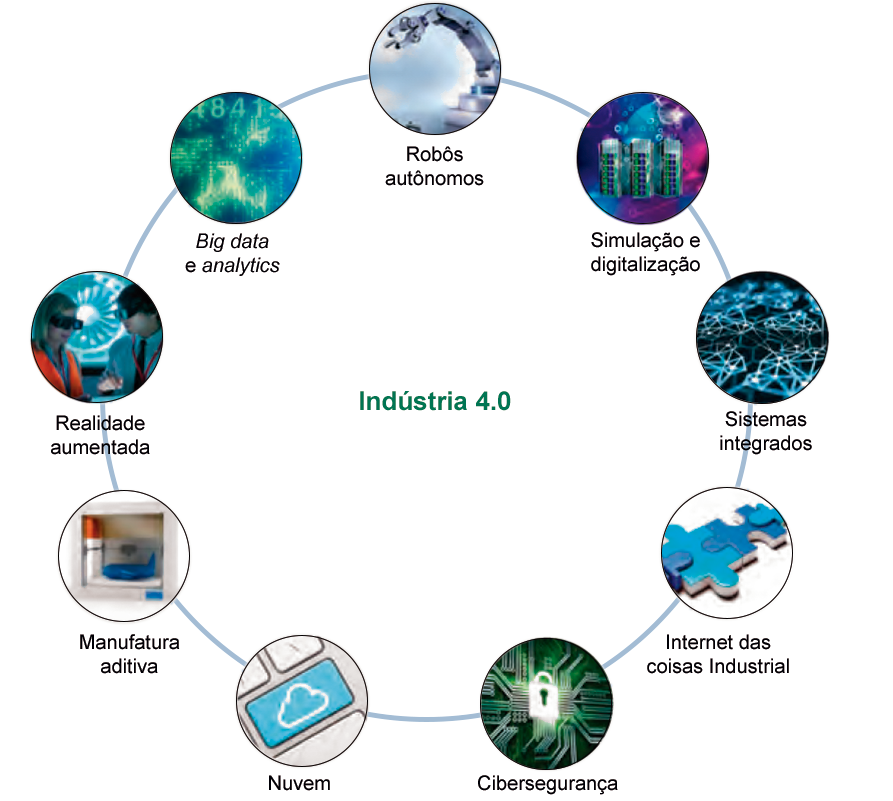
\includegraphics[width=0.9\textwidth]{tecnologias-i4.png}
		\fonte{\citeonline{russmann2015industryfour} (adaptado).}
	\end{figure}

	Após a primeira aparição do termo I4.0 na feira industrial de Hanôver em 2011, o termo ganhou significativa popularidade, principalmente no meio acadêmico e empresarial alemão. O termo foi então incentivado pelo governo alemão \cite{lasi2014industryfour, kagermann2013recommendations}, que apoiou a ideia e anunciou a Indústria 4.0 como parte integral de sua iniciativa estratégica para a indústria alemã, visando liderança em inovação tecnológica \cite{drath2014industrie} como uma abordagem para fortalecer a competitividade da indústria manufatureira alemã.	

	Por meio da iniciativa \textit{Plattform Industrie 4.0}, criada em 2013 pelo Ministério Federal da Educação e Pesquisa (\textit{Bundesministerium für Bildung und Forschung}) \cite{germany2019plattform} e com o grupo de trabalho ``Industrie 4.0 Working Group'' em comunicação com diversas associações de engenharia e indústrias alemãs, foram criados documentos oficiais como os de \citeonline{kagermann2013recommendations}, \citeonline{adolph2018roadmap} e \citeonline{bitkom2016implementation}, publicados em inglês e contendo normas e diretrizes para a implementação da I4.0. Esta iniciativa, atrelada ao entusiasmo acadêmico em torno do projeto I4.0, disseminou o conceito fora da área de língua alemã e popularizou o termo I4.0 no mundo todo como epônimo de um futuro projeto no contexto de indústrias de alta tecnologia.

	O impacto econômico dessa revolução industrial será enorme, pois a I4.0 promete uma eficiência operacional substancialmente maior, bem como o surgimento de modelos de negócios, serviços e produtos de totalmente novos \cite{hermann2016design}.
	
	Em revoluções industriais passadas, os países pioneiros a se adaptarem às drásticas mudanças de produção foram os que mais se beneficiaram e se consolidaram como potências econômicas. Na quarta revolução industrial não será diferente. Embora a mudança completa para a I4.0 possa levar 20 anos para ser concretizada \cite{russmann2015industryfour}, nos próximos anos serão estabelecidos avanços importantes que definirão os pioneiros e detentores de tecnologias dessa nova revolução. Portanto, é de interesse de cada país liderar a concorrência global a fim de se consolidar como mercado líder e fornecedor de soluções para a Indústria 4.0.

	\subsection{Modelo de Arquitetura de Referência para a Indústria 4.0}
	
	O Modelo de Arquitetura de Referência para a Indústria 4.0, abreviado RAMI4.0, consiste em um sistema de coordenadas tridimensional que descreve todos os aspectos cruciais da Indústria 4.0. Dessa maneira, inter-relações complexas podem ser divididas em grupos menores e mais simples.
	
	A \autoref{fig:rami4} mostra a representação do RAMI4.0 e especifica os itens contidos em cada eixo. A \autoref{tab:rami-eixos} fornece uma breve descrição de cada eixo do RAMI4.0.
	
	\begin{table}[htb]
		\centering
		\footnotesize
		\caption{Eixos do RAMI4.0}
		\label{tab:rami-eixos}
		\begin{tabular}{p{3cm}p{12cm}}
			\hline
			\textbf{Eixo} &\textbf{Descrição} \\
			
			\hline
			Camadas
			& As seis camadas no eixo vertical descrevem a decomposição de um ativo em suas funcionalidades, isto é, o mapeamento virtual de um ativo. A representação em camadas se origina da tecnologia da informação e comunicação (TIC), onde as funcionalidades de sistemas complexos são comumente divididas em camadas. \\
			
			
			\hline
			Ciclo de vida e  Cadeia de valor
			& O eixo horizontal esquerdo representa o ciclo de vida das instalações e produtos, com base na IEC 62890 para gerenciamento do ciclo de vida. Além disso, é feita uma distinção entre ``tipos'' e ``instâncias''. Um ``tipo''~ é criado na fase de desenvolvimento e, uma vez concluída esta fase, esse tipo é liberado para a produção, servindo como modelo para uma ``instância'', que é quando produto real está sendo fabricado e possui um número de série. \\
			
			\hline
			Níveis hierárquicos
			& No eixo horizontal direito estão indicados os níveis hierárquicos da IEC 62264, a série de padrões internacionais para sistemas de TI e controle corporativos. Os níveis hierárquicos representam as diferentes funcionalidades das fábricas. Para representar o ambiente I4.0, as funcionalidades foram expandidas, incluindo adicionalmente o ``Produto'' e o ``Mundo conectado''. \\
			\hline
			
		\end{tabular}
		\fonte{O autor.}
	\end{table}

	A \autoref{fig:eixo-camadas} mostra o detalhamento de cada elemento do eixo Camadas do RAMI4.0 e sua associação ao modelo completo.
	
	\begin{figure}[htb]
		\centering
		\caption{(A) Representação completa do RAMI4.0 e (b) Detalhamento de cada elemento do Eixo Camadas.}
		\label{fig:eixo-camadas}
		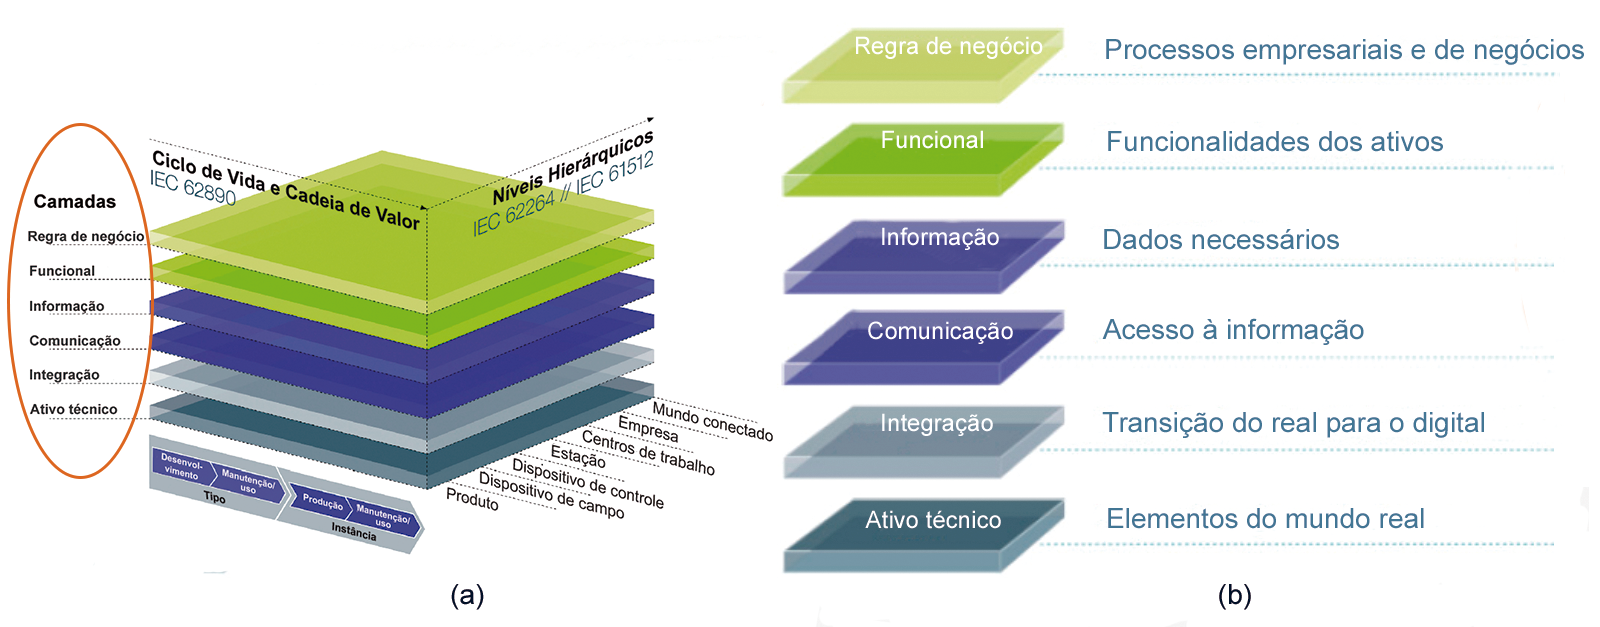
\includegraphics[width=1\textwidth]{eixo-camadas.png}
		\fonte{\citeonline{gayko2018ramistandardization} (adaptado).}
	\end{figure}

	São 6 as camadas do RAMI4.0. O propósito de cada camada, começando da mais inferior (Ativo) para a mais elevada (Regra de Negócio), é descrito a seguir \cite{bitkom2016implementation}:
	
	\begin{enumerate}
		\item \textbf{Ativo}: Representa um elemento da realidade não necessariamente físico, como, por exemplo, uma máquina, um \textit{software}, uma documentação, uma ideia, etc. O trabalhador e seu conhecimento sendo aplicado representa também um ativo. Os ativos são integrados ao meio digital através da camada de Integração.
		
		\item \textbf{Integração}: Camada responsável pela extração e fornecimento de informações sobre os ativos para as camadas superiores. Representa a digitalização dos ativos. Cada evento no mundo real é refletido também em um evento no mundo virtual. Se a realidade mudar, esse evento então é relatado à camada de integração e os dados são atualizados no mundo virtual.
		
		\item \textbf{Comunicação}: Padronização da comunicação por meio da adoção de um formato de troca de dados uniforme entre os dispositivos. Esta camada é a responsável pela interoperabilidade entre os ativos na I4.0. A camada de Comunicação fornece dados sobre o ativo à camada de informação.
		
		\item \textbf{Informação}: Controle dos dados do ativo. Esta camada agrega todos os dados sobre um determinado ativo e é responsável pelo gerenciamento desses dados. Na camada de informação são garantidos que os dados sejam tratados, pré-processados, armazenados e disponibilizados para os demais ativos na rede.
		
		\item \textbf{Funcional}: Contém a descrição formal de todas as funcionalidades do sistema. É também a camada responsável pela integração horizontal de ativos, ou seja, é a porta de interação entre diferentes Componentes I4.0. Esta camada é a interface para o fornecimento de informações por meio de microsserviços para outros ativos tanto dentro (integração vertical) como fora (integração horizontal) da empresa.
			
		\item \textbf{Regra de negócio}: Contêm as regras de negócio que o sistema deve seguir como, por exemplo, as condições legais e regulatórias. Esta camada também é responsável por mapear os modelos de negócios do sistema e orquestrar os serviços da camada funcional.
	\end{enumerate}

	Já os elementos do eixo ``Ciclo de Vida e Cadeia de Valor'' do RAMI4.0 são detalhados na \autoref{fig:eixo-ciclodevida}, juntamente com seu destaque dentro do modelo completo.
	
	\begin{figure}[htb]
		\centering
		\caption{(A) Representação completa do RAMI4.0 e (b) detalhamento do eixo Ciclo de Vida e Cadeia de Valor.}
		\label{fig:eixo-ciclodevida}
		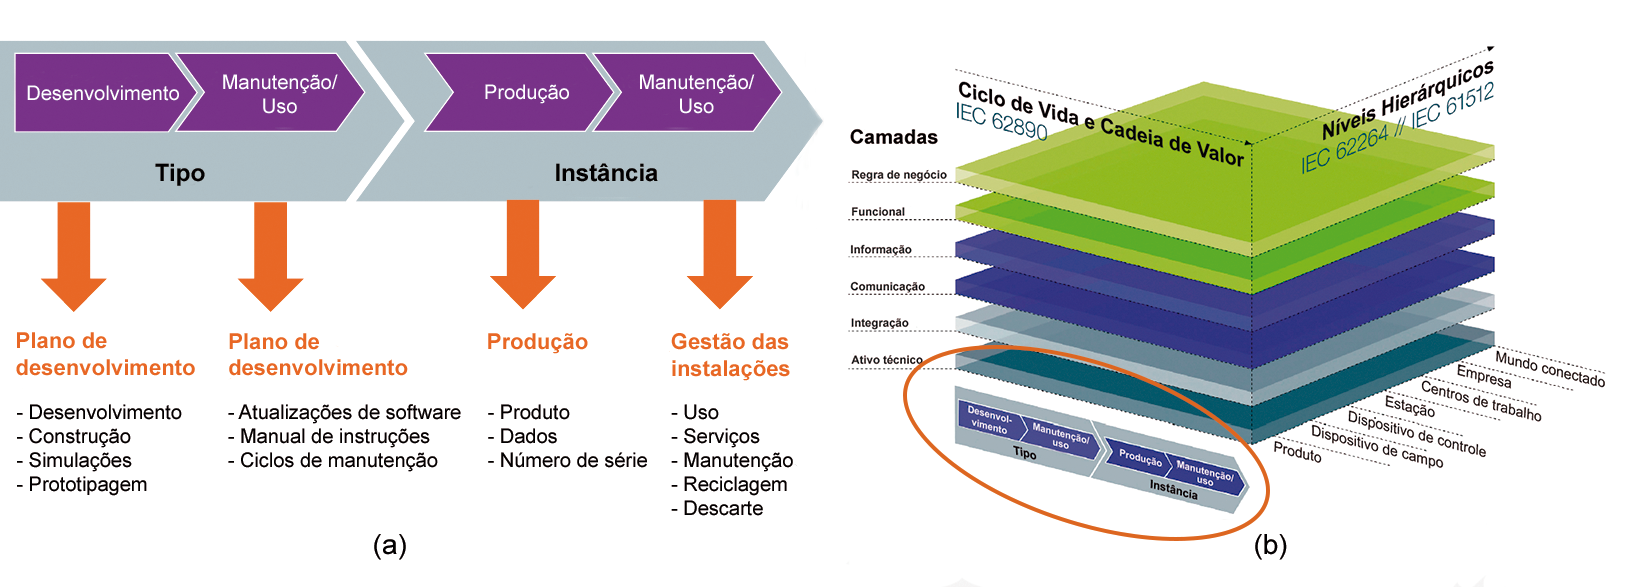
\includegraphics[width=1\textwidth]{eixo-ciclodevida.png}
		\fonte{\citeonline{gayko2018ramistandardization} (adaptado).}
	\end{figure}

	A I4.0 oferece um grande potencial de aprimoramento dos processos ao longo do ciclo de vida do produto. Este eixo fornece uma representação do estado do ativo ao longo de toda sua cadeia de suprimentos e sua cadeia de valor. 
	
	É feita a distinção fundamental entre ``tipo'' e ``instância'', cada um correspondendo a uma fase em que o produto se encontra \cite{adolphs2015rami}.
	
	Um tipo é sempre criado com uma ideia inicial, ou seja, quando um produto surge na fase de desenvolvimento. Isso abrange o comissionamento, desenvolvimento e testes até a produção inicial de amostras e protótipos \cite{adolph2018roadmap}. 
	
	Com a conclusão de todas as etapas de testes e validação, o tipo é liberado para produção em série. A partir de então, novos produtos podem ser instanciados com base neste tipo validado. 
	
	Com a fabricação do produto, instâncias são geradas. Cada produto fabricado representa uma instância de um determinado tipo e recebe um número de série exclusivo.
	
	As melhorias sobre um produto feitas pelo fabricante refletem em um novo tipo, que por sua vez pode ser usado para fabricar novas instâncias, acompanhando, assim, o ciclo de vida do produto.

	O último eixo descrito, ``Níveis Hierárquicos'', do RAMI4.0 é apresentado na \autoref{fig:eixo-niveishierarquicos}.
	
	\begin{figure}[htb]
		\centering
		\caption{(a) Representação completa do RAMI4.0 e (b) detalhamento do eixo Níveis Hierárquicos do RAMI4.0.}
		\label{fig:eixo-niveishierarquicos}
		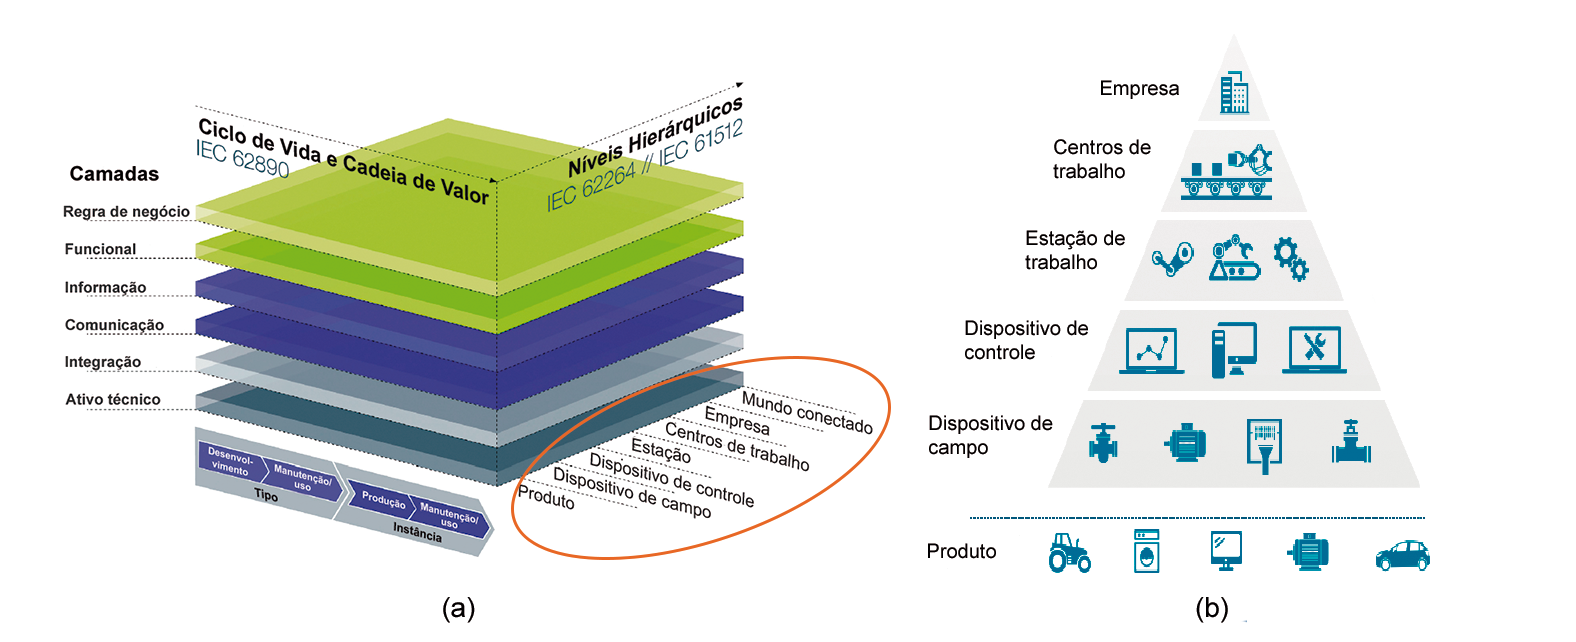
\includegraphics[width=1\textwidth]{eixo-niveishierarquicos.png}
		\fonte{\citeonline{gayko2018ramistandardization} (adaptado).}
	\end{figure}

	Este eixo representa as diferentes funcionalidades das fábricas e descreve a integração dos sistemas empresariais de controle \cite{pisching2018arquitetura}.
	
	Este eixo é baseado em uma reformulação da IEC 62264, que é a série de padrões internacionais para sistemas de TI e controle corporativos, e faz uma alusão à pirâmide da automação industrial da ISA-95.
	
	Os níveis hierárquicos representam as diferentes funcionalidades das fábricas. Para representar o ambiente I4.0, as funcionalidades foram expandidas além da IEC 62264, que já possui os níveis ``Dispositivo de campo'', ``Dispositivo de controle'', ``Estação de trabalho'', ``Centros de trabalho'' e ``Empresa''.
	
	Para a representação do ambiente I4.0, foi adicionado o nível ``Produto'' na posição mais inferior para descrever funcionalidades relacionadas ao produto da manufatura e o nível ``Mundo conectado'' na posição mais superior para descrever o grupo de fábricas e a colaboração entre empresas, fornecedores de componentes, clientes, etc. 
	
	Dentro dos três eixos, todos os aspectos cruciais da I4.0 podem ser mapeados, permitindo que os ativos sejam classificados devidamente de acordo com o modelo. Os conceitos altamente flexíveis da I4.0 podem, assim, ser descritos e implementados usando o RAMI4.0. O modelo de arquitetura de referência permite a migração passo a passo do presente estado da indústria para o mundo da Indústria 4.0.
	
	\subsection{Asset Administration Shell}
	
	Um ativo é qualquer coisa que precise ser conectada para agregar valor a um processo industrial \cite{bader2019aas}, ou seja, todos os itens que têm valor em um caso de uso específico. Na I4.0, isso pode ser um produto físico, uma peça de equipamento, um \textit{Software} ou documentos como plantas, contratos, pedidos, etc.
	
	No paradigma da I4.0, cada ativo é encapsulado por uma camada (ou casca) de administração, esta casca de administração do ativo técnico é denominada \textit{``Asset Administration Shell''} (AAS). O AAS é a representação da parte virtual/digital de um ativo no mundo I4.0 \cite{ye2019aas}.
	
	Fazendo uma associação ao RAMI4.0, o AAS engloba as camadas digitais, sendo elas: Regra de Negócio, Funcional, Informação e Comunicação; parte da camada Integração também é contemplada pelo AAS, já que essa é a conexão entre o ativo e o meio virtual. Tal associação é representada pela \autoref{fig:aas-rami}.

	\begin{figure}[htb]
		\centering
		\caption{Representação do AAS como a parte virtual do Componente I4.0.}
		\label{fig:aas-rami}
		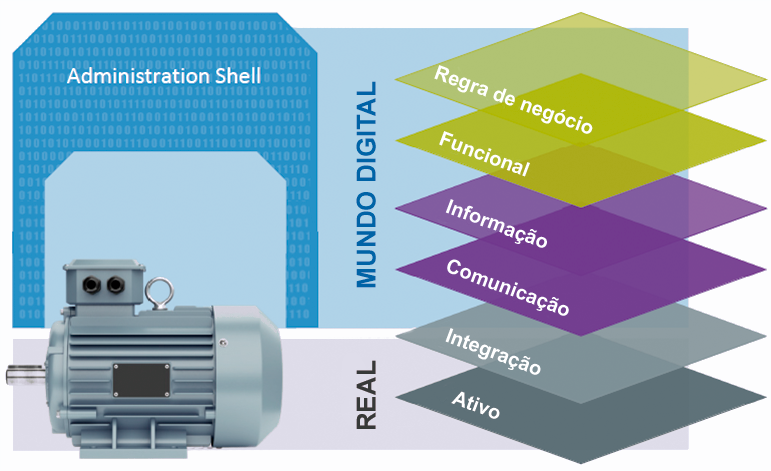
\includegraphics[width=0.8\textwidth]{aas-rami.png}
		\fonte{\citeonline{gayko2018ramistandardization} (adaptado).}
	\end{figure}
		
	O AAS consiste em vários submodelos nos quais são descritos todas as informações e funcionalidades de um determinado ativo, incluindo suas características, propriedades, condição, parâmetros, dados de medições e capacidades \cite{bader2019aas}. A \autoref{fig:aas-submodelos} exemplifica um AAS como sendo uma ``casca'' que engloba o ativo, essa casca contém informações relevantes do ativo em forma de ``submodelos''.
	
	\begin{figure}[htb]
		\centering
		\caption{Exemplificação de um AAS para um servomotor, incluindo os submodelos de identificação, dados técnicos, dados operacionais e documentação.}
		\label{fig:aas-submodelos}
		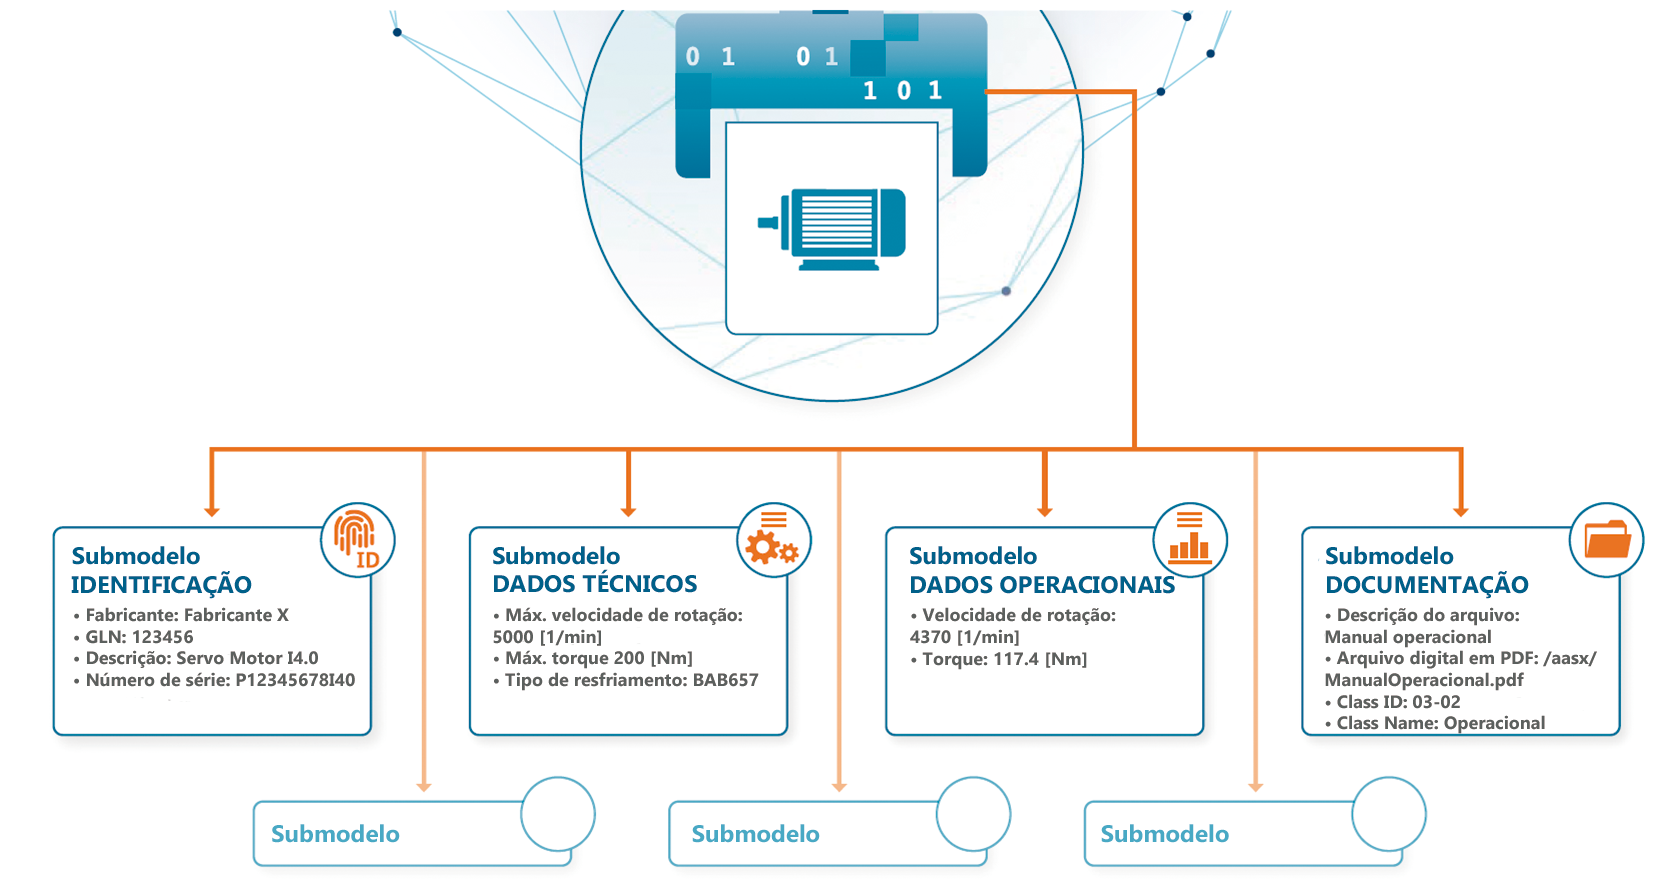
\includegraphics[width=1\textwidth]{aas-submodelos.png}
		\fonte{\citeonline{bader2019aas} (adaptado).}
	\end{figure}

	Os submodelos são unidades básicas de organização dentro de um AAS que agregam informações semelhantes. Eles são divididos em dois tipos \cite{plattform2019detailsaas}: submodelos básicos e submodelos livres \cite{bader2019aas}.
	
	Os submodelos básicos são unidades de organização que se aplicam a muitos ou todos os ativos dentro do mundo I4.0. Já os submodelos livre são acertados entre os parceiros na cadeia de suprimentos e possuem um uso específico para um determinado produto.
	
	O AAS é um elo entre os ativos reais e seus correspondentes digitais no mundo conectado. A \autoref{fig:aas-conexao} ilustra a comunicação entre diferentes AASs em um ambiente de manufatura I4.0 sob uma ontologia comum.
	
	\begin{figure}[htb]
		\centering
		\caption{Comunicação entre AASs de componentes I4.0.}
		\label{fig:aas-conexao}
		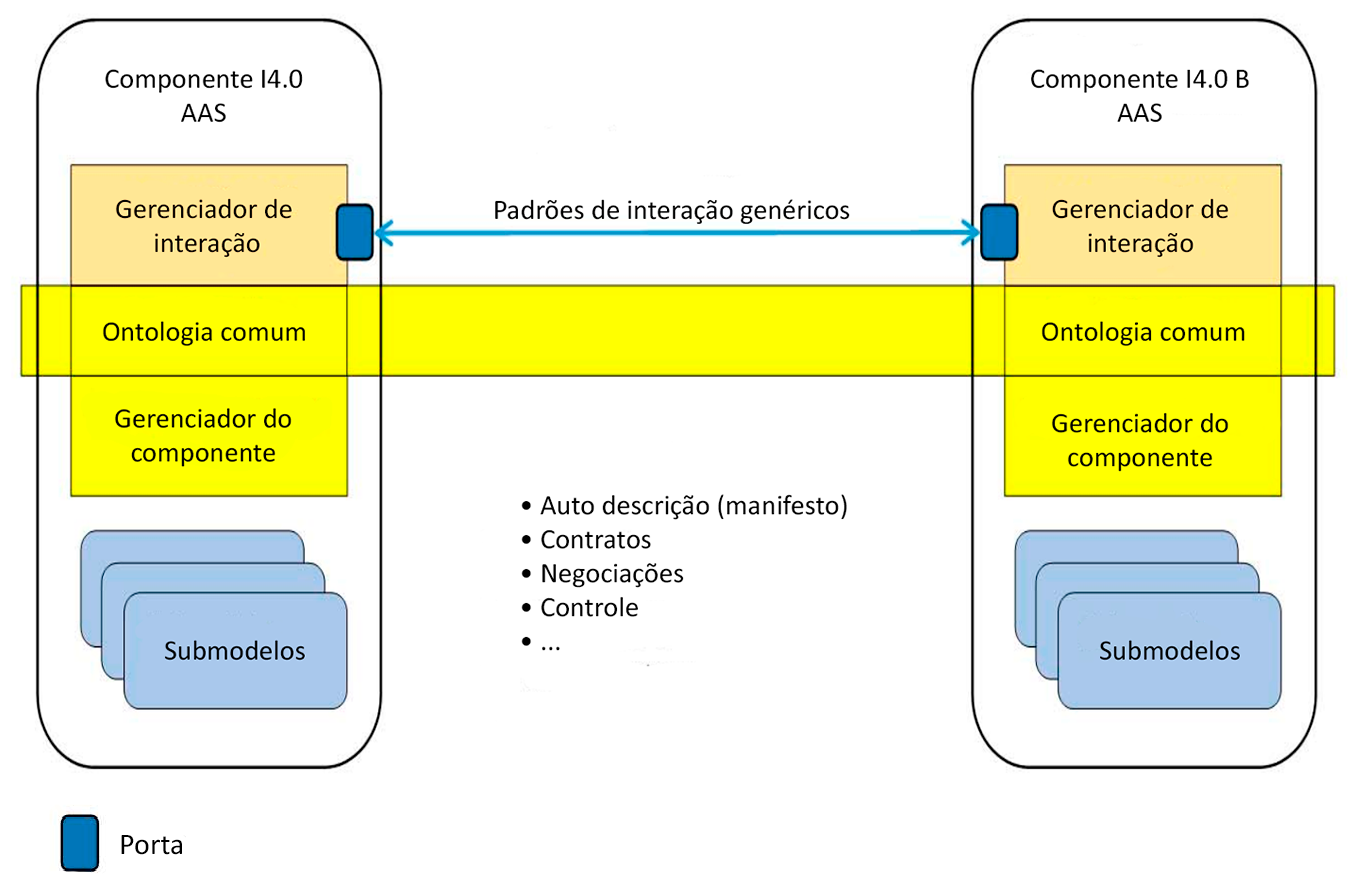
\includegraphics[width=0.8\textwidth]{aas-conexao.png}
		\fonte{\citeonline{marcon2018asset} (adaptado).}
	\end{figure}

	Dentro da I4.0, todos os ativos possuem um AAS com capacidade de comunicação com outros dispositivos. O conjunto Ativo-AAS, que é o objeto real encapsulado pelo \textit{Asset Administration Shell}, é denominado ``Componente I4.0''.
	
	A integração dos ativos, representada pelos Componentes I4.0, em um nível funcional requer uma descrição padronizada das funções (ou capacidades) dos ativos em questão. A padronização de submodelos para descrever detalhadamente cada função pode ser usada para definir requisitos para a fabricação de produtos \cite{bedenbender2017aasexamples}. A \autoref{fig:submodelos} mostra um exemplo de detalhamento de funções sobre um ativo.
	
	\begin{figure}[htb]
		\centering
		\caption{Detalhamento de funções no AAS por meio de submodelos.}
		\label{fig:submodelos}
		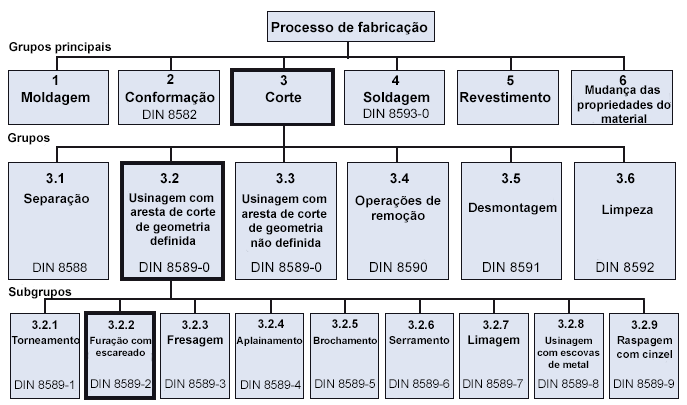
\includegraphics[width=0.85\textwidth]{submodelos.png}
		\fonte{\citeonline{bedenbender2017aasexamples} (adaptado).}
	\end{figure}

	No ambiente de manufatura baseado na I4.0, o produto descreve os requerimentos necessários para sua fabricação e então esses requerimentos são comparados com as descrições da funções das máquinas disponíveis. Portanto, a seleção de um ativo é otimizada, baseando-se nos requerimentos do produto e nas descrições das funções dos ativos.
	
	\section{Logística \& Cadeia de Suprimentos}
	
	A logística é o processo de planejamento, implantação e controle do fluxo eficiente e eficaz de mercadorias, serviços e das informações relativas desde o ponto de origem até o ponto de consumo com o propósito de atender as exigências dos clientes \cite{cscmp2013supplychainglossary}. Essa definição sugere a logística como um processo, o que significa que inclui todas as atividades importantes para a disponibilização de bens e serviços aos consumidores quando e onde estes quiserem adquiri-los \cite{ballou2006cadeiasuprimentos}.
	
	A logística é a essência do comércio \cite{ballou2006cadeiasuprimentos}, ela contribui para que pessoas não mais sejam obrigadas a viver perto das fontes de produção e possam trocar informações e mercadorias com outras regiões de forma efetiva, contribuindo decisivamente para melhorar o padrão econômico de vida geral. 
	
	A logística moderna envolve primariamente o compartilhamento de dados. A logística da informação lida com o fluxo de informações entre humanos e/ou máquinas dentro ou entre organizações \cite{haftor2009information}, que se agrupam formando uma rede de criação de valor por meio de informações. A Logística da Informação é intrinsecamente relacionada a processos de gestão da informação e tecnologias de informação.
	
	A cadeia de suprimentos (CS), por outro lado, é um conceito mais amplo. A CS é onde a logística é exercida. São as partes necessárias para se dar suporte ao pedido de um cliente, desde o produtor até o consumidor final. A gestão da cadeia de suprimentos tem como alvo a orquestração de todas as partes envolvidas por meio de uma logística integrada de forma a se otimizar ao máximo o processo de fornecimento de um produto, serviço ou informação.
	
	A ideia de uma CS simples envolve fornecedor, produtor e cliente \cite{hugos2018supplychain}, porém conceitos modernos ampliam a noção de CS para uma cadeia de suprimentos estendida, que inclui diversos outros fornecedores de serviços em áreas como logística, finanças, \textit{marketing} e desenvolvimento; que, mediante coordenação e colaboração, criam oportunidades para melhoria dos custos ou serviços ao consumidor. A \autoref{fig:cadeia-de-suprimentos} exemplifica a inter-relação das partes em uma cadeia de suprimentos estendida.
	
	\begin{figure}[htb]
		\centering
		\caption{Exemplo de cadeia de suprimentos estendida.}
		\label{fig:cadeia-de-suprimentos}
		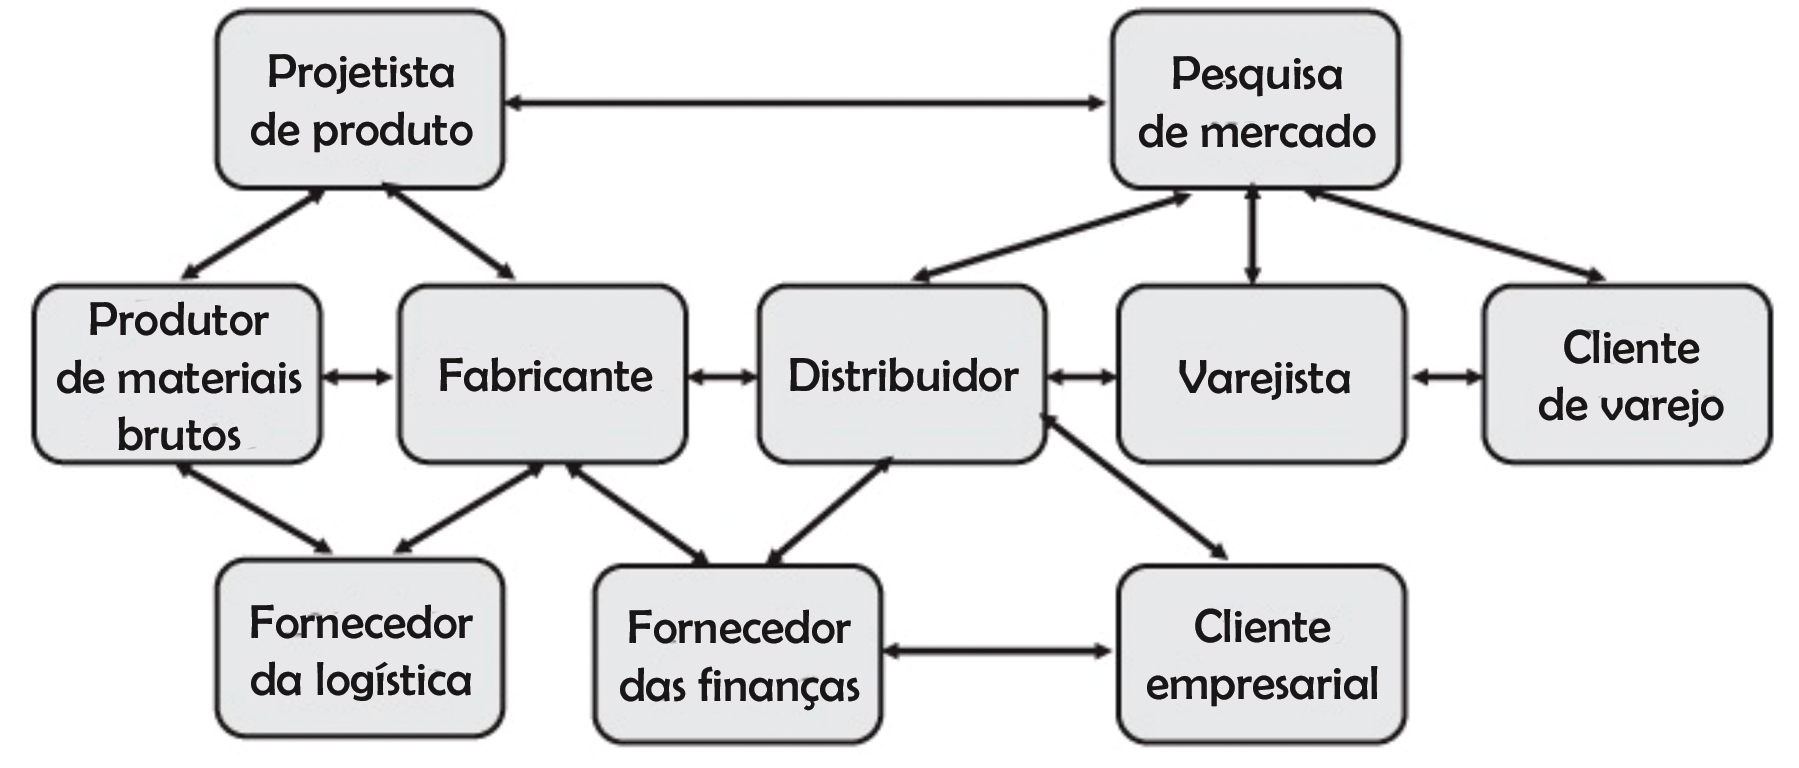
\includegraphics[width=1\textwidth]{cadeia-de-suprimentos.png}
		\fonte{\citeonline{hugos2018supplychain} (adaptado).}
	\end{figure}
	
	Além do eficiente fluxo de materiais e produtos dentro da CS, é imprescindível a manutenção de um canal para troca de informações entre as partes em uma CS, pois sem uma adequada comunicação, gerentes podem acidentalmente tomar decisões supostamente racionais, porém que afetam negativamente outros líderes da cadeia, como o efeito chicote \cite{lee1997bullwhip}, que é a distorção da percepção da procura de um produto que vai se ampliando ao longo da cadeia de suprimentos. Erros de comunicação desse tipo podem acarretar problemas como o aumento do custo de transporte, o elevado tempo de aprovisionamento ao cliente e o desgaste no relacionamento com os fornecedores.
	
	Ao longo da cadeia de suprimentos pode-se observar processos que agregam valor ao produto em desenvolvimento. As etapas de transformação do produto com adição de valor ao longo da CS também podem ser definidas como cadeia de valor.
	
	Uma cadeia de valor (CV) é um conjunto de atividades que empresas de um setor específico desempenham a fim de entregar um produto ou serviço que tenha algum valor perceptível para o mercado \cite{porter1985competitiveadvantage}. A ideia da CV é baseada na agregação de valor ao produto a cada processo de transformação ocorrido, processo esse que envolve a aquisição e consumo de recursos (mão de obra, materiais, equipamentos, instalações, administração, etc). \citeonline{porter1985competitiveadvantage} classifica a CV em duas categorias de atividades que agregam valor ao produto: as atividades primárias e as atividades de apoio (vide \autoref{fig:porter-cadeia-de-valor}).
	
	\begin{figure}[htb]
		\centering
		\caption{Cadeia de valor de Porter.}
		\label{fig:porter-cadeia-de-valor}
		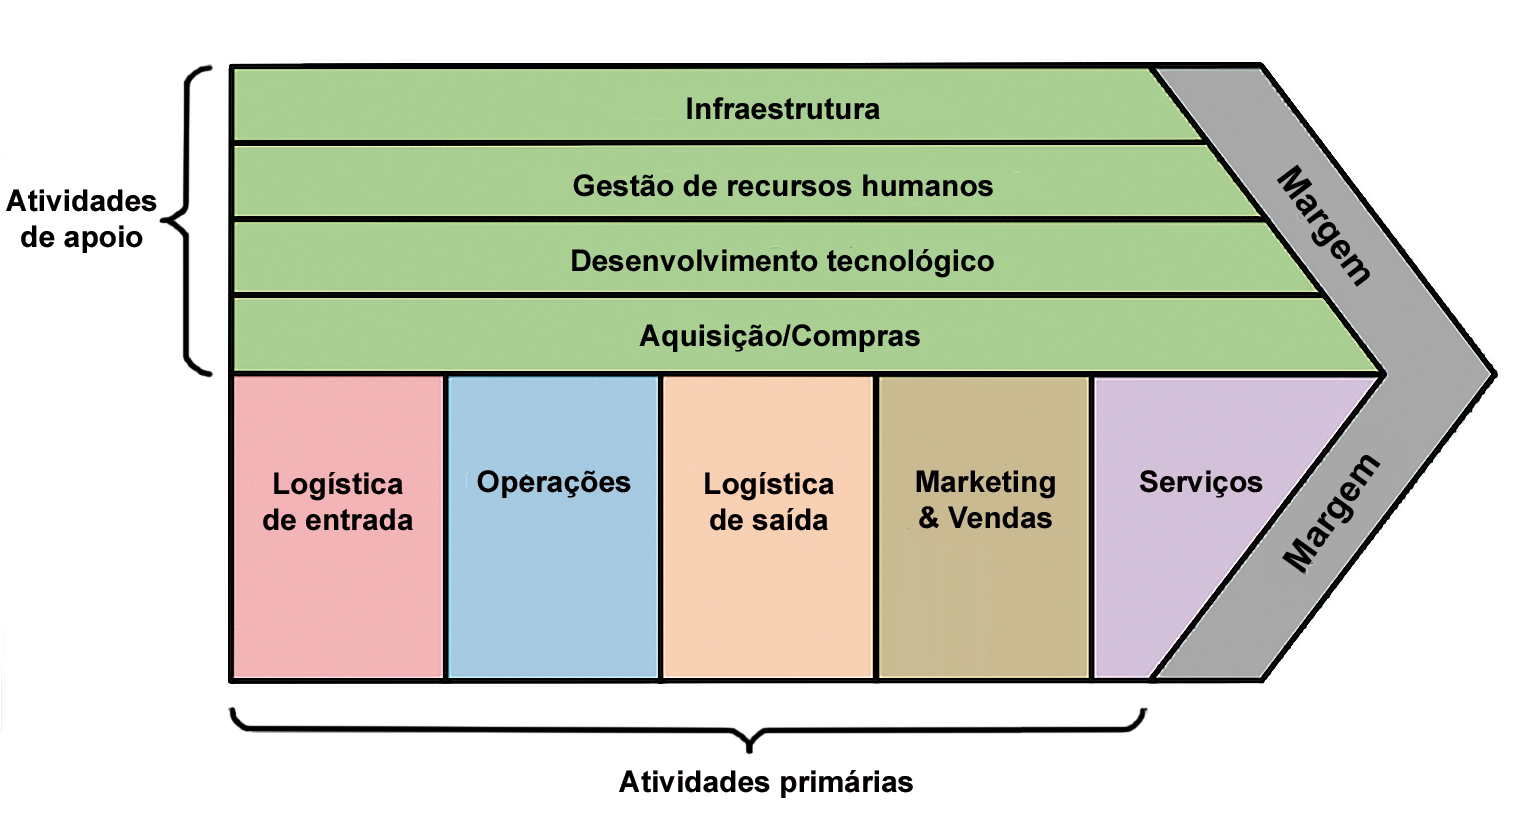
\includegraphics[width=1\textwidth]{porter-cadeia-de-valor.png}
		\fonte{\citeonline{porter1985competitiveadvantage} (adaptado).}
	\end{figure}
	
	As CVs estão focadas em fornecer o máximo valor ao cliente (valor perceptível) com o menor custo e, portanto, é um indicador para a competitividade da empresa. Com o crescente acirramento da competição entre as empresas, essas devem procurar novas formas de agregar mais valor perceptível aos seus produtos, sendo isto em forma de redução de preço, aumento de qualidade, suporte ou qualquer outra nova funcionalidade.
	
	Outra forma de agregação de valor está no princípio de valor compartilhado, que envolve a geração de valor econômico de forma a criar também valor para a sociedade como um todo \cite{porter2011valorcompartilhado} com o enfrentamento de suas necessidades e desafios. Esta necessidade de valor compartilhado parte da percepção generalizada de que empresas prosperam às custas da depreciação da comunidade que as cercam. Soluções que visem o aumento das condições de trabalho, a maior racionalidade e eficiência no tratamento dos recursos naturais necessários para sua atividade e outras formas de balancear o \textit{trade-off} entre eficiência econômica e progresso social são estratégias para se recuperar a legitimidade e a percepção de valor pela sociedade da atividade empresarial.
	
\subsection{Logística 4.0}
	
	Com o entusiasmo acadêmico sobre o tema Indústria 4.0 surgido a partir de 2011, diversas novas linhas de pesquisa derivaram do conceito de I4.0. Uma dessas vertentes é relacionada aos novos desafios tecnológicos na logística e por vezes é denominada ``Logística 4.0''. Estes novos desafios tecnológicos são relacionados primariamente ao intenso uso das Tecnologias de Informação e Comunicação (TIC) e de Internet das Coisas Industrial (IIoT) \cite{barreto2017industry}.
	
	A inserção dessas novas tecnologias ao escopo de estudo da logística acarreta em novos desafios como a alta necessidade de transparência dos processos (visibilidade ao longo da cadeia de suprimentos) e o controle de integridade (produtos certos, no tempo, lugar, quantidade, condição e preço certos) \cite{barreto2017industry}.

	Cadeias de suprimentos atuais podem ser extremamente grandes e complexas (alta interdependência entre as partes) e, portanto, sem uma correta gestão, podem levar à tomada de decisões não ótimas por parte dos gestores humanos. Por estes aspectos, este setor pode ser um dos primeiros a se adaptar a esta nova forma de organização da Indústria 4.0 (ou da Logística 4.0), tornando os processos cada vez mais automatizados para atender a este nova forma de organização.

	Dentro da CS, identificadores individuais podem ser usados a fim de se implementar a conectividade de objetos e informações requeridos no contexto da I4.0. 
	
	A tecnologia de RFID (\textit{Radio-Frequency IDentification}) permite criar uma identificação única para um objeto, onde a etiqueta RFID é um pequeno \textit{chip} que pode ser acoplado e incorporado a um produto e assim armazena um código de identificação único, assim como outras informações relevantes, que podem ser transmitidas sem fio via rádiofrequência. O RFID se mostra como uma alternativa ao tradicional código de barras e o \textit{QR code}. A utilização de identificadores individuais é comum para aplicação de conceitos da I4.0 \cite{alyahya2016rfidwarehousing, vlachos2014rfidimpact, fan2015inventory, bibi2017rfidfood}, pois permite a identificação de cada coisa na rede e possibilita a troca de informações autônomas.
	
	A Logística 4.0, portanto, estabelece uma série de paradigmas que empresas atuando no ramo logístico deverão seguir nos próximos anos para se manterem competitivas. Conceitos de operação como o intercâmbio de informações instantâneas, soluções automatizadas e análise de dados em tempo real abrem caminhos para novos modelos de negócios \cite{strandhagen2017logistics}, que se tornarão essenciais na eficiência em logística moderna.

	
	\section{Ciclo de vida do produto}
	
	O conceito de ciclo de vida do produto foi elaborado em meados da década de 1960 com o propósito de criar um modelo que fosse capaz de explicar o sucesso ou fracasso de um produto introduzido no mercado, sendo capaz também de identificar momentos certos para modificar estratégias de preço, fabricação e quando o produto deve ser descontinuado \cite{cao2012lifecycle}. O modelo inicialmente desenvolvido por \citeonline{levitt1965lifecycle} mostra o padrão de produtos na história passando por quatro estágios bem definidos: Desenvolvimento de mercado, crescimento, maturidade e declínio, conforme observado na \autoref{fig:product-life-cycle}.
	
	\begin{figure}[htb]
		\centering
		\caption{Estágios do ciclo de vida do produto.}
		\label{fig:product-life-cycle}
		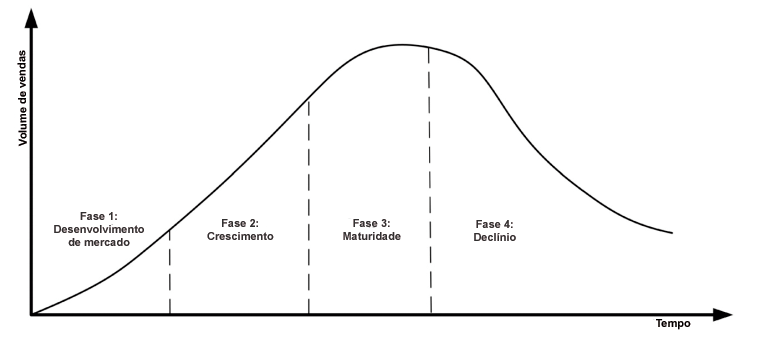
\includegraphics[width=1\textwidth]{product-life-cycle.png}
		\fonte{\citeonline{levitt1965lifecycle} (adaptado).}
	\end{figure}
	
	Vista a tendência global de redução do ciclo de vida do produto devida a rápida taxa de introdução de novas tecnologias para satisfazer a demanda dos clientes, especialmente no mercado de produtos eletrônicos \cite{trappey2008lifecycle}, novas versões de modelos de ciclo de vida do produto vêm sendo elaboradas considerando outros aspectos de mercado e não somente sob a visão da área de \textit{Marketing}. Por vezes, estudos recentes envolvendo ciclo de vida são denominados ``engenharia do ciclo de vida do produto'' (E-CVP) \cite{cao2012lifecycle} e levam em consideração fatores não abordados nos modelos originais como, por exemplo, a fase de pesquisa e desenvolvimento, a retroalimentação de dados, assim como o descarte e reciclagem do produto. Sempre tendo como objetivo auxiliar na tomada de decisões para o sucesso de um produto no mercado.
	
	A \autoref{fig:life-cycle-extension} mostra um modelo de ciclo de vida do produto com elementos que incluem a fase de desenvolvimento e a renovação do produto. A renovação do produto e a decorrente extensão de sua vida é essencial, pois mantém o produto no mercado na forma de novas versões e, assim, amplia as receitas mediante ações estratégicas para agregação de valor. O modelo do ciclo de vida e os elementos presentes sempre irão variar conforme a natureza do produto e tipo de mercado consumidor onde o mesmo está inserido.
	
	\begin{figure}[htb]
		\centering
		\caption{Modelo de ciclo de vida do produto com renovação do produto.}
		\label{fig:life-cycle-extension}
		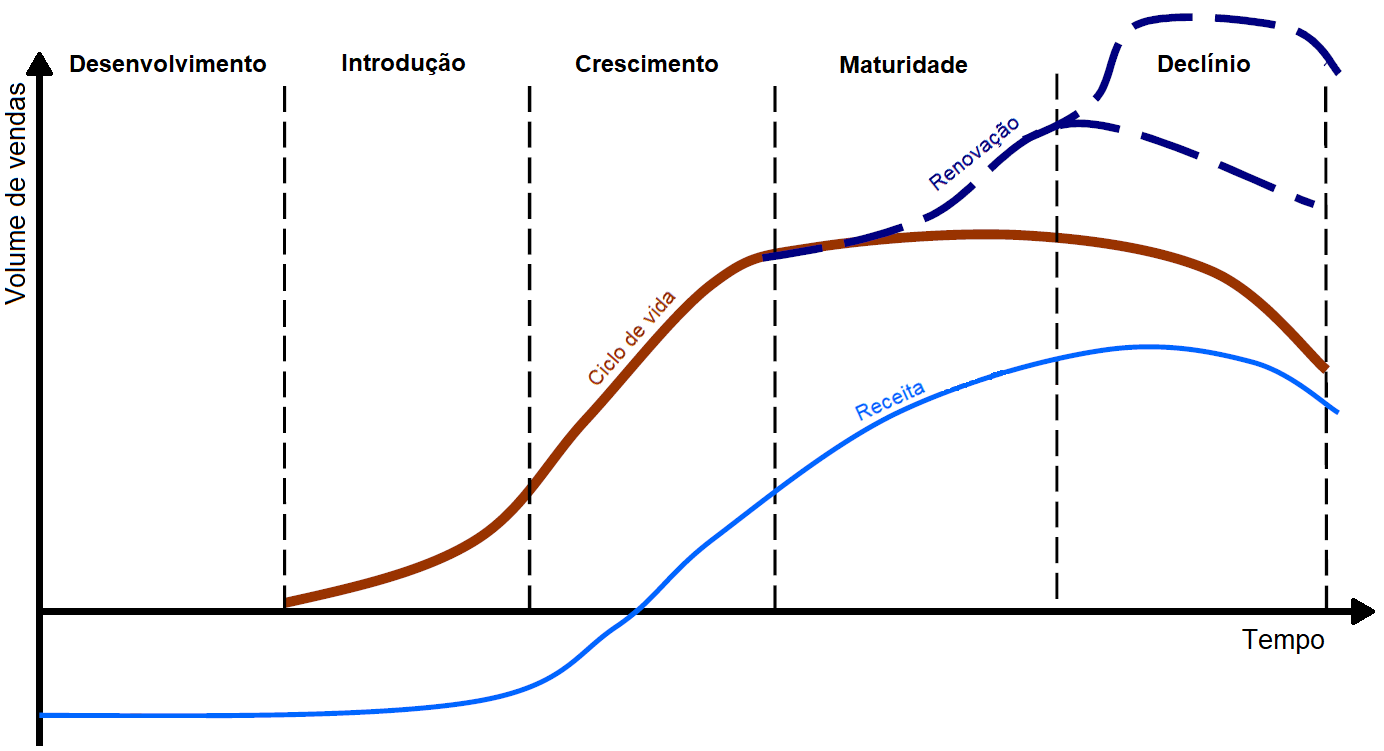
\includegraphics[width=1\textwidth]{life-cycle-extension.png}
		\fonte{\citeonline{liu2010marketingrisk} (adaptado).}
	\end{figure}
	

	
	A gestão do ciclo de ciclo de vida do produto (GCVP) refere-se ao gerenciamento de um ativo ao longo dos estágios típicos de sua vida útil (vide \autoref{fig:product-life-cycle}). Esta gestão dentro dos estágios mencionados pode se referir, por exemplo, à fabricação, comercialização, uso ou qualquer outra fase do ciclo de vida em que o produto se encontra. 
	
	A GCVP tem como finalidade auxiliar gestores na tomada de decisões de negócios por meio de estratégias como políticas de preços, expansão de mercado, retirada do produto ou inserção de novas versões, etc. A função de um GCVP não é gerenciar apenas um de seus produtos, mas gerenciar de maneira integrada todas as suas partes assim como o portfólio de produtos da empresa \cite{stark2015lifecycle}.
	
	Em nível mais alto, o objetivo do GCVP é aumentar as receitas do produto, reduzir os custos relacionados ao produto, maximizar o valor do portfólio de produtos e maximizar o valor dos produtos atuais e futuros para clientes e acionistas \cite{stark2015lifecycle}.
	
	Mais recentemente, novas propostas de modificações de processos industriais por meio da GCVP aparecem como formas de se agregar mais valor ao produto/serviço considerando os ciclos de vida do produto cada vez mais curtos. A Indústria 4.0 e a Logística 4.0 surgem com novas formas de abordagem da gestão do ciclo de vida do produto, considerando as mais modernas necessidades do produto e de seus respectivos clientes.

\section{Memória digital do produto}

	O termo ``Memória Digital do Produto'' (MDP) surgiu pela primeira vez em 2007 por meio de um boletim de notícias de tecnologia de uma empresa alemã fabricante de conectores elétricos e eletrônicos \cite{wahlster2007digitalmemory}. À época, o termo foi tratado com analogia a um diário, que mantinha todas as informações do produto ao longo de seu ciclo de vida.
	
	Hoje, o conceito na literatura se refere a sistemas que permitem a coleta de dados em todas as fases do ciclo de vida do produto para a distribuição e/ou análise. Os dados de interesse do produto podem ser relativos a qualquer fase do produto ao longo de sua cadeia de suprimentos, o que abrange dados de produção individual, de montagem, de distribuição, de uso por parte do consumidor, etc. A \autoref{fig:MDP-ideia} ilustra o conceito de MDP.
	
	\begin{figure}[htb]
		\centering
		\caption{Coleta de dados do produto ao longo da cadeia de valores.}
		\label{fig:MDP-ideia}
		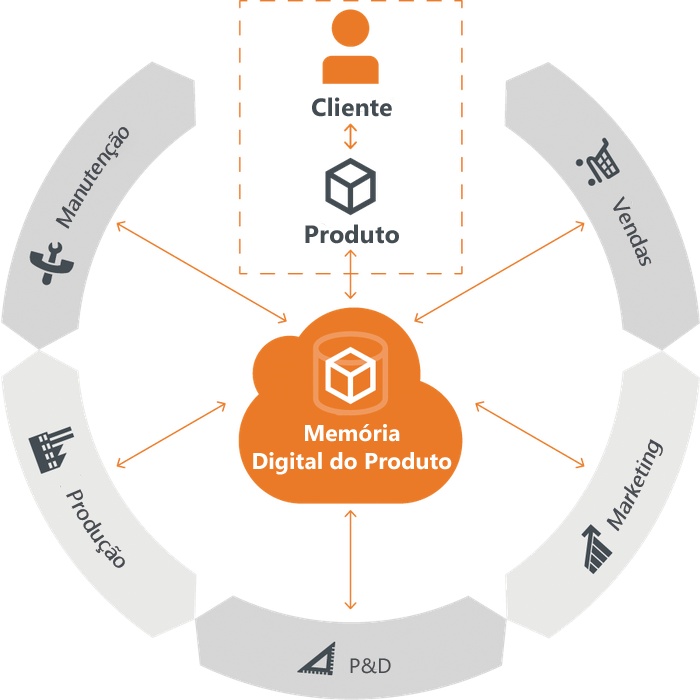
\includegraphics[width=0.6\textwidth]{MDP-ideia.png}
		\fonte{\citeonline{zuhlke2020digitalmemory} (adaptado).}
	\end{figure}
	
	Sua relevância está no fato da tendência de produtos novos apresentarem ciclos de vida cada vez mais curtos e devido ao fato das cadeias de suprimentos apresentarem redes cada vez mais complexas, com múltiplos fornecedores e clientes. Com isso, a MDP manteria registros digitais do ciclo de vida dos produtos, faria o monitoramento constante do seu estado atual e realizaria o rastreamento de sua posição. Segundo \citeonline{wahlster2007digitalmemory}, o acesso a essas informações pelas partes interessadas seria de vital importância na competitividade de empresa produtoras e de comércio, além de abrir novas proteções em relação à pirataria.
	
	Os produtos que são produzidos no cenário de Indústria 4.0 podem ser equipados com a MDP e por meio dela extrair e armazenar informações relevantes de eventos ocorridos ao longo do ciclo de vida do produto a fim de fornecer serviços a todo o ambiente com o qual o produto se relaciona \cite{brandherm2011productmemory}. A MDP fornece também uma forma de rastreabilidade, uma vez que pode armazenar informações geoespaciais do ativo ao longo do tempo.
	
	Implementações de uma memória com informações sobre produto ao longo de sua cadeia de suprimentos é importante, pois torna possível acessar e utilizar informações do mundo real providenciada por diferentes fontes para o potencial benefício das partes interessadas naquele produto \cite{brandherm2011productmemory}, como, por exemplo, fabricantes, transportadores, varejistas e consumidores. E também no pós-venda, onde a MDP continua a ser disponibilizada e ativa, dando a possibilidade ao consumidor de ainda manter contato com cada elo da cadeia de suprimentos e se beneficiar de serviços individuais que se acumulam na memória \cite{brandherm2011productmemory}.
	
\section{Arquitetura orientada a serviços}
	
	Arquitetura Orientada a Serviços (SOA) é um estilo de projeto de \textit{software} em que serviços são disponibilizados a outros sistemas por meio de um protocolo de comunicação comum em uma rede \cite{bell2008soa}. Um serviço é uma unidade de funcionalidade que pode ser fornecida/acessada remotamente. A SOA se destina a ser independente de fornecedores, produtos e tecnologias.
	
	Para quem consome um serviço, a abordagem é como uma caixa preta, o que significa que o consumidor não sabe ou não precisa estar ciente do funcionamento interno deste serviço, sendo apenas o seu resultado relevante. Os serviços representam uma lógica de fornecimento de resultados. É uma abstração de problemas, ou seja, toda a complexidade interna inerente aos serviços pode ser abstraída/desconsiderada pelo consumidores dos serviços.
	
	Dentro do mundo da Indústria 4.0 e de sistemas produtivos, a SOA é uma abordagem que traz novas perspectivas uma vez que se estabelece um conjunto de princípios para uma arquitetura de sistema autônomo e interoperável \cite{candido2009soa}, que tem por objetivo aumentar a eficiência, agilidade e produtividade de um sistema por meio da adoção generalizada do conceito de serviços \cite{souit2013soa}.
	
	Os serviços dentro do ambiente de manufatura encapsulam as funcionalidades necessárias, ocultando todas as heterogeneidades das partes do sistema, permitindo, desta forma, características de flexibilidade, confiabilidade e fácil implementação de	soluções \cite{groba2008soa}.
	
	A SOA dentro do meio industrial permite que um sistema atue como \textit{Middleware}, ou seja, uma camada ou componente de \textit{software} que integra os diferentes aplicativos em um sistema. A \autoref{fig:middleware} ilustra como se dá a interconexão entre os elementos do sistema com e sem um \textit{middleware}.
	
	\begin{figure}[htb]
		\centering
		\caption{Interconexão entre os elementos do sistema com e sem um \textit{middleware}.}
		\label{fig:middleware}
		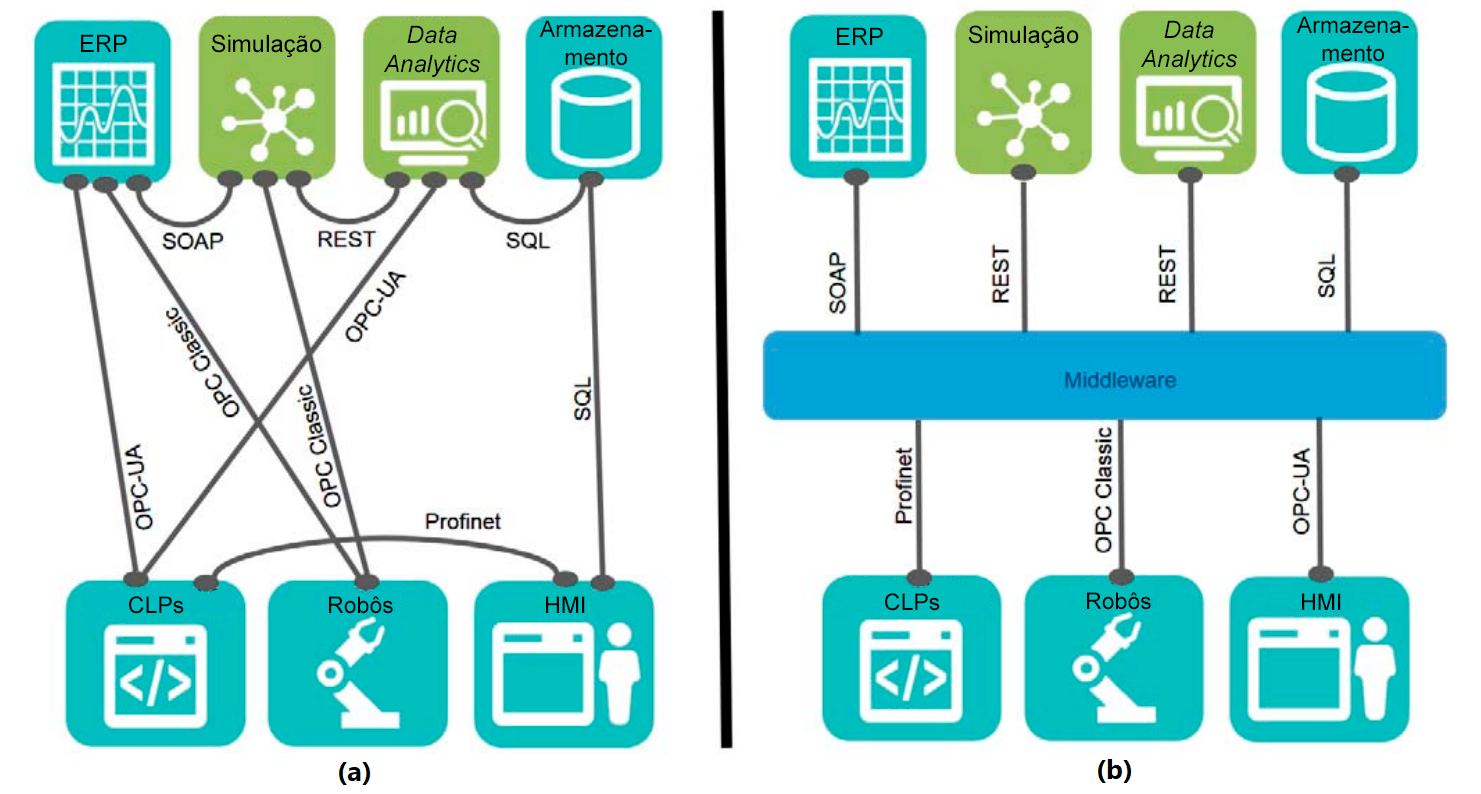
\includegraphics[width=0.9\textwidth]{middleware.png}
		\fonte{\citeonline{gosewehr2017middleware} (adaptado).}
	\end{figure}

	SOA está relacionado à ideia de uma Interface de Programação de Aplicação (\textit{Application Programming Interface} - API), que é o conjunto de rotinas e padrões estabelecidos por um \textit{software} para a utilização das suas funcionalidades por aplicativos externos.
	
	Para se disponibilizar um serviço por meio de uma API, o conceito de \textit{Web Services} (WS) é vastamente utilizado \cite{souit2013soa}. Os WSs podem ser vistos como um conceito padrão para facilitar a interoperabilidade, integração e reuso dos componentes de aplicações.
	
	\subsection{Web Services}
	
	Um \textit{Web Service} (WS) é uma interface que descreve uma série de operações acessíveis por meio de uma linguagem de descrição de serviços padronizada \cite{gottschalk2002webservices}. Um WS executa uma tarefa específica ou um conjunto de tarefas e retorna ao usuário o resultado da operação. Cada aplicação pode ter a sua própria linguagem, que é traduzida para uma linguagem comum, como um XML, JSON, CSV, etc.
	
	Por meio de WSs, as aplicações podem ser descritas, publicadas, localizadas e invocadas em uma rede de comunicação tipo WWW (\textit{World Wide Web}) \cite{souit2013soa}.
	
	A arquitetura de um WS é constituída por três atores básicos: o provedor de serviços, o repositório de serviços e o solicitante de serviços; e por três operações básicas: a publicação, a procura e a interação \cite{gottschalk2002webservices}. A \autoref{fig:componentes-webservice} ilustra os atores e a interação entre eles por meio das operações.
	
	Detalhadamente, os atores em um WS são:
	
	\begin{itemize}
		\item \textbf{Provedor de serviços}: Representa a plataforma que hospeda e fornece um determinado serviço, esta plataforma permite que clientes solicitem serviços e recebam suas respectivas respostas. O provedor de serviços é responsável também por fornecer uma descrição sobre o serviço prestado e publicar esta descrição em um repositório acessível pelo solicitante.
		
		\item \textbf{Repositório de serviços}: É uma plataforma acessível com a função de armazenar e fornecer a descrição sobre diversos WSs. Os WSs são descobertos pelo solicitante por meio do repositório para que assim possa decidir o serviço que melhor o atenda.
		
		\item \textbf{Solicitante de serviços}: É o ator que necessita de um determinado serviço e requisita a sua execução. O solicitante de serviço pode ser uma pessoa acessando um navegador ou uma aplicação realizando solicitações por meio de APIs.		
	\end{itemize}

	\begin{figure}[htb]
		\centering
		\caption{Componentes de um WS e operações.}
		\label{fig:componentes-webservice}
		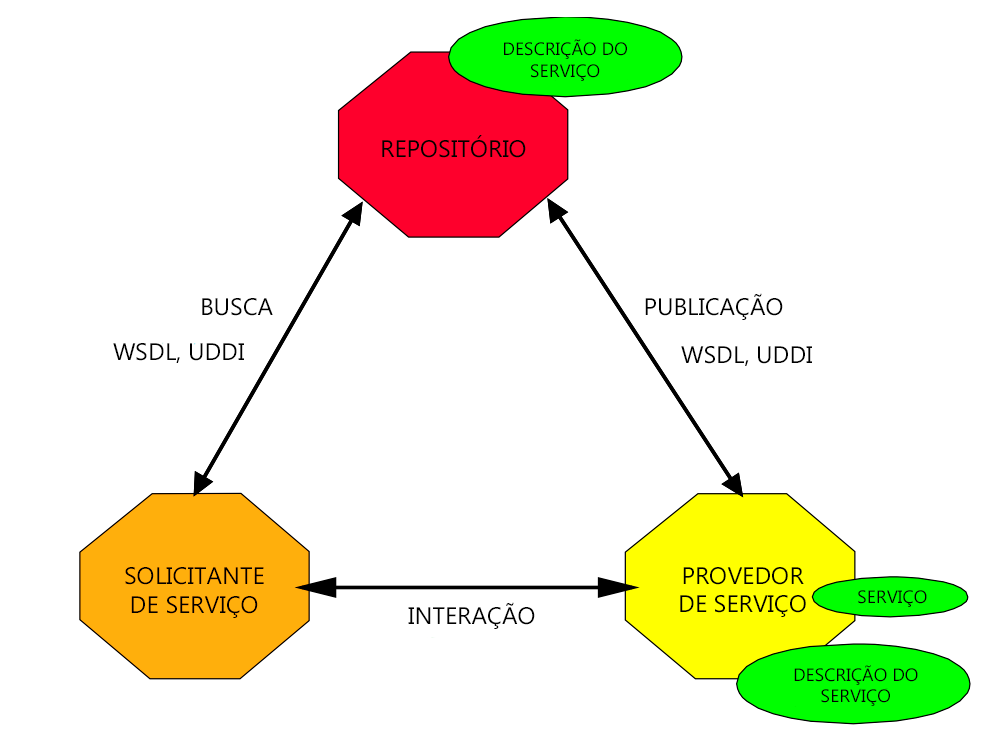
\includegraphics[width=0.8\textwidth]{componentes-webservice}
		\fonte{\citeonline{kreger2001webservices} (adaptado).}
	\end{figure}
	
	Já as operações básicas em WS em detalhe são:
	
	\begin{itemize}
		\item \textbf{Publicação}: Publicação da descrição do serviço pelo provedor em um repositório para que o serviço se torne acessível ao público e os solicitantes possam localizá-lo.
		
		\item \textbf{Busca}: Busca e recebimento da descrição de um serviço. O solicitante pode receber a descrição do serviço pelo provedor ou por meio do repositório.
		
		\item \textbf{Interação}: Comunicação direta entre solicitante e provedor para o fornecimento de serviços. Nesta fase, o solicitante se decide por um determinado serviço dentre os disponíveis no repositório e inicia uma interação com o provedor por meio de uma API.
	\end{itemize}
	
	As etapas de interação entre as entidades são representadas por meio de diagrama UML na \autoref{fig:uml-webservice}. 
	
	\begin{figure}[htb]
		\centering
		\caption{Diagrama UML com os atores e interações em um WS.}
		\label{fig:uml-webservice}
		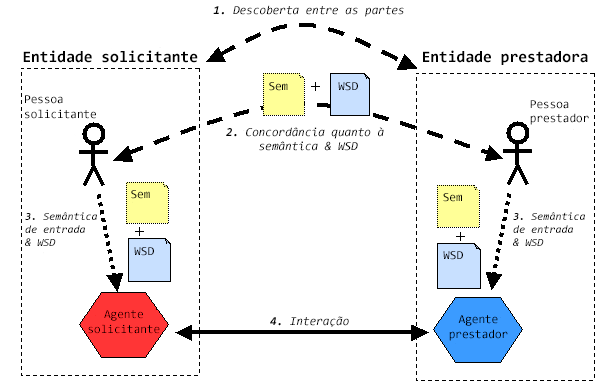
\includegraphics[width=1\textwidth]{uml-webservice}
		\fonte{\citeonline{booth2004webservice} (adaptado).}
	\end{figure}

	Neste diagrama, a Semântica e a Descrição do Web Service (\textit{Web Service Description} -- WSD) representam os documentos com os quais ambas as partes devem concordar para que haja o efetivo fornecimento e consumo do serviço.
	
	O WSD define os formatos de mensagem, tipos de dados, protocolos de transporte e formatos de troca de dados que devem ser usados entre o solicitante e o provedor \cite{booth2004webservice}. O WSD representa um acordo que rege a mecânica de interação com esse serviço. Já a Semântica de um WS é o documento que compartilha o comportamento esperado de resposta deste serviço, pode ser explícito ou implícito, oral ou escrito, processável por máquina ou orientado a humanos, e pode ser um acordo legal ou um acordo informal \cite{booth2004webservice}.

	Os WSs se tornaram bastante atrativos, pois esse modelo pode ser aplicado com tecnologias acessíveis ao solicitante, em particular XML e HTTP, que podem ser acessadas pela maioria dos navegadores convencionais. A disponibilização de serviços interativos na \textit{Internet} se tornou muito popular e com isso surgem novos modelos de negócios como o SaaS (\textit{Software as a Service}), PaaS (\textit{Platform as a Service}), IaaS (\textit{Infrastructure as a Service}), etc.
	
	Dentro do mundo da Indústria 4.0 não é diferente. Ativos podem publicar suas funcionalidades em repositórios e executarem determinadas tarefas mediante solicitação por parte do solicitante, podendo assim serem classificados como uma manufatura como um serviço (\textit{Manufacturing as a Service}) \cite{annunziata2019maas, nichols2020maas, siepen2019maas}.
	
	\subsection{Transferência Representacional de Estado}
	
	A Transferência Representacional de Estado (\textit{Representational State Transfer} - REST) é uma arquitetura de \textit{software} que define padrões para acesso e disponibilização de \textit{Web Services} (WSs). Os WSs que seguem o padrão REST são denominados \textit{RESTful Services}.
	
	A arquitetura REST possibilita a interoperabilidade entre sistemas na \textit{Internet}, pois permite que os sistemas solicitantes acessem e manipulem representações textuais de recursos usando um conjunto uniforme e predefinido de operações sem estado \cite{ferris2004webservices}.
	
	Quando o HTTP é usado como protocolo de comunicação em um \textit{RESTful Service}, cada método do protocolo recebe um tipo de operação padrão do REST. A \autoref{tab:rest} mostra as possíveis operações e seus métodos HTTP correspondentes, quando este protocolo é utilizado.
	

	\begin{table}[htb]
		\centering
		\footnotesize
		\caption{Possíveis operações em um \textit{RESTful Service}.}
		\label{tab:rest}
		\begin{tabular}{p{2cm}p{2cm}p{8cm}}
			\hline
			\textbf{Operação} &
			\textbf{Método \newline HTTP} &
			\textbf{Resposta} \\[5mm]

			\hline
			Criação &
			POST &
			201 (Criado) \\[5mm]
			
			\hline
			Leitura &
			GET &
			200 (OK), 404 (Não encontrado)  \\[5mm]
			
			\hline
			Atualização &
			PATCH &
			200 (OK), 204 (Sem conteúdo), 404 (Não encontrado),405 (Não permitido) \\[5mm]
			
			
			\hline
			Exclusão &
			DELETE &
			200 (OK), 404 (Não encontrado), 405 (Não permitido) \\[5mm]
			
			\hline
		\end{tabular}
		\fonte{\cite{fielding2000architecture} (adaptado).}
	\end{table}

\chapter{Arquitetura para compartilhamento de informações do ativo}


\section{Estrutura do AAS e seus submodelos}

	O conceito de Memória Digital do Produto (MDP) é inserido dentro da Indústria 4.0 com o objetivo de se agregar valor por meio da possibilidade de acesso a informações sobre o ativo entre parceiros ao longo da cadeia de valor de um ativo.
	
	A MDP na I4.0 é definida como qualquer dado digitalizado que se relacione ao ativo. A MDP é um banco de dados que armazena informações referentes a cada um dos submodelos em um AAS. Cada submodelo agrega informações semelhantes relativas ao ativo. A MDP está localizada no corpo do AAS (\textit{body}).
	
	Os submodelos são divididos em duas categorias, a parte pública e a parte restrita.
	
	Os submodelos públicos contêm informações não confidenciais sobre o ativo e têm funções de identificação na rede. Os submodelos públicos ``Identificação'' e ``Referências'' serão tratados neste trabalho. Estes submodelos têm a função de identificação a si mesmo e criação de \textit{links} com referências para os demais submodelos restritos no AAS e estão localizados no cabeçalho do AAS (\textit{header}).
	
	Os submodelos restritos, por sua vez, contêm informações sensíveis sobre o ativo, que podem ser acessadas mediante autenticação, estes submodelos representam a carga útil do AAS, pois é a porção de informação que é de fato relevante para o cliente que consumirá as informações do AAS. Os submodelos restritos serão mencionados nesse trabalho simplesmente como ``Submodelos''.
	
	A estrutura proposta de um AAS é apresentada na Figura \ref{fig:submodelos-publicos-e-restritos}.
	
	\begin{figure}[H]
		\centering
		\caption{Submodelos públicos e restritos de um AAS.}
		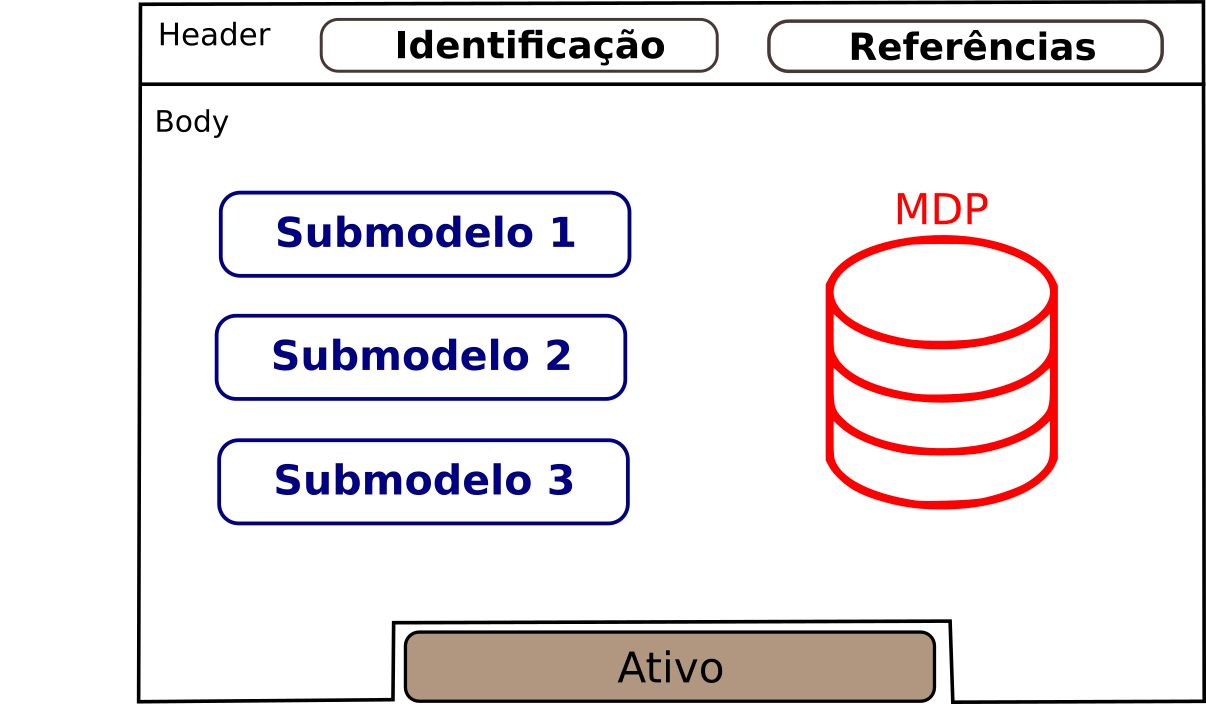
\includegraphics[width=0.7\textwidth]{submodelos-publicos-e-restritos.png}
		\label{fig:submodelos-publicos-e-restritos}
		\source{O autor.}
	\end{figure}

	As informações geradas pelos submodelos são armazenadas na MDP por meio de uma API REST. O acesso à MDP referente a cada submodelo restrito é feito mediante autenticação.
	
	A Tabela \ref{tab:submodelos-publicos-restritos} detalha os tipos de submodelos.
	
	
		\begin{table}[H]
		\centering
		\caption{Caracterização dos submodelos públicos e restritos.}
		\begin{tabular}{|p{1.3in}|p{4in}|}
			
			\hline
			\textbf{Submodelo}
			&\textbf{Descrição} \\
			
			\hline
			Submodelo público
			& Tem a função identificação do ativo na rede. Contém informações que podem ser acessadas sem a necessidade de autenticação, como, por exemplo, seu identificador único universal (UUID - Universal Unique IDentifier), o modelo e fabricante do ativo. O submodelo não tem a função de fornecer uma ficha técnica detalhada, mas apenas uma caracterização abstrata do ativo. Dependendo da confidencialidade do ativo, o submodelo de identificação pode apenas apresentar o UUID como informação pública. Sem o UUID, o AAS se torna inacessível para qualquer uma das partes da cadeia de suprimentos. \\
			
			\hline
			Submodelo restrito
			& Representa a carga útil do AAS (\textit{payload}). Os submodelos restritos contêm as propriedades, funcões e demais regras de negócio do ativo. Os dados dos submodelos são armazenadas na MDP, que podem ser acessada mediante autenticação. Os dados contidos na MDP dos submodelos restritos quando processados fornecem informações sobre o ativo e agregam valor ao mesmo. Além disso, novos modelos de negócio surgem sob os dados gerados pelo ativo. Alguns exemplos de submodelos restritos incluem: a ficha técnica detalhada do ativo, submodelos de histórico de leitura de sensores, histórico de geolocalização do ativo, histórico de padrão de uso, etc.\\
			
		
			\hline
			
		\end{tabular}
		\label{tab:submodelos-publicos-restritos}
		\source{O autor.}
	\end{table}
	
\section{O repositório e a descoberta de AAS's}
	
	Os submodelos \textbf{Identificação} e \textbf{Referências} são a forma primária para a identificação e acesso a um AAS, pois estes submodelos possuem o UUID do AAS e as referências para o acesso dos demais submodelos do AAS.
	
	Para que um AAS seja acessível pelas demais partes da cadeia de suprimentos, os submodelos Identificação e Referências devem estar disponíveis em uma lista pública que contém o submodelo de identificação de todos os AAS disponíveis, esta lista pública é definida como Repositório.
	
	O repositório, além de uma cópia do submodelo de identificação de cada AAS, possui também uma cópia das referências para os demais submodelos de cada AAS, conforme ilustrado na Figura \ref{fig:repositorio}.
	
	
	\begin{figure}[H]
		\centering
		\caption{Repositório com referências aos AAS's.}
		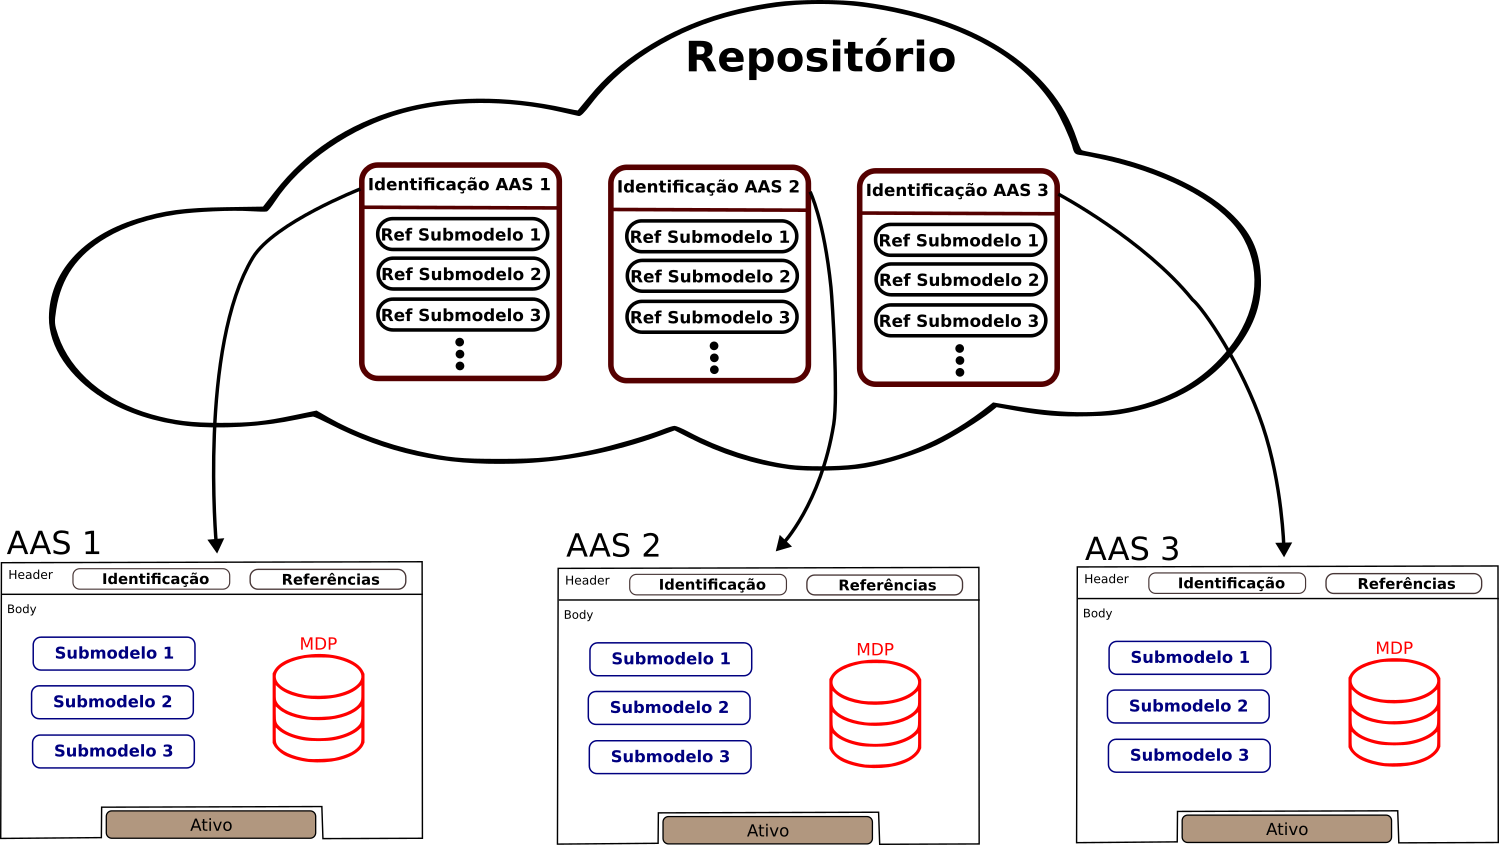
\includegraphics[width=1\textwidth]{repositorio.png}
		\label{fig:repositorio}
		\source{O autor.}
	\end{figure}
	
	O repositório sob contexto da I4.0 é um \textit{web service}, ou seja, um serviço oferecido de um dispositivo eletrônico para outro dispositivo eletrônico com a comunicação entre eles por meio da \textit{World Wide Web} (Internet).
	
	Um \textit{web service} é disponibilizado por meio de um servidor que roda o serviço, escutando e respondendo solicitações de clientes através de uma determinada porta ou rede. Os clientes, por sua vez, consomem o serviço disponibilizado pelo servidor por meio de solicitações.
	
	Para o fornecimento e consumo de \textit{web services} entre cliente e servidor, diversos protocolos de comunicação podem ser utilizados na camada de aplicação do modelo padrão TCP/IP. O protocolo de comunicação para a adoção REST mais difundido na atualidade é o HTTP \cite{gruner2016restful}, porém alguns outros ainda operam, como o MQTT, que está presente principalmente na área de automação residencial e IoT \cite{yokotani2016mqtt}.
	
	
\section{Os quatro elos no compartilhamento de informações na CS}
	
	O modelo estrutural proposto envolve quatro componentes básicos: o AAS, a MDP, o repositório e o cliente. A Figura \ref{fig:4-elos} mostra as conexões entre os quatro elos, onde cada seta representa o fluxo de informações direcional. A interrelação entre as partes envolvendo o servidor REST é detalhada no Capítulo \ref{comunicacao-CS}.
	
	\begin{figure}[H]
		\centering
		\caption{Repositório com referências aos AAS's.}
		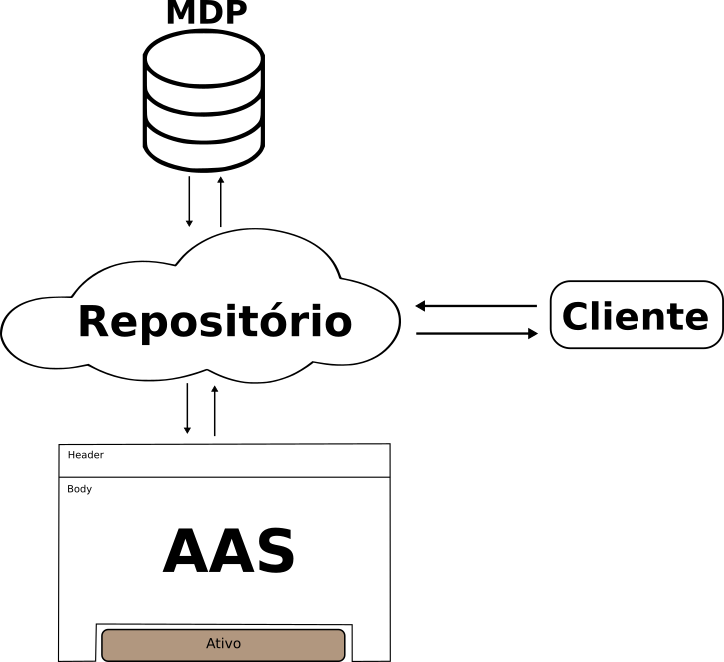
\includegraphics[width=0.8\textwidth]{4-elos.png}
		\label{fig:4-elos}
		\source{O autor.}
	\end{figure}
	
	A MDP é representada neste modelo fora do AAS exclusivamente por fins didáticos. A MDP é parte do AAS. A MDP, entretanto, não estará necessariamente armazenada no escopo físico da empresa, mas oferecida em uma plataforma de serviços de computação em nuvem mais adequada para o armazenamento de grandes quantidades de dados, assim como para uma alta capacidade de requisições.
	
	Os elos necessários para o modelo estrutural de acesso a informações pelas partes da cadeia de suprimentos são detalhados na Tabela \ref{tab:4-elos}.
	
	\begin{table}[H]
		\centering
		\caption{Os quatro elos do modelo estrutural de acesso de informações.}
		\label{tab:4-elos}

			\begin{tabular}{lp{12cm}}
				\hline
				\rowcolor[HTML]{F0F0F0} 
				{\color[HTML]{000000} \textbf{Componente}} 
				& {\color[HTML]{000000} \textbf{Descrição}} \\ \hline
				\rowcolor[HTML]{FFFFFF} 
				{\color[HTML]{000000} AAS}         
				& {\color[HTML]{000000} O AAS é a conexão direta com o ativo, o AAS extrai e disponibiliza informações sobre o ativo. Cada submodelo do AAS representa um conjunto de informações semelhantes e suas respectivas funções de agregação.} \\
				\rowcolor[HTML]{F7F7F7} 
				{\color[HTML]{000000} Cliente}     
				& {\color[HTML]{000000} O cliente é a parte que irá consumir as informações disponibilizadas pelo AAS. O cliente representa cada uma das partes da cadeia de suprimentos, ou seja, o fabricante, o distribuidor, o consumidor, etc. }  \\
				\rowcolor[HTML]{FFFFFF} 
				{\color[HTML]{000000} Repositório}
				& {\color[HTML]{000000} O repositório é o \textit{web service} RESTful que faz a interface entre a MDP e o Cliente, ou entre a MDP e o AAS. O cliente solicita ao repositório operações de consulta ao MDP (Método GET), enquanto que o AAS solicita ao repositório operações de inserção de dados ao MDP (Método POST)}        \\
				\rowcolor[HTML]{F7F7F7} 
				{\color[HTML]{000000} MDP}
				& {\color[HTML]{000000} A memória digital do produto é o banco de dados que armazena todas as informações históricas relativas aos submodelos do AAS. A MDP não precisa necessariamente ser um banco de dados único, mas pode ser distribuído conforme a necessidade e tipo de dados a se armazenar.}       
			\end{tabular}%

	\source{O autor.}
	\end{table}
	
	
	
	
	
\section{Estrutura de dados da MDP}

	Segundo \citeonline{radack2009exchangedata}, a série IEC 61360 fornece uma estrutura e um modelo de informação de dicionários sobre produtos. O conceito de tipo de produto é representado por ``classes'' e as características do produto são representadas por ``propriedades''.

	Tais propriedades são elementos de dados padronizados. As definições de tais propriedades podem ser encontradas em vários repositórios, como IEC CDD (dicionário de dados comuns) ou eCl@ss.
	
	A definição de uma propriedade associa um identificador exclusivo mundial a uma definição, que é um conjunto de atributos bem definidos. Atributos relevantes para o AAS são, entre outros, seu nome, o símbolo, a unidade de medida e uma definição textual legível para humanos da propriedade \cite{bader2019aas}.
	
	A publicação sugere formatos de transferência e armazenamento de dados. É especificado o UML (modelo neutro) e esquemas em XML e JSON, assim como mapeamentos para OPC UA, AutomationML e o \textit{Resource Description Framework} (RDF) \cite{plattform2019detailsaas}.
	
	A estrutura proposta usa o padrão de troca de dados JSON, que utiliza texto legível a humanos, no formato atributo-valor (natureza auto-descritiva). O um modelo de transmissão de informações no formato JSON é muito usado em \textit{web services} que usa transferência de estado representacional (REST) e aplicações AJAX, substituindo o uso do XML.
	
	A estrutura de armazenamento proposta usa banco de dados orientado a documentos que usa document em formato JSON com esquemas pré-definidos.
	
	A Figura \ref{fig:json} mostra um exemplo de estruturação de dados para troca e armazenamento de informações em JSON.
	
	\begin{figure}[H]
		\centering
		\caption{Formato de intercâmbio de informações da MDP em JSON.}
		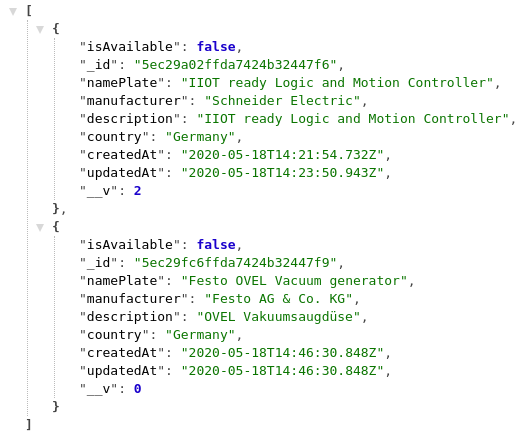
\includegraphics[width=0.8\textwidth]{json.png}
		\label{fig:json}
		\source{O autor.}
  \end{figure}
  

  \section{Acesso à MDP pelo AAS e Cliente}
	\label{comunicacao-CS}
	
	O acesso à MDP pelo AAS a fins de escrita e pelo Cliente a fins de leitura é realizado por meio de uma API REST. No contexto na I4.0, esta API Rest é denominada ``Repositório'' e funciona como uma interface para acesso às funcionalidades do banco de dados da MDP, tais como operações CRUD (criação, leitura, atualização e exclusão).
	
	Além das operações de manipulação da MDP, o repositório serve como uma plataforma de descoberta de AAS's disponíveis, uma vez que ele contém os UUIDs de todos os AAS cadastrados.
	
	
	\subsection{A comunicação AAS - MDP}
	
	A comunicação entre o AAS e a MDP pode ser dividida em cinco etapas:
	
	\begin{enumerate}
		\item O AAS envia ao repositório uma solicitação de inserção de dados sobre o ativo.
		\item O repositório recebe a solicitação de inserção, valida os dados, checa autenticação e envia uma soliciação de inserção de dados à MDP.
		\item A MDP processa as informações e insere em sua estrutura os novos dados.
		\item A MDP retorna uma confirmação de inserção dos dados ao repositório.
		\item O Repositório retorna ao AAS o \textit{status} da solicitação inserção de dados conforme convenções do protocolo HTTP.
	\end{enumerate}
	
	
	A comunicação AAS-MDP é ilustrada na Figura \ref{fig:aas-mdp}.
	
	
	\begin{figure}[H]
		\centering
		\caption{Comunicação AAS-MDP.}
		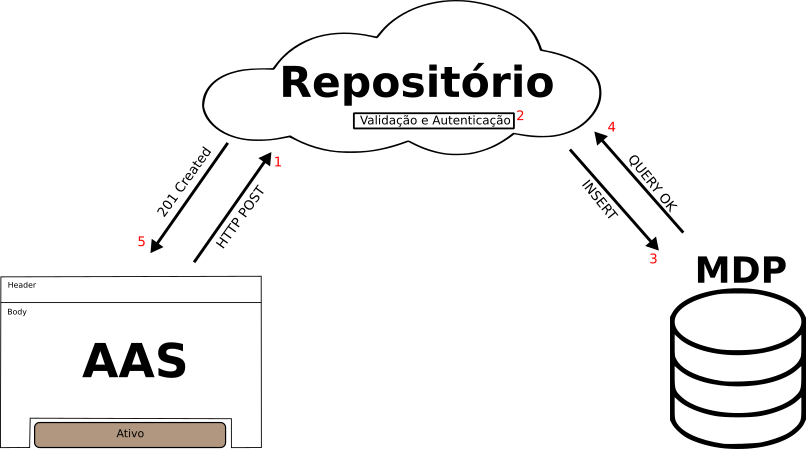
\includegraphics[width=0.8\textwidth]{aas-mdp.png}
		\label{fig:aas-mdp}
		\source{O autor.}
	\end{figure}

	
	\subsection{A comunicação Cliente - MDP}
	
	A comunicação entre o Cliente e a MDP, assim como a comunicação AAS-MDP, pode ser dividida em cinco etapas semelhantes:
	
	\begin{enumerate}
		\item O Cliente membro da cadeia de suprimento envia ao repositório uma solicitação de consulta de dados sobre o ativo.
		\item O repositório recebe a solicitação de consulta, checa autenticações necessárias e envia uma soliciação de consulta à MDP.
		\item A MDP processa as informações solicitadas através de uma consulta do tipo SELECT.
		\item A MDP retorna os dados solicitados ao repositório com uma confirmação de consulta executada com sucesso.
		\item O Repositório retorna ao Cliente os dados solicitados juntamento com o \textit{status} da solicitação de consulta conforme convenções do protocolo HTTP.
	\end{enumerate}
	
	
	A comunicação Cliente-MDP é ilustrada na Figura \ref{fig:cliente-mdp}.
	
	\begin{figure}[H]
		\centering
		\caption{Comunicação Cliente-MDP.}
		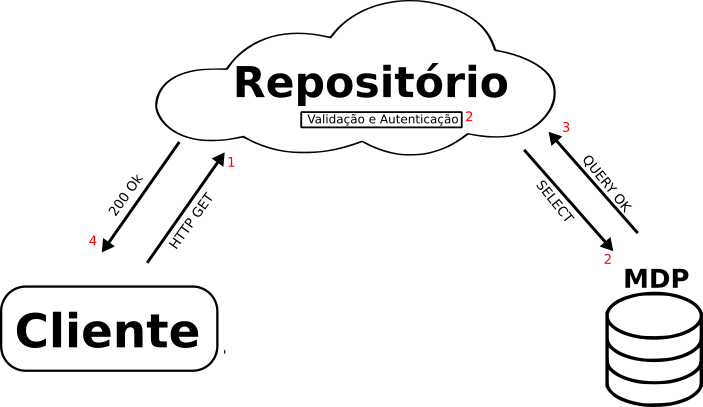
\includegraphics[width=0.8\textwidth]{cliente-mdp.png}
		\label{fig:cliente-mdp}
		\source{O autor.}
	\end{figure}
	
	
	\subsection{Interação AAS-MDP-Cliente}
	
	A interação AAS-MDP-Cliente é basicamente uma operação simultânea assíncrona da comunicação AAS-MDP e a comunicação Cliente-MDP.
	
	Nesta interação, diversos AAS's e diversos clientes podem fazer solicitações independentes ao repositório de operações CRUD.
	
	A Figura \ref{fig:aas-mdp-cliente} ilustra interações simultâneas entre o cliente ou o AAS com o repositório para solicitações de leitura e solicitações de escrita na MDP, respectivamente.
	
	\begin{figure}[H]
		\centering
		\caption{Comunicação Cliente-MDP.}
		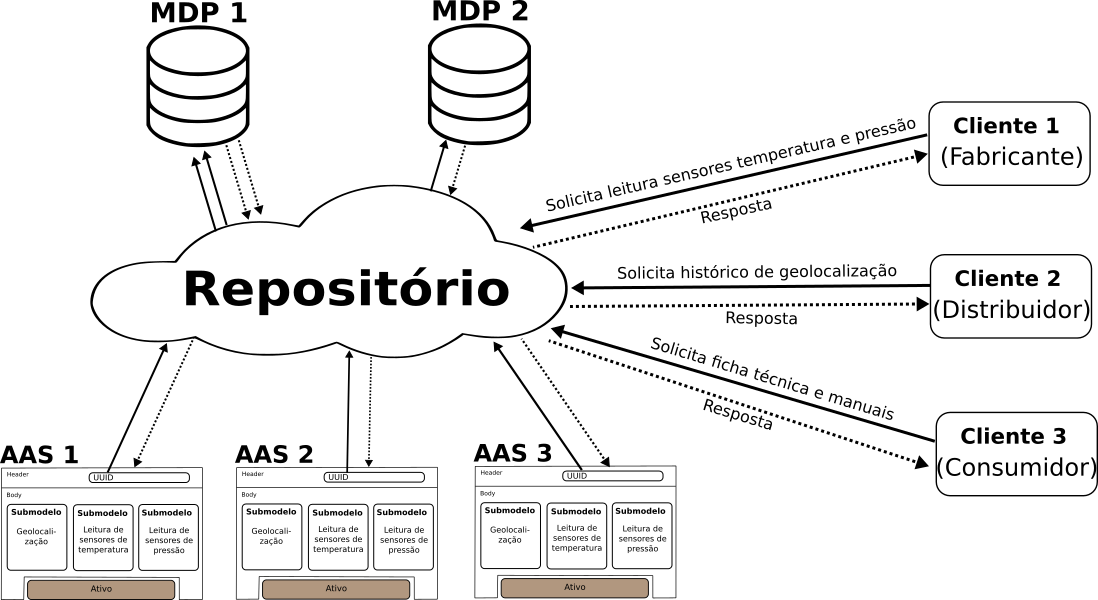
\includegraphics[width=1\textwidth]{aas-mdp-cliente.png}
		\label{fig:aas-mdp-cliente}
		\source{O autor.}
	\end{figure}

	Cada AAS não precisa necessariamente estabelecer conexão com apenas uma MDP, diferentes submodelos de uma AAS podem ter seus dados salvos em diferentes serviços de armazenamento em nuvem, ou até mesmo em um banco de dados local na própria empresa.
	
	Cada cliente deve se autenticar junto ao repositório a fim de ser consultar a MDP. Isto significa que cada cliente não tem o acesso integral a todos os submodelos do AAS, mas somente àquele que for determinado por projeto.
	
	Na Figura \ref{fig:aas-mdp-cliente} são exemplificados três tipos de clientes com seus respectivos escopos de autenticação. O Cliente 1 pode acessar somente informações relativas ao submodelo de leitura de sensores de temperatura e pressão, o Cliente 2 pode acessar somente informações sobre o submodelo de geolocalização, o Cliente 3 acessa somente o submodelo de ficha técnica e manuais.
	
	
	
	\section{O MDP e as Camadas do RAMI4.0}

	Segundo \citeonline{iec2017rami}, o RAMI4.0 fornece uma visão estruturada dos principais elementos de um ativo, usando um modelo de níveis composto por três eixos. Desta forma, interrelações complexas podem ser divididas em seções menores e mais gerenciáveis, combinando os três eixos em cada ponto da vida do ativo para representar cada aspecto relevante.
	
	Desta forma, a coparticipação da MDP deve ser representada também conforme a estrutura do RAMI4.0, explicitando em que parte acontece cada interação entre AAS, MDP, Repositório e Cliente.
	
	
	Desenvolvendo....
\chapter{A MDP e o ciclo de vida do produto}

\section{Distinção de tipo e instância de um ativo}

	O modelo do RAMI4.0 apresenta um eixo de ciclo de vida generalizado, derivado da norma IEC 62890 \cite{adolphs2015rami}. A ideia do trás do eixo Ciclo de Vida e Cadeia de Valor é distinguir todos os ativos na I4.0 entre tipos e instâncias:
	
	\begin{itemize}
	  \item Tipo: Presente desde a concepção/conceitualização até os primeiros protótipos/testes. O ``tipo'' de um ativo é definido e propriedades e funcionalidades distintas são definidas e implementadas. Todos os artefatos de design (interno) são criados, como dados CAD, esquemas, software incorporado e associados ao tipo de ativo. Aumentando a capacidade de produção. As informações 'externas' associadas ao ativo são criadas, como folhas de dados técnicos, informações de marketing. O processo de venda é iniciado.
	  
	  \item Instância: São criadas/produzidas com base nas informações de um tipo de ativo. Informações específicas sobre produção, logística, qualificação e teste estão associadas às instâncias do ativo. Fase de uso pelo comprador das instâncias do ativo. Os dados de uso estão associados à instância do ativo e podem ser compartilhados com outros parceiros da cadeia de valor, como o fabricante da instância do ativo.
	  Também inclui: manutenção, re-design, otimização e desativação da instância do ativo. O histórico completo do ciclo de vida está associado ao ativo e pode ser arquivado / compartilhado para documentação.
	  
	\end{itemize}

	Esse relacionamento deve ser mantido ao longo da vida das instâncias do ativo. Por esse relacionamento, as atualizações nos tipos de ativos podem ser encaminhadas para as instâncias de ativos, automaticamente ou sob demanda \cite{bader2019aas}.
	
	Os relacionamentos entre tipos e instância são cíclicos e possibilitam a retroalimentação de informações. Para os ativos do produto, por exemplo, informações sobre o uso e manutenção de instâncias do produto armazenadas na MDP podem melhorar a fabricação de novos produtos, além de causar melhorias no projeto do próximo tipo de produto.
	
	Portanto, o fluxo de informações entre tipos e instâncias de um produto são essenciais para a melhoria do projeto do produto. A Figura \ref{fig:aas-lifecycle} ilustra como ocorre a instancialização (criação de uma instância a partir de um tipo) e o uso da MDP das instância para a criação de novas versões de um 'tipo'.
	
	\begin{figure}[hbt!]
	  \centering
	  \caption{Ciclo de vida do produto.}
	  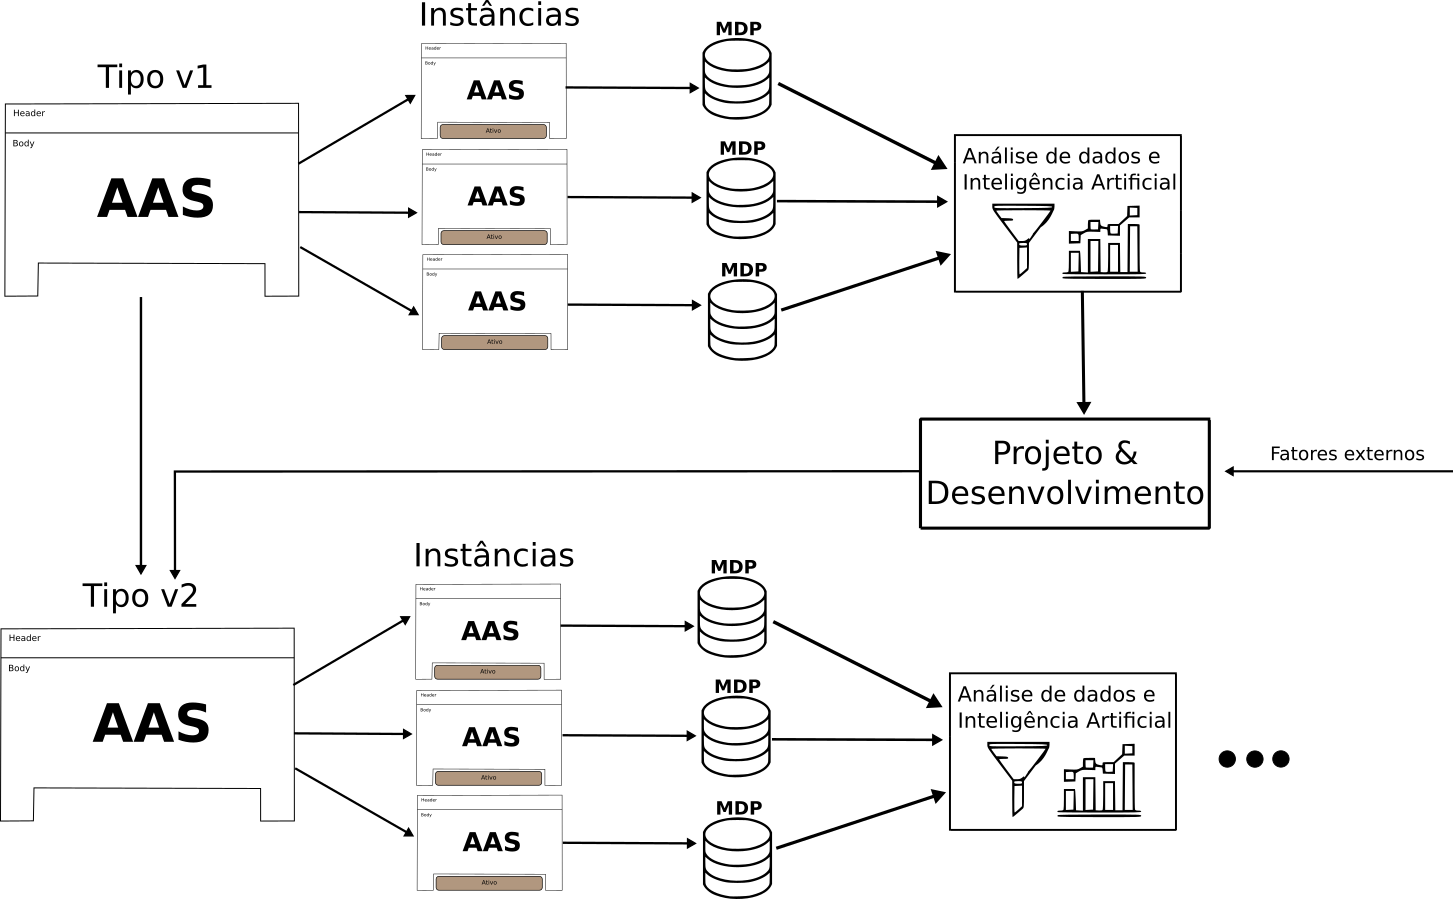
\includegraphics[width=1\textwidth]{aas-lifecycle.png}
	  \label{fig:aas-lifecycle}
	  \source{O autor.}
	\end{figure}


\section{Desenvolvimento do produto orientado a dados}

\lipsum[1-1]

\section{Manutenção do produto orientado a dados}

\lipsum[1-1]
\chapter{Prova de conceito}

	Para o fornecimento e consumo de serviços entre AAS Clientes e Servidores, diversas protocolos e tecnologias podem ser adotadas.
	
	Este capítulo tem o objetivo de apresentar uma implementação funcional da arquitetura apresentada no \autoref{cha:arquitetura} como prova de conceito, adotando alguns protocolos e tecnologias atualmente comuns meio da engenharia de \textit{software} e desenvolvimento de sistemas.
	

\section{ Arquitetura do WS e tecnologias utilizadas }

	O protocolo de comunicação para o fornecimento de WSs mais comumente aplicado atualmente é o HTTP \cite{gruner2016restful}, seguindo as regras de operações padronizadas definidas pelo padrão REST.
	
	Alguns outros protocolos também são aplicados para oferecimentos de WSs, como o MQTT, que está presente principalmente na área de automação residencial e IoT \cite{yokotani2016mqtt}.


\section{ Estruturação dos dados da MDP }

	A estrutura proposta usa o padrão de troca de dados JSON, que utiliza texto legível a humanos, no formato atributo-valor (natureza auto-descritiva). O um modelo de transmissão de informações no formato JSON é muito usado em WSs que usam transferência de estado representacional (REST) e aplicações AJAX, substituindo o uso do XML.
	
	A estrutura de armazenamento implementada usa banco de dados orientado a documentos que usa documento em formato JSON com esquemas pré-definidos.
	
	A \autoref{fig:json} mostra um exemplo de estruturação de dados para troca e armazenamento de informações em JSON.
	
	\begin{figure}[htb]
		\centering
		\caption{Formato de intercâmbio de informações da MDP em JSON.}
		\label{fig:json}
		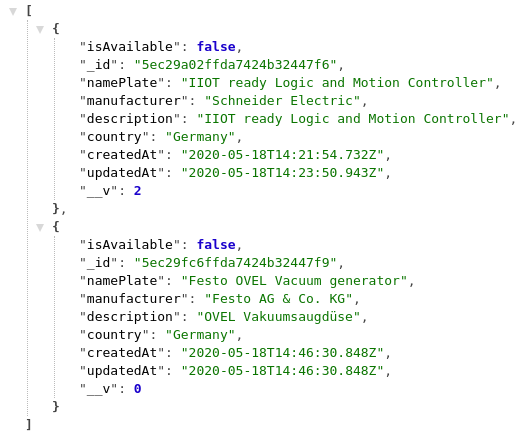
\includegraphics[width=0.8\textwidth]{json}
		\fonte{O autor.}
	\end{figure}

	
\section{ API de interação Cliente-Servidor }

	Para fins de escrita e pelo Cliente a fins de leitura é realizado por meio de uma API REST.
	
	A API REST é invocada como uma interface para acesso aos serviços de um AAS Servidor, podendo extrair dados internos de sua MDP e executar operações CRUD (criação, leitura, atualização e exclusão).
	
\chapter{Publicações decorrentes do trabalho}
\label{cha:publicacoes}

	\textbf{Publicação 1} \cite{vitoi2019logistica}
	\begin{itemize}
		\item VITOI, H. A.; JUNQUEIRA, F.; MIYAGI, P. E. Análise de implementação de IoT na cadeia logística. In: ABEPRO. 39\textsuperscript{o} Encontro Nacional de Engenharia de Produção. [S.l.], 2019.
	\end{itemize}
	
	\bigskip

	\textbf{Publicação 2} \cite{coda2019bigdata}
	\begin{itemize}
		\item CODA, F. A.; SALLES, R. M.; VITOI, H. A; PESSOA, M. A. O.; MOSCATO, L. A.; FILHO, D. S.; JUNQUEIRA, F.; MIYAGI, P. E. Big data on machine to machine integrations requirement analysis within industry 4.0. In: SPRINGER. Doctoral Conference on Computing, Electrical and Industrial Systems (DoCEIS) - Technological Innovation for Industry and Service Systems. [S.l.], 2019. p. 247–254. 
	\end{itemize}

\chapter{Cronograma de atividades}
\label{cha:cronograma}

	O cronograma cumpridos nos anos de 2018 e 2019 é mostrado na \autoref{tab:cronograma-18-19}.
	
	\begin{table}[htb]
		\centering
		\caption{Cronograma detalhado de atividades em 2018 e 2019.}
		\label{tab:cronograma-18-19}
		\makebox[\textwidth][c]{\footnotesize
		\begin{tabular}{|c|c|c|c|c|c|c|c|c|c|c|c|c|}
			\hline
			%
			& \multicolumn{2}{c|}{\textbf{2018}}
			& \multicolumn{6}{c|}{\textbf{2019}} \\
			
			\hline
			Etapas
			& \begin{tabular}[c]{@{}c@{}}set/\\out\end{tabular} 
			& \begin{tabular}[c]{@{}c@{}}nov/\\dez\end{tabular} 
			& \begin{tabular}[c]{@{}c@{}}jan/\\fev\end{tabular} 
			& \begin{tabular}[c]{@{}c@{}}mar/\\abr\end{tabular} 
			& \begin{tabular}[c]{@{}c@{}}mai/\\jun\end{tabular} 
			& \begin{tabular}[c]{@{}c@{}}jul/\\ago\end{tabular} 
			& \begin{tabular}[c]{@{}c@{}}set/\\out\end{tabular} 
			& \begin{tabular}[c]{@{}c@{}}nov/\\dez\end{tabular} \\ 
			
			\hline
			Cumprimento dos créditos 
			& \cellcolor[HTML]{9AFF99}C
			& \cellcolor[HTML]{9AFF99}C 
			& \cellcolor[HTML]{9AFF99}C 
			& \cellcolor[HTML]{9AFF99}C 
			& \cellcolor[HTML]{9AFF99}C 
			& \cellcolor[HTML]{9AFF99}C 
			&
			& \\
			
			\hline
			Levantamento bibliográfico
			& \cellcolor[HTML]{9AFF99}C
			& \cellcolor[HTML]{9AFF99}C
			& \cellcolor[HTML]{9AFF99}C
			& \cellcolor[HTML]{9AFF99}C
			& \cellcolor[HTML]{9AFF99}C
			& \cellcolor[HTML]{9AFF99}C
			& \cellcolor[HTML]{9AFF99}C
			& \cellcolor[HTML]{9AFF99}C \\
			
			\hline
			Desenvolvimento do projeto
			&
			&
			& \cellcolor[HTML]{9AFF99}C
			& \cellcolor[HTML]{9AFF99}C
			& \cellcolor[HTML]{9AFF99}C
			& \cellcolor[HTML]{9AFF99}C
			& \cellcolor[HTML]{9AFF99}C
			& \cellcolor[HTML]{9AFF99}C \\ 
			
			\hline
			Exame de Qualificação
			&
			&
			&
			&
			&
			&
			&
			& \\
			
			\hline
			Defesa da dissertação
			&
			&
			&
			&
			&
			&
			&
			& \\
			\hline
			
		\end{tabular}}
		\fonte{O autor.}
	\end{table}

	O cronograma planejada no ano de 2020 é mostrado na \autoref{tab:cronograma-20}

	\begin{table}[htb]
		\centering
		\caption{Cronograma detalhado planejado para 2020.}
		\label{tab:cronograma-20}
		\makebox[\textwidth][c]{\footnotesize
			\begin{tabular}{|c|c|c|c|c|c|c|c|c|c|c|c|c|}
				\hline
				%
				& \multicolumn{6}{c|}{2020} \\
				
				\hline
				Etapas
				& \begin{tabular}[c]{@{}c@{}}jan/\\fev\end{tabular}
				& \begin{tabular}[c]{@{}c@{}}mar/\\abr\end{tabular}
				& \begin{tabular}[c]{@{}c@{}}mai/\\jun\end{tabular}
				& \begin{tabular}[c]{@{}c@{}}jul/\\ago\end{tabular}
				& \begin{tabular}[c]{@{}c@{}}set/\\out\end{tabular}
				& \begin{tabular}[c]{@{}c@{}}nov/\\dez\end{tabular} \\
				
				\hline
				Cumprimento dos créditos
				&
				&
				&
				&
				&
				& \\
				
				\hline
				Levantamento bibliográfico
				& \cellcolor[HTML]{9AFF99}C
				& \cellcolor[HTML]{9AFF99}C
				& \cellcolor[HTML]{9AFF99}C
				& \cellcolor[HTML]{9AFF99}C
				& \cellcolor[HTML]{FFCB2F}A
				& \cellcolor[HTML]{FFCB2F}A \\
				
				\hline
				Desenvolvimento do projeto
				& \cellcolor[HTML]{9AFF99}C
				& \cellcolor[HTML]{9AFF99}C
				& \cellcolor[HTML]{9AFF99}C
				& \cellcolor[HTML]{9AFF99}C
				& \cellcolor[HTML]{FFCB2F}A
				& \\
				
				\hline
				Exame de Qualificação
				&
				& 
				&
				&
				& \cellcolor[HTML]{FFCB2F}A
				& \\
				
				\hline
				Defesa da dissertação
				&
				&
				&
				&
				&
				& \cellcolor[HTML]{FFCB2F}A \\
				\hline
				
		\end{tabular}}
		\fonte{O autor.}
	\end{table}

	A data estipulada para defesa da dissertação pode ser postergada conforme a necessidade de refinamento do projeto, adicionando-se mais meses para levantamento bibliográfico e desenvolvimento do projeto, respeitando-se o prazo máximo para depósito da dissertação. 
	
	Disciplinas cursadas nos períodos 2018/3, 2019/1 e 2019/2:
	\begin{itemize}
		\item PMR5024 - Simulação de Sistemas;
		\item PTC5751 - Internet das coisas;
		\item PEA5003 - Sistemas Inteligentes de Transporte;
		\item PMR5023 - Modelagem e Análise de Sistemas;
		\item PTR5744 - Pesquisa Operacional;
		\item PRO5807 - Logística e Cadeia de Suprimentos;
		\item PMR5402 - Controle de Sistemas.
	\end{itemize}

	% Dizer no que as disciplinas ajudaram no trabalho. 
	

\chapter{Considerações finais}
\label{cha:conclusao}

	A elaboração de uma arquitetura comum para o compartilhamento de informações do ativo é essencial para que haja consistência e interoperabilidade entre os membros da cadeia de suprimentos adotando este sistema.
	
	Este trabalho traça um modelo de compartilhamento de informações por meio de \textit{Web Services} utilizando como arquitetura de base o RAMI4.0, que é atualmente o principal modelo de arquitetura de referência para a Indústria 4.0. 
	
	O mapeamento das operações de um \textit{Web Service} para o eixo ``Camadas'' do RAMI4.0 por meio de diagramas PFS permite a visualização dos fluxos de atividades ocorridas durante todo o processo de consumo da memória digital do produto, assim como estabelece as responsabilidades de cada camada para todo o processo. 
	
	Foi abordado também como a MDP pode contribuir na melhoria de projeto do produto e na eficiência operacional da dinâmica da cadeia de suprimentos e como isso propicia o surgimento de novos modelos de negócio baseado em dados (\textit{data-driven}).
	
	Uma visão da MDP sobre o eixo ``Ciclo de Vida e Cadeia de Valor'' do RAMI4.0 é abordada, discutindo melhor o porquê e as atribuições dos AASs como ``tipos'' e como ``instâncias''.
	
	Por fim, são propostas possíveis informações relevantes à cadeia de suprimentos a serem salvas na MDP indicando quando esta informação devem ser armazenadas, onde e a qual cliente esta informação seria de interesse.

% Elementos pós-textuais
\postextual
\bibliography{bibliografia}

\end{document}
